 \documentclass{article}
\usepackage{graphicx} 
\usepackage[dutch]{babel}
\usepackage{geometry}
\usepackage{subcaption}
\usepackage{ragged2e}
\usepackage{xcolor}
\usepackage{tabularray}
\UseTblrLibrary{varwidth}  % <===
\usepackage{enumitem}
\usepackage{etoolbox}
\AtBeginEnvironment{longtblr}%
{
	\setlist[itemize]{nosep,
		label=--, % or \textbullet
		wide,
		after=\end{minipage},
	before=\begin{minipage}[t]{\linewidth}\RaggedRight
	}
}
\newcommand{\lto}{\mathbin{\to}}

\begin{document}
	\sffamily
	\begin{titlepage}
		\centering
		\vfill
		{\bfseries\Huge
			Verslag Tinlab Advanced Algorithms \\
			\vskip2cm
		}
		{\bfseries\Large
			Galvin Bartes 0799967\\
		}
		{
			\bfseries\normalsize
			176-671\\
			\vskip1cm
			\today\\
		}    
		\vfill
		
\includegraphics[width=4cm]{logohr.png} % also works with logo.pdf
		\vfill
		\vfill
	\end{titlepage}
	\newpage
	\tableofcontents
	
	\newpage
	\section{Inleiding}
	
	
	\paragraph{Algemeen}
	
	Het ministerie van verkeer en Waterstaat wil in het kader van het klimaatakkoord en onderzoek laten uitvoeren naar de staat van het sluizenpark in Nederland. Het onderzoek moet zich richten op het ontwerpen en ontwikkelen van een geautomatiseerd sluismodel dat geschikt is voor een brede toepassing. In het onderzoek moet naar voren komen wat de huidige staat is van de sluizen met oog op veiligheid, efficiëntie, capaciteit, onderhoud, duurzaamheid en automatisering. Het onderzoek geeft aan hoe een volledig model worden opgeleverd opdat ontwerp van verschillend volledig geautomatiseerde sluizen in de toekomst geautomatiseerd kunnen worden.  
	
	
	
	
	%%%%%%%%%%%%%%%%%%%%%%%%%%%%%%%%%%%%%%%%%%%%%%%%%%%%%%%%%%%%%%%%%
	
	\paragraph{Probleemanalyse}
	
	Na grondige analyse van het Nederlandse sluizenpark is gebleken dat renovatie van een groot aantal sluizen noodzakelijk is.  Uit een eerste verkenning is gebleken  dat het gecombineerd renoveren en automatiseren van het Nederlandsesluizenpark een aanzienlijke verbetering kan opleveren t.a.v. 
	Op  het  ministerie  van  infrastructuur  enwaterstaat is helaas onvoldoende kennis van ict en systemen aanwezig om eenen ander uit te voeren 
	
	\paragraph{Waarom nu}
	In  het  kader  van  het  onlangs  afgesloten  klimaatakkoord  heeft  de  Nederlandseoverheid  daarom  besloten  over  te  gaan  tot  een  ingrijpende  renovatie  van  dediverse  sluizen  die  ons  land  rijk  is.     
	
	\paragraph{Gewenst resultaat }
	
	
	Wij vragen u een model (of een onderling samenhangend aantal modellen)aan  te  leveren,  opdat  ontwerpen  van  verschillende,  volledig  geautomatiseerdesluizen in de toekomst gerealiseerd kunnen worden. 
	Zoals  gesteld  in  de  brief  is  het  de  bedoeling  dat  een  sluis  gemodelleerd  wordten  dat  bewezen  kan  worden  dat  de  te  bouwen  sluis  een  aantal  eigenschappenbezit.  
	
	Ons doel is een uppaal model van een sluis op te leveren. We wilen een fysiek systeem vastleggen in software, ofwel een domeini uit de echte wereld overplaatsen naar het conditionele. De phenomenen  uit de echte wereld wprden gemonitored met sensoren.
	De phenomenen uit de wereld worden kenbaar gemaakt aan het softwaresystem in de vorm van variabele data.
	Welke data wordt opgevangen, opgeslagen en uitgelezen wrdt vastgelegd in de requirements. De manier waarop dit gebeurt wordt vastegelegd in specificaties.
	De requirements worden verkregen door requirements engineers. Dit variert  van concepten en best-practices uit observaties, interviews, stakehoders anaysis, focus group, document analysis, het verkennen van user requirements, 
	task analysis, surveys en problem analysis.
	Requirements worden onderverdeeld in functioneel en niet-functioneel.
	Functionele requirements omschrijven de klantwens, ofwel functie en gedrag. Niet-functionele requirements/eisen zijn beperkt  tot vereisten die aan systemen worden opgelegd. Ze hebben betrekking op kwaliteitsattributen als: schaalbaarheid, onderhoudbaarheid, beveiliging, betrouwbaarheid.
	Belangrijk is de vraag wat is een goed model. Voor het testen van een goed model of een specificatie zij verschillendetechnieken. In de biomedische wereld wordt er een onderscheidt gemaakt tussen  in vivo "levendig" in vitro "afgeschieden experiment" en insilico "een gecomputeriseerd model".
	
	\paragraph{Scope}
	
	He gaat om het simuleren van een geautomatiseerde sluis. Wat voor type sluis wordt niet gemeld en ook niet uit welke onderdelen. Belangrijk is dat het model werkt en dat het voldoet aan de eisen die gebaseerd zijn op basis van literatuuronderzoek, observatie, interviews, brainstorming of een andere vorm van requirements elicitation.
	
	\paragraph{Onderzoeksvragen }
	
	Hoe kan een geautomatiseerde sluis worden gemodeleerd met oog op ontwikkel- en onderhoudskosten,veiligheid, efficientie en capaciteit
	
	
	
	
	
	\begin{enumerate}
		
		\item Welke requirements en kwaliteitseisen komen naar voren bij de analyse van een rampenonderzoek
		\item Welke veiligheidseisen er zijn voor sluizen in nederland. 
		\item Hoe kan in uppaal  een model worden getest dat voldoet aan de requirements/eisen volgens het rampenonderzoek?
	\end{enumerate}
	
	%%%%%%%%%%%%%%%%%%%%%%%%%%%%%%%%%%%%%%%%%%%%%%%%%%%%%%%%%%%%%%%%%
	
	
	\paragraph{Design goals}
	Het systeem moet minimaal aan de volgende prestatie eisen voldoen 
	
	\begin{enumerate}
		\item   Requirements gebaseerd op rampenanalyse
		\item Model testbaar in upaal
	\end{enumerate}
	
	
	
	%%%%%%%%%%%%%%%%%%%%%%%%%%%%%%%%%%%%%%%%%%%%%%%%%%%%%%%%%%%%%%%%%
	\paragraph{Leeswijzer}
	In  de methodologie wordt de lezer uitgelegd met welke methoden de onderzoeksvragen zijn beantwoord. In het hoofdstuk Onderzoek worden alle resultaten behandeld die naar voren zijn gekomen bij het deskresearch. De analyse van de verzamelde data wordt gedaan in het hoofdstuk analyse. Hierin wordt behandeld zoekopdracht naar IoT cloud platforms, feature extractie, prijs-berekening en prijs-feature vergelijking. In het ontwerp komen de uml diagrammen en systeemschetsen naar voren. In de  de hoofdstukken Prototype, IoT cloud en Firmware wordt de implementatie behandeld van het IoT cloud platform in een bestaand project.
	
	%%%%%%%%%%%%%%%%%%%%%%%%%%%%%%%%%%%%%%%%%%%%%%%%%%%%%%%%%%%%%%%%%
	
	\newpage
	
	
	
	
	
	\section{Theoretisch kader}
	In het eerste hoofdstuk is duidelijk geworden wat de onderzoeksvraag is, namelijk ‘Hoe kan een geautomatiseerde sluis worden gemodeleerd met oog op ontwikkel- en onderhoudskosten,veiligheid, efficientie en capaciteit’. Door de toenemende complexiteit van systemen is het gebruik van modellen en de toepassing van timebased model checking  op industriele controle systemen een manier van modelleren van het systeem en de requirements zodat er een bijdagre kan worden geleverd aan de acceptatie van  simulatie-/modeltechniek voor de industrie.\cite{RijnensupervisorsynthesisLock}. Of dit ook het geval is bij het modellereren van sluizen is nu de vraag.
	
	De bestudering van rampen aan de hand van het vier-variabelen model biedt maakt het analyseren mogelijk van rampsituaties. Van een aantal rampen is een beschrijving gegeven met datum, plaats en oorzaak. De analyse van de 4-variabelen modellen zal gebruikt worden voor de requirementsdefinitie, ontwerp en ontwikkeling van het sluismodel. 
	
	De verschillende factoren en achtergronden die  samenhangen met het modelleren van een sluis zullen in dit hoofdstuk toegelicht worden. Bovendien worden er hypotheses gevormd die de basis vormen voor debeantwoording van de onderzoeksvraag. 
	
	\subsection{Begrippen, tools en literatuur}
	
	\paragraph{Wat is uppaal}
	Uppaal is een geïntegreerde toolomgeving voor het modelleren, simuleren en verifiëren van real-time systemen, gezamenlijk ontwikkeld door Basic Research in Computer Science aan de Universiteit van Aalborg in Denemarken en de afdeling Informatietechnologie aan de Universiteit van Uppsala in Zweden. Het is geschikt voor systemen die kunnen worden gemodelleerd als een verzameling niet-deterministische processen met een eindige controlestructuur en klokken met reële waarde, die communiceren via kanalen of gedeelde variabelen . Typische toepassingsgebieden zijn met name real-time controllers en communicatieprotocollen, waarbij timingaspecten van cruciaal belang zijn. %\cite{uppaalFeatures}
	
	\paragraph{Wat is statistical model checking?}
	Dit verwijst naar verschillende technieken dfie worden gebruikt voor de monitoring van een systeem. Daarbij wordt vooral gelet op een specifieke eigenschap. Met de resultaten van de statsitieken wordt de juistheid van een ontwerp beoordeeld. Statistisch model checking wordt onder andere toegepast in systeembiologie, software engineering en industriele toepassingen.
	%\cite{verimagStatsModelChecking}.
	\cite{inriaStatsMoodCheck}
	\cite{ buddeModelChecker}
	%\cite{AGHASuervey }
	
	\paragraph{Waarom gebruiken we statistisch model checking?}
	Om de bovenstaande problemen te overwinnen stellen we voor om te werken met Statistical Model Checking , een aanpak die onlangs is voorgesteld als alternatief om een uitputtende verkenning van de toestandsruimte van het model te vermijden. Het kernidee van de aanpak is om een aantal simulaties van het systeem uit te voeren, deze te monitoren en vervolgens de resultaten uit het statistische gebied te gebruiken (inclusief het testen van sequentiële hypothesen of Monte Carlo-simulaties) om te beslissen of het systeem aan de eigenschap voldoet of niet. mate van vertrouwen. Van nature is SMC een compromis tussen testen en klassieke modelcontroletechnieken. Het is bekend dat op simulatie gebaseerde methoden veel minder geheugen- en tijdintensief zijn dan uitputtende methoden, en vaak de enige optie zijn.
	\cite{inriaStatsMoodCheck}Alternatieve tools voor Uppaal zijn Asynchronous Events,Vesta en MRMC.
	
	
	\paragraph{MODE CONFUSION }
	Mode confusion treed op als geobserveerd gedrag van een technisch systeem niet past in het gedragspatroon dat de gebruiker in zijn beeldvorming heeft  en ook niet met voorstellingsvermogen kan bevatten.
	
	\paragraph{Wat is automatiseringsparadox}
	Gemak dient de mens. Als er veel energie wordt gestoken in de ontwikkeling van hulmiddelen die taken van werknemers overemen heeft dat tot resultaat dat veel productieprocessen worden geautomatiseerd. De vraag is dan of vanuit mechnisch wereldpunt de robot niet de rol van de mens overneemt en of de mens nog de kwaliteiten heeft om het werk zelf te doen.
	\cite{bicker21102016automatiseringsparadox}
	\cite{vseautoparadox}
	\cite{blogxot21112016slimapparaat}
	
	
	
	\paragraph{4 variabelen model}
	
	Er zijn veel veiligheidskritische computersystemen nodig voor het bewaken en besturen van fysieke processen
	processen. Het viervariabelenmodel, dat al bijna met succes in de industrie wordt gebruikt
	veertig jaar, helpt het gedrag van en de grenzen tussen het fysieke te verduidelijken
	processen, invoer-/uitvoerapparaten en software. \cite{ImplementabilityOf4VarSCP2015}
	
	
	
	Het 4 variabelen model kort toegelicht
	Monitored variabelen: door sensoren gekwantificeerde fenomenen uit de omgeving, bijv temperatuur
	
	Controlled variabelen: door actuatoren bestuurde fenomenen uit de omgeving
	Gecontroleerde variabelen kunnen bijvoorbeeld de druk en de temperatuur zijn
	in een kernreactor, terwijl gecontroleerde variabelen ook visuele en hoorbare alarmen kunnen zijn
	als het uitschakelsignaal dat een reactorsluiting initieert; wanneer de temperatuur of druk bereikt
	abnormale waarden, de alarmen gaan af en de uitschakelprocedure wordt gestart
	
	Input variabelen: data die de software als input gebruikt
	Hier modelleert IN de ingangshardware-interface (sensoren en analoog-naar-digitaal-omzetters) en
	relateert waarden van bewaakte variabelen aan waarden van invoervariabelen in de software. De invoervariabelen modelleren de informatie over de omgeving die beschikbaar is voor de software. Bijvoorbeeld,
	IN zou een druksensor kunnen modelleren die temperatuurwaarden omzet in analoge spanningen; Deze spanningen worden vervolgens via een A/D-omzetter omgezet in gehele waarden die zijn opgeslagen in een register dat toegankelijk is voor de computer
	software.
	
	Output variabelen: data die de software levert als output
	De uitgangshardware-interface (digitaal-naar-analoog converters en actuatoren) is gemodelleerd
	door OUT, dat waarden van de uitvoervariabelen van de software relateert aan waarden van gecontroleerde variabelen. Een uitvoervariabele kan bijvoorbeeld een Booleaanse variabele zijn die door de software is ingesteld met de
	begrijpen dat de waarde true aangeeft dat een reactorsluiting zou moeten plaatsvinden en de waarde
	false geeft het tegenovergestelde aan
	
	
	\paragraph{6 Variable model}
	Een uitbreiding van een 4-variabelen model is het 6-variabelen model.
	Optitatieve statements omschrijven de omgeving zoals we het willen zien vanwege de machine. 
	Indicatieve statements omschrijven de omgeving zoals deze is los van de machine. 
	Een requirement is een optitatief statement omdat ten doel heeft om de klantwens uit te drukken in een softwareontwikkel project. 
	Domein kennis bestaut uit indicatieve uitspraken die vanuit het oogpunt van software ontwikkeling relevant zijn. 
	Een specificatie is een optitatief statement met als doel direct implementeerbaar te zijn en ter verondersteuning van het nastreven en realiseren van de requirements. 
	Drie verschillende type domeinkennis: domein eigenschappen, domein hypothesen, en verwachtingen. 
	Domein eingenschappen  zijn beschrijvende statementsover een omgeving en zijn feiten. Domein hypotheses  zijn ook beschrijvende uitspraken over een omgeving, maar zijn aannames. 
	Verwachtingen zijn ook aannames, maar dat zijn voorschrijvende uitspraken die behaald worden door actoren als personen, sensoren en actuators. 
	
	%	\paragraph{World and machine samenvatting}
	%	Inderdeel van deze cursus is de studie van het artikel World as a machine \cite{jacksonworldmachine}
	%	Software engineering maakt het gebruik van fysieke apparaten mogelijk. Het is een beschrijving van de machine. Het doel van een machine ligt in de wereld.
	%	Commando afhandeling wordt niet  beoordeeld door examinering van de software, maar door te kijken naar de kwaliteit van de geprogrammeerde documenten en het gebruik, gemak en voldoening voor de operators.
	%	Het probleem is de requirement dat ligt in de wereld en de machine is de oplossing die we bedenken. De  relatie tussen machine en wereld  blijkt uit de volgende 4 facetten:
	%	\begin{itemize}
		%		\item 1 modelling facet:
		%		\item interface facet:
		%		\item engineering facet:
		%		\item problem facet: requirements, specificaties en programmas zijn subsets van  domeinen bestaande uit wereldlijke en machinale fenomenen. Decompositie van  probleem verloopt parralel en niet hierarchisch.
		%	\end{itemize}
	%	denial bij knowledge: net meer het wiel uitvinden
	%	denial by hacking: obsessief toegewijs aan interactie met computers
	%	denial by abstraction: aoftwareproblemen kunnen bevangen worden in enkele simpele woorden. Het moeilijke is problemen op te splitsen.
	%	Denial by vageueness: vaag taalgebruik om probleem te verhullen
	%	
	%	Formal recognizable description
	%	Gebruikte event als grondterm en geen english noun. Dit is reognizable.
	%	De wereld is niet strongly typed
	%	verschil tussen aannemen(optatief) en willen zien(indicatief)
	%	
	%	
	%	
	%	
	%	\paragraph{Systeem vs software requirement}
	%	Ter verduidelijking van het het verschil tussen systeemrequirement en softwarerequirement hieronder een overzicht:
	%	
	%	
	%	Een system requirement is een uitspraak over wereld fenomenen (gedeeld of niet) of doelen
	%	die bereikt moeten worden. En systeem requirement is met enige regelmaat informeel, niet precies geformuleerd.
	%	Systemen gaan een zekere interactie aan met hun omgeving:Sensoren: meten fenomenen uit de omgeving (temperatuur,druk, licht, geluid, etc.). Actuatoren: veranderen iets in de omgeving (mechanische,electrisch, pneumatisch, etc.)
	%	
	%	Een software requirement/specifcatie is een uitspraak over gedeelde fenomenen of doelen die de machine
	%	moet bereiken middels de onderdelen waar die machine uit of middels de fenomenen waar de machine controle
	%	over heeft. Is doorgaans preciezer, meetbaar, exact geformuleerd.
	%	
	%	Software kan niet direct communiceren met de buitenwereld.Snapt derhalve niets van de buitenwereld. Kan alleen maar bestaan in en communiceren met het systeem.
	%	
	%	
	%	\paragraph{Requirementsengineering}
	%	
	%	Om de juiste requirements te verzamelen en selecteren hebben we meer kennis nodig van de methoden hiervoor gebruikt in het domein van requirementsengineering.
	%	\cite{jonkerTreurKlush200informativeAgents}
	%	\cite{boehmBoseLeeRequirementsNegotiations}
	%	\cite{muHungJinLiu2013inconsistencyReqs}
	%	\cite{hunterNuseibeh1996manageSpecs}
	%	
	%	\cite{zavePamela4darkCorners}
	%	\cite{zavePAmela1997regEngineering}.
	%	
	%	%%%%%%%%%%%%%%%%%%%%%%%%%%%%%%%%%%%%%%%%%%%%%%%%%%%%%%%%%%%%%%%%%
	%	
	%	what is a good software specification
	%	
	%	
	%	\begin{itemize}
		%		\item Een goed model heeft een duidelijk gespecificeerd modelleringsobject, dat wil zeggen dat het duidelijk is wat het model beschrijft.  %A good model has a clearly specified object of modelling, that is, it is clear what thing the model describes. 
		%		\item Een goed model heeft een duidelijk omschreven doel en draagt (idealiter) bij aan de realisatie van dat doel. %A good model has a clearly specified purpose and (ideally) contributes to the realization of that purpose.
		%		\item Een goed model is traceerbaar: elk structureel element van een model (1) komt overeen met een aspect van het modelobject, of (2) codeert voor impliciete domeinkennis, of (3) codeert voor een aanvullende aanname. %A good model is traceable: each structural element of a model either (1) corresponds to an aspect of the object of modelling, or (2) encodes some implicit domain knowledge, or (3) encodes some additional assumption. 
		%		\item Een goed model is waarheidsgetrouw: relevante eigenschappen van het model moeten ook worden overgedragen op (behouden voor) het object van modellering. %A good model is truthful: relevant properties of the model should also carry over to (hold for) the object of modelling.
		%		\item Een goed model is eenvoudig (maar niet te eenvoudig). %A good model is simple (but not too simple).
		%		\item Een goed model is uitbreidbaar en herbruikbaar, dat wil zeggen dat het is ontworpen om te evolueren en te worden gebruikt buiten het oorspronkelijke doel. %A good model is extensible and reusable, that is, it has been designed to evolve and be used beyond its original purpose. 
		%		\item Er is een goed model ontworpen en gecodeerd voor interoperabiliteit en het delen van semantiek. %A good model has been designed and encoded for interoperability and sharing of semantics. 
		%	\end{itemize}
	%	
	%	
	%	\cite{fvaandrager2322010Goodmodel}. Meer artikelen zijn: 
	%	\cite{onix01102022devopmodel}
	%	\cite{sulemani04012021softwareprocesmodel}
	%	\cite{globalluxsoft18102017softdev}
	%	\cite{wiegers30052022SRS}
	%	\cite{muller06092020goodspecification}
	%	\cite{informit30062008reqmanagement}
	%	\cite{altexsoft15092020writingSRS}
	%	
	%	
	%	\paragraph{Wat is een sluis}
	%	Een sluis is ook een scheiding tussen 2 wateren, maar met deuren. Hierdoor is het mogelijk het waterpeil te beïnvloeden. Sluizen reguleren het waterpeil zodat schepen kunnen passeren. Een stuw is een vaste of beweegbare afdamming tussen 2 wateren. \cite{rijkSluisdef}
	%	
	%	\cite{woudagemaalSluizen}
	%	\cite{bardetsluizenAmsterdam}
	%	\cite{historischesluizen}
	%	Een model van een sluispasssage kan worden gemodelleerd met procestates zoals het model aangeboden door Rijkswaterstaat
	%	\begin{center}
		%		
		%		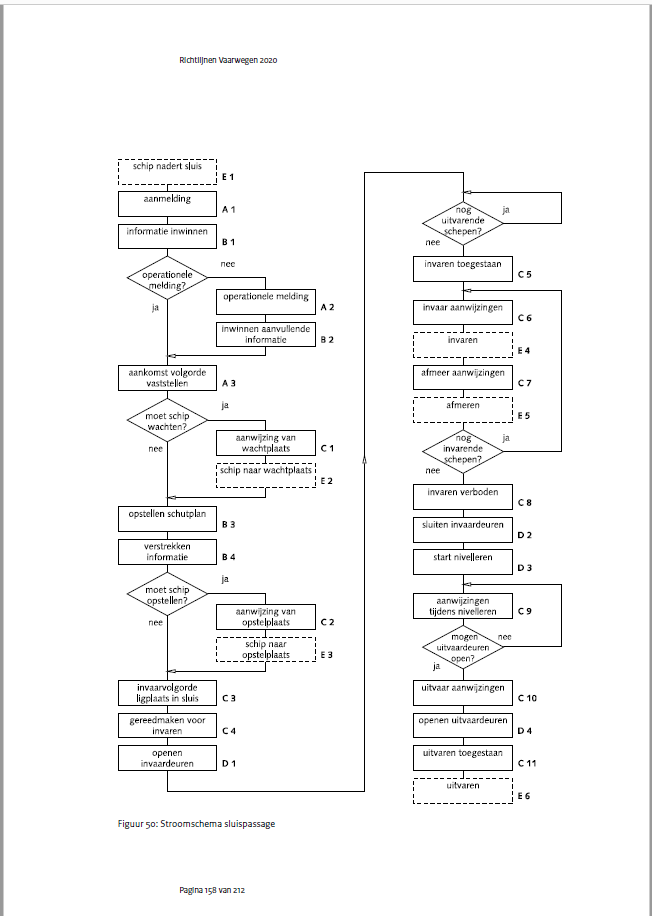
\includegraphics[width=10cm]{stroomschema_sluispassage.png} % also works with logo.pdf
		%		
		%	\end{center}
	%	
	%	
	%	
	%	
	%	\cite[p.79~--113]{rijksoverheidSluizen}
	%	\cite[p.159]{rijksoverheidSluisStroomschema},
	%	
	%	
	%	
	%	
	%	\paragraph{Recente ontwikkelingen op het gebied van sluisautomatisering}
	%	
	%	Het ministerie van verkeer en Waterstaat wil in het kader van het klimaatakkoord en onderzoek laten uitvoeren naar de staat van het sluizenpark in Nederland. Het onderzoek moet zich richten op het ontwerpen en ontwikkelen van een geautomatiseerd sluismodel dat geschikt is voor een brede toepassing. In het onderzoek moet naar voren komen wat de huidige staat is van de sluizen met oog op veiligheid, efficiëntie, capaciteit, onderhoud, duurzaamheid en automatisering. Het onderzoek geeft aan hoe een volledig model worden opgeleverd opdat ontwerp van verschillend volledig geautomatiseerde sluizen in de toekomst geautomatiseerd kunnen worden.  
	
	
	\subsection{Rampen}
	
	\newline \indent Voor deze studie is onderzoek gedaan naar verschillende rampen aan de hand van het vier variabelen model.
	Elke ramp op deze manier categoriseren  kan ons helpen te bepalen in hoeverre requirements een rol kunnen spelen in de veiligheid van ons model.
	
	
	% 
	% 
	%\paragraph{ethiek}
	%
	%
	%Ethiek 
	%
	%
	%
	%persuasive technology 
	%https://www.humanetech.com/youth/persuasive-technology 
	%\cite{humanTechpersuasiveTech}
	%https://www.minddistrict.com/blog/persuasive-technology-new-insights-in-behavioural-change 
	%https://www.sciencedirect.com/book/9781558606432/persuasive-technology 
	%https://spectrum.ieee.org/how-persuasive-technology-can-change-your-habits 
	%\cite{rezenfeld01012018persuasiveTecgHabits}
	%https://www.frontiersin.org/articles/10.3389/frai.2020.00007/full 
	%\cite{aldenaini28042020persuasiveTechTrends}
	%https://psmag.com/environment/captology-fogg-invisible-manipulative-power-persuasive-technology-81301 
	%\cite{larson14062017persuasivetechmanipulates}
	%https://www.makeuseof.com/what-is-persuasive-technology/ 
	%\cite{tanzem22012022persuasivetechchanginglives}
	%https://lib.ugent.be/catalog/rug01:001235489 
	%https://cyberpsychology.eu/article/view/12270 
	%\cite{tikkakuddonenpersuasiveTechnology}
	%
	
	%
	%
	%\paragraph{Ondeerzoeksresultaten naar sluisbeveiliging}
	%
	%
	%
	%Verouderde computersystemen zijn door de jaren heen gekoppeld aan netwerken, zodat ze op afstand te besturen zijn. Dit zorgt ervoor dat systemen kwetsbaar zijn voor aanvallen van buitenaf. De beveiliging is in de loop der jaren niet voldoende ontwikkeld om de infrastructuur goed te beveiligen.
	%
	%Volgens het onderzoek is er de afgelopen jaren wel het nodige geïnvesteerd om de beveiliging op te schroeven, maar deze maatregelen zijn nog onvoldoende doorgevoerd.
	%https://www.nu.nl/internet/5814282/rekenkamer-waterwerken-niet-goed-beveiligd-tegen-cyberaanvallen.html
	%\cite{hdsr30092022lichtprojectieswaterliniesluizen}
	%rapport Digitale dijkverzwaring: cybersecurity en vitale waterwerken 
	%Crisisdocumentatie is verouderd en er worden geen volwaardige pentesten uitgevoerd. Uit het onderzoek blijkt dat nog niet alle vitale waterwerken rechtstreeks zijn aangesloten op het Security Operations Center (SOC) van Rijkswaterstaat. Hierdoor bestaat het risico dat RWS een cyberaanval niet of te laat detecteert. De minister van Infrastructuur en Waterstaat moet nog stappen zetten om aan de eigen doelstellingen voor cybersecurity te voldoen
	%De Algemene Rekenkamer beveelt de minister van Infrastructuur en Waterstaat ook aan om het actuele dreigingsniveau te onderzoeken en te besluiten of extra mensen en middelen nodig zijn. Ook is het voor een snelle en adequate reactie op een crisissituatie van essentieel belang dat informatie up-to-date is. Pentesten zouden integraal onderdeel uit moeten maken van de cybersecuritymaatregelen bij vitale waterwerken. Verder zou moeten worden bezien of medewerkers van het SOC beter moeten worden gescreend.
	%
	% 
	%
	%
	%\cite{thkwaterwerken}
	%Het crisismodel kan beter, is de derde deelconclusie van de Algemene Rekenkamer. Er is geen specifiek scenario voor een crisis die wordt veroorzaakt door een cyberaanval. Ook ontbreekt inzicht in de effecten van een cybercrisis op andere sectoren, de zogeheten cascade-effecten. Tevens is de crisisdocumentatie op onderdelen verouderd.
	%
	%\cite{rekenkamercybersecWater}
	%Ook maakt cyberveiligheid nog geen volwaardig onderdeel uit van reguliere inspecties.’ De Rekenkamer hamert erop dat alle vitale waterinfrastructuur zo snel mogelijk op het SOC wordt aangesloten. Ook zouden werknemers van Rijkswaterstaat die belangrijke waterkeringen bedienen beter gescreend moeten worden op hun antecedenten. Sollicitanten hoeven nu slechts een Verklaring Omtrent Gedrag te overleggen, maar dat is een heel lichte toets.
	%
	%\cite{hackerWaterwerk}
	%deltawerken
	%
	%\cite{kramerZeeland}
	%Volgens Rijkswaterstaat is het kostbaar en technisch uitdagend om klassieke automatiseringssystemen te moderniseren en wordt er daarom vooral ingezet op detectie van aanvallen en een adequate reactie daarop.
	%Uit het onderzoek blijkt dat Rijkswaterstaat de afgelopen jaren zelf van alle tunnels, bruggen, sluizen et cetera heeft vastgesteld welke cyberveiligheidsmaatregelen moeten worden genomen. Een groot deel van die maatregelen (ongeveer 60\%) was begin 2018 ook al uitgevoerd, maar Rijkswaterstaat ziet onvoldoende toe op de uitvoering van het resterend deel en heeft geen actueel overzicht van de overgebleven maatregelen.
	%De minister heeft een aantal waterwerken die Rijkswaterstaat beheert als vitaal aangewezen. . Uit het onderzoek blijkt dat nog niet alle vitale waterwerken rechtstreeks zijn aangesloten op het Security Operations Center (SOC) van Rijkswaterstaat. De ambitie om eind 2017 bij alle vitale waterwerken cyberaanvallen direct te kunnen detecteren was in het najaar van 2018 daarmee nog niet gerealiseerd. Hierdoor bestaat het risico dat RWS een cyberaanval niet of te laat detecteert.
	%
	%\cite{cybersecWaterwerk}
	%Over de cyberbeveiliging van gemeenten en waterschappen wordt al langer geklaagd. Zo meldde EenVandaag al in 2012 dat rioolgemalen en sluizen gemakkelijk van afstand te bedienen waren, onder meer door bijzonder slechte wachtwoorden.
	%
	%\cite{cybersecWaterschappen}
	%Rittal doet onderzoek naarop afstand besdienbare sluizen
	%
	%\cite{cybersecZuidHolland}
	%Beveiligde VPN
	%M2M Services levert aan inmiddels 220 gemeenten en waterschappen beveiligde connectiviteitsoplossingen voor het beheer van pompen, riolen en gemalen. Om risico’s op beveiligingsincidenten te voorkomen maken wij gebruik van een VPN oplossing, waarbij de verbinding optimaal beveiligd is middels encryptie en authenticatie.
	%
	%\cite{waterwerkNED}
	%Veiligheid op het water én op het land
	%Gebruik van lampbewaking 
	%
	%\cite{veiligheidwaterland} 
	
	%%%%%%%%%%%%%%%%%%%%%%%%%%%%%%%%%%%%%%%%%%%%%%%%%%%%%%%%%%%%%%%%%
	\subsubsection{Therac-25}
	\paragraph{Beschrijving}
	In de periode van Juni 1985 and Januarie 1987 zijn er meerdere ongelukken met dodelijke afloop door de implementatie van de Therac-25 bij de behandelig van huidkanker.
	Dit apparaat gebruikt elektronen om stralen met hoge energie te creëren die tumoren kunnen vernietigen met minimale impact op het omliggende gezonde weefsel.
	
	\paragraph{Datum en Plaats}
	In de periode van Juni 1985 and Januarie 1987 
	\paragraph{Oorzaak}
	\newline \indent  
	%	
	%	Enkele daarvan zijn Yakima Valley Memorial Hospital in 1985,East Texas Cancer Center in maart 1986,
	%	het East Texas Cancer Center in april 1986 en Yakima Valley Memorial Hospital.
	%	Veel fouten in safety-critical systeem. In geval van therac spreken we van een systeemongeluk, complexe interacties tusse verschillende componenten  en activiteiten. In het artikel woden enkele ongevallen omschreven.
	%	In het tweede geval is er sprake van onvolmaakte microswitchtes welke	 een ambigu bericht produceert voor de computer.
	%	In het derde geval zijn er open slots in de blocking trays.
	%	In het Vierde geval  heeft de operator verkeerde prescriptie-data ingevoerd. De opertor drukt op return en bevestigd alsnog de invoer. Op een gegeven moment komt er een foutmelding "malfunction 54". De opertor was bekend met de machine en drulte op de knop "p" van proceed.
	%	In het vijfde geval was er een verkeerde invoer voorschift data waardoor verkeerde toets werd gedrukt. Na aanpassen werd de return-toets ingedrukt. Er trad een fout op met de melding "malfunction 54" Na reproductie van de melding bleek dat de ionische kamer niet gezouten bleek te zijn
	%	In het zesde geval vergat de operator de files te verwijderen onder de patent. Er werd straling gemeten maar de console gaf aan dat er geen dosisratio was gemeten. De operator drukte op de knop "p" om het proces te pauzeren. \\
	Onderzoekers constateren dat er fouten zijn gemaakt tijdens de (her-)implementatie van systemen uit eerdere productiemodellen.  
	Terwijl de therac 20 afhankelijk was van mechanische vergrendelingen werd er bij de therac-25 software gebruikt.
	Onderzoekers komen daarom tot de volgende conclusies
	Software problemen zijn onder andere:
	\begin{itemize}
		\item slechte software engineering/designing praktijken
		\item er is een machine gebouwd dat afhankelijk is van software voor veilgheidsoperaties
		\item de fout in de code is niet zo belangrijk als een geheel onveilig ontwer
	\end{itemize}
	
	
	\begin{itemize}
		\item  het reinigen van de buigmagneetvariabele in plaats van aan het uiteinde van het frame
		\item  raceconditionering om aan te geven dat het invoeren van het recept nog steeds aan de gang is
		\item  reactie van de gebruiker
		\item  slechte subroutines voor schermvernieuwing die rommel en foutieve informatie op de werkende console achterlieten
		\item  Problemen met het laden van tapes bij het opstarten, waarbij het gebruik van photom-tabellen werd uitgesloten om het interlock-systeem te activeren in het geval van een laadfout in plaats van een checksum
	\end{itemize}
	
	Onderzoekers zijn van mening dat de terkortkomingen in medische apparatuur niet geheel en altijd te verwijten zijn aan softwareproblemen. Zo is er ook een rol weggelegd voor fabrikanten en overheden.
	Klankbordgroepen klagen  over het tekort aan software-evaluaties en een tekort aan hard-copy audit trials om foutmeldinen in beeld te krijgen.
	%
	%
	%Medical lineair accelerators accelerate electrons to createhighenergy beams that can destroy tumors with minimal impact on the surrounding healthy tissue.
	%In the mid-1970s, AECL, developed a radical new "double-pass" concept for electron acceleration. A double passaccelerator needs much less spaceto develop comparableenergy levels because it folds the long  physical mechanismrequired to accelerate the electros, and it is more economic to produce.
	%Using this double pass concept AECL designed the  Therac-25, a dual mode lineair acelerator that can deliver either photonsat 25 MeVor electrons at various energy levels. Compared with theTerac-20 The Thrac-25 is notably more compact,, more versatile, and arguably easier to use. 
	%The higejr energy takes advantage of the phenomenon "depth dose": As the energy increases, the depth in the body at which maximum dose buildup occurs alse increases, sparing the tissue above the target area.
	%First, like the Therac-6 and the Therac-20, the Therac25 is conrolled by a PDP11. The Terac-6and Therac-20 had been designed around machines that already had histories of clinical use without computer control.
	%The therac-20 has idependent protective circuits for monitoring electron-beam scanning, plus mechanical interlocks for policing the machine and ensuring safe operation.
	%Finally some software for the machines was interrlatd or reused.
	%Eleven therac-25 were installed: five in the usand six in canada. Six accidents involving massive oerdoses to patients occured between 1985 and 1987. The machine was recalled in 1987 for extensive design changes, including hardware	 safeguards against errors.
	%Kennestone Regional Oncology Center 1985
	%Door rechtzaken waren managegers op de hoogte van de problemen en ongelukken. Maar er werd in het vervolg niet over gerapporteerd.
	%The treatment prescription printout failure was disabled at the time of the accident , so there was no hardcopyof the treatment data.
	%Ontario Cancer Foundation in 1985
	%Since the machine did not suspendand the control display indicated no dose was delivered to the patient, the operator went ahead with a second attempt at trratment by pressing the "P" key, expecting the machine to deliver the proper dose this time. This was standard operating procedure and, described in the "The operating interface" on p 24, Therac 25
	%oprators had become accustomed to freunt malfunctions that had no untowardconsequences for the patient. Again, the machine shut downin the same manner. The oeprator repeated this process four times after the original attempt- the display showing "no dose" delivered to the patient each time. After th fifth pause, the machine went into treatment suspedn, and a  hospital service technician was called.
	%The technician found nothing wrong with the machine. This was not an unusual scenario, according to the Therac-26 operator
	%Manufactureere response
	%Government and user response
	%Yakima Valley Memorial Hospital in 1985
	%Manufactureere response
	%Government and user response
	%East Texas Cncer Center, March 1986
	%Manufactureere response
	%Government and user response
	%East Texas Cncer Center, April 1986
	%Manufactureere response
	%Government and user response
	%Yakima Valley Memorial Hospital
	%Manufactureere response
	%Government and user response
	%Softwarefout uit zich als hardwarefout de klachtafhandeling geen onderzoek geen second opinion is prioriteit wel 
	%gechecked na onderzoek bellen en geen prioriteit aanwezig te zijn alleen importeurs en fabriken mogen fouten 
	%in frabrieksinstellingen rapporteren 
	%Therac25 Systeem ligt plat veel voorkomende eror stdaardafhandeling om de error te verwerpen resultaat: 
	%de patient kreeg overdosis patient overleden onderzoek opgestart, stuatie niet reproduceerbar foutmarkering: 
	%gezien als uitzonderlijk, software aanpassing van groote magnitude 5; de oorzaak was waarschijlijk mechanisch 
	%maar neit vastgesteld; conceptueel odel niet aangepast probleemclassicificatie door autorititen het probleem 
	%en de impact daarvan anar beneden bijgesteld AEFL doe gedeeltelijke aanpassing om hardware na berisping 
	%Canadese autoriteit 
	%Derde patient overleden door eythema AECL wijst alle doodsoorzaken af AECL beweert dat geen vergeli- 
	%jkbare voorvalle bij andere machines of patienten zijn voorgekomen geen vervolgonderzoek vanwege garanties 
	%bedrijf gaat uit van geen mogelijke functionele fout 
	%vierde patient overleden aan overdodis ontstaan door bug in software onjuiste aanduiding bij de foutmelding 
	%verkeerde reactie/invoer ddoor operator communicatie tussen patient en operator werd onvoldoende gemon- 
	%itorred ( apparatuur niet aangesloten, en audio monitor kapot) engineer van AECL stelt geen fouten vast 
	%Engineer AECl kan fout niet reproduceren Geen communicate tussen bedrijf en uitgezonden technisci over 
	%vergelijkbare probleemgevallen 
	%vijfde geval malfunction 54 leidt tot overdosis en de dood fout gereproduceerd door operator bedrijf fout 
	%was daa entryspeed herpublicatie van de ongevallen en de eerdere ongevallen in de meia apparaat wel nog in 
	%gebruik genomen niet handig, waarschuwingsberichten en aanwijzingen voor een bugfix naar de gebruikers door 
	%druk van fda is bedrijf op zoek gegaan naar permanente oplossing 
	%zesde geval software fout door softwarefout otntstaat lightstruct .. op de patient na onderzoek door AECL 
	%blijkt niet alleen hardware de oorzak gebruikers direct geinformeerd oplossing gevonden, media ingeschakeld om transparantie af te dwingen door de gebruikersgroep en de FDA AECL gedwongen functionaliteit aan te passen 
	%Engineers hebben meer studie moeten maken van gebruikte technologie en onderhoudbaarheid daarvan 
	%sheets
	%\cite{rogaway2004therac25}
	%~\cite{wikiTherac25}
	%reproduceren van de error. IN dit stuk wordt uitgelgd hoe het product werkt en waarom bepaalde beslssingen zijn genomen in de ontwerp/productiefase
	%\cite{lynch2017theracRaceConditions}
	%kort artikel met daarin een opsomming van alle fouten in het systeem en een korte uitleg
	%\cite{lim1998theracdisaster}
	%uitgebreid artikel over hoe de fout werd gereproduceerd en de resultaten daaruit voortkwamen. Alsnog werden er na de reproductie fase nog meer fouten gevonden.
	%\cite{fabio26102015therac25}
	%artikel
	%\cite{ethicsunwrappedTherac25}
	%onderzoeksartikel waarin de bug wordt uitgelgd: de racecondities, de bytepositie en het testen worden berkitiseerd envenals andere onderdelen van het softwareproces
	%onrealistisch testplan. In dit artikel egt de auteur het belang nog eens uit van goede requirements en implementatie, niet de software is waar het probleem ligt
	%geschiedenis
	%\cite{casesHistoryTherac25}
	%artikel
	%\cite{caballero2019Therac25}
	%computer error. De ongeval en de malfunction nog een keer uitgelegd
	%\cite{rose1994theracFatalDose}
	%rapport
	%\cite{levesonMITTherac25}
	%\cite{grant1978theracevaluation}
	%onderzoeksartkel
	%\cite{turnerTheracAccidentsInvestigations}
	%\cite{turner1993TheracAccidentsInvestigations}
	%uitgebreid artikel gaat hier ook wat meer over de hardware
	%\cite{wang2017industrialdesignengineering}
	%artikel waarin in 3 delen de problemaiekwordt blootgesteld
	%\cite{levesonturner1993theracpart2}
	%case study sheets
	%artikel waarin vooral de fabriikant ervan langs krijgt
	%\cite{porelloTheraccFailure}
	%lessons learned. Vooral de begrippen betrouwbaarheid, welgevalligheid, veilgheid en gebruiksvriendelijkheid
	%\cite{theracIncidents}
	%root-cause analysis
	%case study
	%\cite{huffbrown2004casestudyethicatherac}
	%case study
	%\cite{sebowikimedicalradiation}
	%opzetten van systematische acceptaatie test met therac als voorbeeld
	%\cite{hsia1995testtherac25}
	%artikel waarin een diagnose plaatvindt voor het bedrijf en de ingenieur/ontwerper
	%\cite{magsilvaTheracTesting}
	%rapport
	%oorzaken aangegeven in artikel
	%\cite{chemeuropetherac25}
	%het onderzoek en enkele ontwerptekeningen en oplossingen
	%\cite{statsenko10102016Therackillerbug}
	%\cite{therac25casestudy}
	%\cite{thomas1994theracinLotos},
	%\cite{twitter2019programmerbehindtherac}
	%wiki
	%\cite{wikibookstherac}
	%analyse
	%\cite{bozdagTherac25}
	%samenvatting
	\cite{levesonTurnerTheracAbstract}
	%rapport over de fouten die de verschillende partijen hebben gemaakt( overheid, ingenieurs, bedrijf, operators) en de verbeterpunten
	%onderzoeksrapport
	%slides online over het technisch mankement
	%Wat is er gebeurd, nou het volgende:
	%Normal radiation treatments: 6,000 rads over a 3 week period, under certain conditions Therac-25 was delivering 60,000 rads during one session.
	%En wat ging er mis?
	%Paradigm Shift
	%Therac-25 replaced expensive hardware safety interlocks with software controls
	%Real-time software
	%Design
	%Race condition caused focusing element to be incorrectly set
	%No indication of actual hardware settings
	%Error messages appeared the same regardless of how important
	%Error messages were difficult to understand
	%All errors messages could be manually overridden
	%oorzaak-gevolg diagram
	%veiligheidsanalyse naar de rapportage van foutmeldingen, de beslissingsmatrix waarmee het programma wordt uitgevoerd en de software-analyse door een consultat
	\cite{stackexchange2021therac25code}
	\cite{rogaway2004therac25},
	\cite{wikiTherac25}, 
	\cite{lynch2017theracRaceConditions},	\cite{lim1998theracdisaster}, 
	\cite{fabio26102015therac25},	 	\cite{ethicsunwrappedTherac25}, 	\cite{casesHistoryTherac25},	 	\cite{caballero2019Therac25}, 	\cite{rose1994theracFatalDose}, 	\cite{levesonMITTherac25},
	\cite{grant1978theracevaluation},	 	\cite{turnerTheracAccidentsInvestigations},	\cite{turner1993TheracAccidentsInvestigations}, 	\cite{wang2017industrialdesignengineering}, 	\cite{levesonturner1993theracpart2},	\cite{porelloTheraccFailure},\cite{theracIncidents}, 
	\cite{huffbrown2004casestudyethicatherac}, 
	\cite{sebowikimedicalradiation},	\cite{hsia1995testtherac25},	\cite{magsilvaTheracTesting},
	\cite{chemeuropetherac25},	\cite{statsenko10102016Therackillerbug},	\cite{therac25casestudy},	\cite{thomas1994theracinLotos} ,	\cite{wikibookstherac}, 
	\cite{bozdagTherac25},	\cite{levesonTurnerTheracAbstract}, 	\cite{stackexchange2021therac25code}.
	%%%%%%%%%%%%%%%%%%%%%%%%%%%%%%%%%%%%%%%%%%%%%%%%%%%%%%%%%%%%%%%%%
	
	\subsubsection{Ethiopian Airlines Flight 302,boeing 737 crashes}
	
	\paragraph{Beschrijving}
	
	Ethiopische Airlines-vlucht 302 was een geplande internationale passagiersvlucht van Bole International Airport in Addis Abeba, Ethiopië naar Jomo Kenyatta International Airport in Nairobi, Kenia. Op 10 maart 2019 stortte het Boeing 737 MAX 8-vliegtuig dat de vlucht uitvoerde zes minuten na het opstijgen neer nabij de stad Bishoftu, waarbij alle 157 mensen aan boord omkwamen.
	
	Vlucht 302 is het dodelijkste ongeval van Ethiopië Airlines tot nu toe en overtreft de fatale kaping van vlucht 961, resulterend in een crash nabij de Comoren in 1996. Het is ook het dodelijkste vliegtuigongeluk dat zich in Ethiopië heeft voorgedaan, en overtreft de crash van een Antonov An-26 van de Ethiopische luchtmacht in 1982, waarbij 73 mensen omkwamen.
	
	Dit was het tweede MAX 8-ongeluk in minder dan vijf maanden na de crash van Lion Air-vlucht 610. Beide crashes waren aanleiding voor een twee jaar durende wereldwijde langdurige aan de grond houden van het vliegtuig en een onderzoek naar de manier waarop het vliegtuig werd goedgekeurd voor passagiersvervoer.
	\paragraph{Datum en Plaats}
	\newline \indent  Op  10/03/2019 2019 stort vlucht ET302 van Ethiopian airlines neer.  \cite{gates18112020boeingcrisis},
	\cite{boeing737maxsoftwareprobles},\cite{avetisov19032019boeingmalwarestate},\cite{thompson23112020nationalsecurityboeing},
	\cite{wiki737maxgroundings},\cite{campbell02052019boengcrashhumanerrors}.
	
	
	\paragraph{Oorzaak}
	
	De technische oorzaak ligt bij het MCAS flight control system. Dit systeem werd geimplementeerd om kosten te reduceren en opleidingen voor piloten  in te korten.  Deze single point of failure \cite{uran05042019SPOF}
	werd getriggerd door een enkele angle-of-attack sensor\cite{boeing737maxdisplay}.
	Behalve de MCAS waren er nog andere failures\cite{fehrm24112020737changes}, en ook deze failures \cite{dohertylindeman15032019737problems}
	\cite{travis18042019737maxsoftwaredevop}, Bij de  nieuwe boeing 737 max model werden tests uitgevoerd in volledige flight simulators. Nieuwe   regels van het FAA instituut vereisten ondersteuning bij het uitvoeren van enkele manouvres. Tijdens testvluchten uitgevoerd binnen een jaar voor certificatie werd het pitch-up fenomeen geconstateerd waarop het mcas systeem werd aangepast. 
	\cite{hawkins22032019737maxairplanes},\cite{barnett05052019737maxcrisis}, \cite{thomas30082020737safest},\cite{boyle18112020737maxupgrade},\cite{bergstraburgess122019737maxMcasAlgorithm},\cite{737mcas},\cite{german190620217372yaftergrounded},\cite{beningo02052019boeinglessons},\cite{bloomberg26092019failedpred},\cite{afacwaLostSafeguards}.
	%\cite{easa27012021737maxsafereturn},
	%safety record van de boeing
	%\cite{touitou11032019737tragedies}.
	In het  systeem zaten nu de volgende fouten.
	
	\begin{itemize}
		\item MCAS wordt getriggerd woor enkele sensor zonder vertraging
		\item Het ontwerp staat toe dat  in situaties waar de angle-of-attack fout is de mCAS wordt geactiveerd
		\item systeem kreeg onnidig bevoegdheid controle om de neus bij te sturen
		\item  Waarschuwingslicht bij fouten in de angle-of-attack werkte niet door  softwarefout. Het werd ook niet kritisch ebvonden door ethiopian airlines. geplande updates door boeing pas in 2020
		\item een losstande fout in de microprocessor va de controle computer kan vergelijkbare situaties doen voorkomen zonder dat mcas wordt geactiveerd
	\end{itemize}
	%Oplossingen zijn \cite{caa737modifications}. 
	Fouten vielen niet op omdat FAA test uitbesteedde aan Boeing. Contact tussen de organisaties FAA en Boeing verliep op management niveau. Boeing instrueerde niet alle piloten ovver MCAS. En het MCAS systeem wwerd gezien als een achtergrond  systeem.
	
	Uit onderzoek is op te maken dat problemen bij boeing toestellen te verwijten zijn aan:
	\begin{itemize}
		\item marktdruk %market pressure
		\item slapshot engineering
		\item missiekritische toepassing van technologie%mission-critical applicaion
		\item geen regelgevingsregime voor foutieve risicoanalyse %no regulatory regime on faulthy risk analysis
	\end{itemize}
	\cite{gates18112020boeingcrisis}
	\cite{boeing737maxsoftwareprobles}
	\cite{avetisov19032019boeingmalwarestate}
	\cite{thompson23112020nationalsecurityboeing}
	\cite{gates21032019FAAControlSystem}
	\cite{faa18112020boeingreview}
	\cite{wiki737maxgroundings}
	\cite{campbell02052019boengcrashhumanerrors}
	\cite{hawkins22032019737maxairplanes}
	\cite{thomas30082020737safest}
	\cite{boeing737maxdisplay}
	\cite{fehrm24112020737changes}
	\cite{travis18042019737maxsoftwaredevop}
	\cite{barnett05052019737maxcrisis}
	\cite{easa27012021737maxsafereturn}
	\cite{touitou11032019737tragedies}
	\cite{hemmerdinger02022021737maxdeliveries}
	\cite{bielby27022021faaimprovesafety}
	\cite{boyle18112020737maxupgrade}
	\cite{bergstraburgess122019737maxMcasAlgorithm}
	\cite{737mcas}
	\cite{newburger17052019boeingcrisis}
	\cite{arstechnica22012020737problems}
	\cite{german190620217372yaftergrounded}
	\cite{beningo02052019boeinglessons}
	\cite{duran05042019boeingspof}
	\cite{makichuck24012021737fearflying}
	\cite{caa737modifications}
	\cite{oestergaard14122020boeingdeliveries}
	\cite{reenberg787flaws}
	\cite{fitch16092020737backlogrisks}
	\cite{willis27082020737maxfailures}
	\cite{ostrower11062020more737changes}
	\cite{hruska13122019faaknown737crashrate}
	\cite{bloomberg26092019failedpred}
	\cite{whiteman09072020boengcancelstock}
	\cite{leopold09192019boeingreliability}
	\cite{koenig11122019737crashesnofix}
	\cite{dohertylindeman15032019737problems}
	\cite{stodder02102019corruptoversight}
	\cite{afacwaLostSafeguards}
	\cite{swayne18032019profitssafety}
	\cite{freed26022021liftaustraliaban}
	\cite{reed15032019softwareattention}
	\cite{news17032019softwareexplains}
	\cite{legget21122020eu737maxsafe}
	\cite{marketscreener0103221737chinarecertification}
	\cite{euractiv22022021737firegrounds}
	\cite{benny18022019737returnUAE}
	\cite{biersmichel22022021777grounds}
	\cite{reuters23022021777metalfatigue}
	
	% One minute into the flight, the first officer, acting on the instructions of the captain, reported a "flight control" problem to the control tower.
	% Two minutes into the flight, the plane's MCAS system activated, pitching the plane into a dive toward the ground. The pilots struggled to control it and managed to prevent the nose from diving further, but the plane continued to lose altitude.
	% The MCAS then activated again, dropping the nose even further down. The pilots then flipped a pair of switches to disable the electrical trim tab system, which also disabled the MCAS software. However, in shutting off the electrical trim system, they also shut off their ability to trim the stabilizer into a neutral position with the electrical switch located on their yokes. The only other possible way to move the stabilizer would be by cranking the wheel by hand, but because the stabilizer was located opposite to the elevator, strong aerodynamic forces were pushing on it.
	% As the pilots had inadvertently left the engines on full takeoff power, which caused the plane to accelerate at high speed, there was further pressure on the stabilizer. The pilots' attempts to manually crank the stabilizer back into position failed.
	% Three minutes into the flight, with the aircraft continuing to lose altitude and accelerating beyond its safety limits, the captain instructed the first officer to request permission from air traffic control to return to the airport. Permission was granted, and the air traffic controllers diverted other approaching flights. Following instructions from air traffic control, they turned the aircraft to the east, and it rolled to the right. The right wing came to point down as the turn steepened.
	% At 8:43, having struggled to keep the plane's nose from diving further by manually pulling the yoke, the captain asked the first officer to help him, and turned the electrical trim tab system back on in the hope that it would allow him to put the stabilizer back into neutral trim. However, in turning the trim system back on, he also reactivated the MCAS system, which pushed the nose further down. The captain and first officer attempted to raise the nose by manually pulling their yokes, but the aircraft continued to plunge toward the ground.
	
	%%%%%%%%%%%%%%%%%%%%%%%%%%%%%%%%%%%%%%%%%%%%%%%%%%%%%%%%%%%%%%%%%
	\subsubsection{China explosie 2015 Tianjin}
	\paragraph{Beschrijving}
	
	De explosie zorgde voor de vernietiging van 12000 voertuigen, schade aan 17000 huize binnen een traal van 1 km. Er waren 173 doden inclusief brandweermensen.
	Een van de explosies zorgde voor  een beving van 2.3 op de schaal van rigter.
	Opgeslagen materialen  waren: calcium carbine, sodium nitraat, potassium nitraat, amminiak nitraat en cyanide.
	Ook is er veel kritiek geweest op de acties van de autoriteiten. Zo was er censuur vanuit de overheid op de journalistiek.
	Ook was er naar alle warschijnlijkheid sprake van corruptie. Zo bleek achteraf dat een van de grootste aandeelhouders Dong Shexuang de zoon te zijn van een oud-politiechef in Tanjin haven, genaamd Dong Pijun
	De overheid beloofde strengere toezicht en alle bedrijven moeten een risico-inventariatie maken en onderhouden .\cite{pinghuang2410201TanjinFactreport},\cite{portoTanjinExplosionSight},\cite{imago17082015TanjinApartmentImages},\cite{trager14082015Chemicalblast},\cite{pangeramo27082015TanjinExplosion},\cite{ap06082020ammaniumnitrate},\cite{morris14082015TanjinIndustryImpact},\cite{milesyu20082015exposingtoxicgovlines},\cite{artemis30032016tanjininsurance},\cite{aidenxiatanjinblast},\cite{danwangTanjinflexreport},\cite{keyHighlightsTanjin},\cite{hartley13082015videofootage},\cite{odonnel01062017firetanjinblast2015},\cite{fan15082015newyorkermistrustchina},\cite{yanlidongchinamediaframingTanjin},\cite{evans27092017TnjinInsurance},\cite{jasi26032019chineschemplant},\cite{shiqingTanjinExecutiveSentence},\cite{sophiebeach15082015},\cite{hamzeh05082020BeirutBlast},\cite{chemwatch18082015TanjiinExplosion},\cite{thehindu15062019chinaExplosion},\cite{santagotimes24032019chinablast},\cite{klingecorp28042020causedTanjin},\cite{mcgarryExplosions2017},\cite{roswnfeld13082015TanjinReports},\cite{aria12082015explosionaTanjin},\cite{tremblay11022016chineseInvestigatorsTanjin},\cite{taylor13082015TanjinExplosianAftermath},\cite{associatedPresss13082013},\cite{un20082015InvestigationTanjin},\cite{france2412082015TnjinExplosion},\cite{npr14082015TanjinCause},\cite{bbc05022016TanjinResponsibles},\cite{CBodeen15082015TanjinExplosion},\cite{reutersTanjinInsurance},\cite{yu082016evaluationTanjin2015},\cite{wiki2015TanjinExplosions},\cite{bbc17082015whathappenedTanjin},\cite{mortimer19082016taijinexplosioncrater},\cite{internationallabourofficeChmControlTooliit},\cite{euTaxationCustomsICSC},
	\cite{iloWHOChemSafetyCards}.
	\paragraph{Datum en Plaats} 	\newline \indent 
	Op 12 augustus 2015 waren er twee explosies bij de Rulthai logistiek. Deze faciliteit zorgde voor de opslag van  gevaarlijke stoffen.
	De explosie tanjin china 12/08/2015. 
	
	\paragraph{Oorzaak}
	
	De volgende factoren zouden een rol hebben gepeeld:
	\begin{itemize}
		\item Een onjuiste afbakening van het opslagmaeriaal
		\item Er was  weinig kennis bij de autoriteiten over  opslagmaterialen. Zo bleek er 7000 ton aan materiaal opgeslagen, dat is ruim 70 keer te maximaal toegestande hoeveelheid. 
		\item Onverenigbaar grondgebruik in de nabije omgeving. Veel woonwijken met nar schatting 6000000 bewoners en 500 lokale bedrijvenin de buurt van de opslag gevaarlijke stoffen.
	\end{itemize}
	
	%Later bleek uit een onderzoek van de Chinese autoriteiten dat de explosie overeenkwam met de ontploffing van 450 ton TNT.[6] 
	%De oorzaak van de explosie lag in de spontane zelfontbranding van 207 ton cellulosenitraat dat in containers was opgeslagen op het terminalterrein.[6] 
	%Verder lag op een tweede locatie nog eens 26 ton van dit explosieve materiaal opgeslagen.
	%De tweede ontploffing werd versterkt door de opslag van 800 ton kunstmest in de vorm van ammoniumnitraat in de nabijheid.[6]
	%De opslag van cellulosenitraat is aan strenge regels gebonden. Het moet koel en droog worden opgeslagen. De containers %stonden buiten opgesteld in de brandende zon. De temperatuur liep op tot 36 °C en bereikte binnen de containers %waarschijnlijk de 65 °C.[6] De verpakking van de cellulosenitraat droogde uit waardoor de ontploffing kon ontstaan. Op het %terrein lagen meer gevaarlijke stoffen opgeslagen dan waarvoor vergunningen waren verstrekt.[6] Dit leidde tot een %kettingreactie met grote schade tot gevolg. Door de brand en bluswater is in de directe omgeving veel milieuschade %opgetreden.
	%https://www.hindawi.com/journals/joph/2019/1360805/ 
	%\cite{jiang16042019TanjinExplosion}
	%verhaal van brandweermannen
	%\cite{staff31082015tanjinblastunrevealed}
	%artikel
	%\cite{chinafile18082015tanjinexplosion}
	%invloed van social media
	%\cite{pinghuang2410201TanjinFactreport}
	%gemaakte fouten
	%\cite{portoTanjinExplosionSight}
	%\cite{imago17082015TanjinApartmentImages}
	%\cite{trager14082015Chemicalblast}
	%\cite{pangeramo27082015TanjinExplosion}
	%vergelijking met andere explosies
	%\cite{ap06082020ammaniumnitrate}
	%invloed van de ramp op de industrie
	%\cite{morris14082015TanjinIndustryImpact}
	%is er sprake van een doofpot
	%\cite{milesyu20082015exposingtoxicgovlines}
	%eigendomsverzekering
	%\cite{artemis30032016tanjininsurance}
	%\cite{aidenxiatanjinblast}
	%effecten op de lange termijn
	%\cite{danwangTanjinflexreport}
	%\cite{keyHighlightsTanjin}
	%lessons learned
	%\cite{hartley13082015videofootage}
	%\cite{odonnel01062017firetanjinblast2015}
	%gevolgen voor de industrie
	%\cite{fan15082015newyorkermistrustchina}
	%framing vanuit de chinese media
	%\cite{yanlidongchinamediaframingTanjin}
	%\cite{evans27092017TnjinInsurance}
	%niewsartikel
	%\cite{jasi26032019chineschemplant}
	%\cite{shiqingTanjinExecutiveSentence}
	%toegang tot de ramplplek vanuit de okale journalistiek
	%\cite{sophiebeach15082015}
	%artikel
	%\cite{hamzeh05082020BeirutBlast}
	%\cite{chemwatch18082015TanjiinExplosion}
	%\cite{thehindu15062019chinaExplosion}
	%\cite{santagotimes24032019chinablast}
	%oorzaken
	%\cite{klingecorp28042020causedTanjin}
	%case study
	%\cite{mcgarryExplosions2017}
	%niewsartikel
	%\cite{roswnfeld13082015TanjinReports}
	%chronologische uiteenzetting
	%\cite{aria12082015explosionaTanjin}
	%corruptie
	%mismanagement als oorzaak
	%autoriteiten publiceren onderoeksrapport
	%\cite{tremblay11022016chineseInvestigatorsTanjin}
	%fotos van de rampplek
	%\cite{taylor13082015TanjinExplosianAftermath}
	%niuwesartiekel
	%\cite{associatedPresss13082013}
	%\cite{un20082015InvestigationTanjin}
	%\cite{france2412082015TnjinExplosion}
	%\cite{npr14082015TanjinCause}
	%123 verantwoordelijken
	%\cite{bbc05022016TanjinResponsibles}
	%lang artiekel
	%\cite{CBodeen15082015TanjinExplosion}
	%\cite{reutersTanjinInsurance}
	%\cite{yu082016evaluationTanjin2015}
	%\cite{wiki2015TanjinExplosions}
	%\cite{bbc17082015whathappenedTanjin}
	%\cite{mortimer19082016taijinexplosioncrater}
	%veiigheidshandhaving
	%\cite{internationallabourofficeChmControlTooliit}
	%\cite{euTaxationCustomsICSC}
	%\cite{iloWHOChemSafetyCards}.
	%%%%%%%%%%%%%%%%%%%%%%%%%%%%%%%%%%%%%%%%%%%%%%%%%%%%%%%%%%%%%%%%%
	%	\subsubsection{tesla autopilot crashes}
	%		\paragraph{Beschrijving}
	%		Een ongeluk in  de VS waarbij 2 inzittenden om het leven kwamen. Een persoon had plaats genomen als bijrijder en de andere persoon als passagier achter de stoel van de bestuurder. Waarschijnlijk was de autopiloot niet ingeschakeld.
	%		\cite{anderson30042021secondteslacrash},\cite{raynal20042021probeTeslaCrash},\cite{firstpress11052021fatalnonautopilot},\cite{cochran18042021nodriverTeslaCrash},\cite{gitlin11052021autopilot},\cite{sommerfield12072021NHTSAmandateresult},\cite{hawkins30062021nhtsarequiresreporting},\cite{wilson19042021teslacrashregulators},\cite{mcfarland22042021selfdrivingrisks}
	%		De situatie en oorzaken zijn bij elke ramp verschillend. 
	%		Zoals een situatie waarbij automobilist  in een rit van 37 minuten slechts 25 seconden zijn handen aan het suur gehad ondanks de melding "Hands requireed not detected". Hiermee zijn de onderzoekers van de NTSB ervan uitgegaan dat de bestuurder de autopiloot bewschouwde als een volledig autonooom rijsyssteem in plaatst van een veligheidsmechanisme
	%		\cite{oremus21062017fatalTeslaCrash}. 
	%		Nog een case in Mei 2015 als een bestuurde foto's van zichzelf maakt in de testla zonder handen aan het stuur of voeten op het pedaal.
	%		\cite{guardian15052021teslacrashHandsOnWheel}
	%		Of de fatale crash in 2016 waarbij de bestuurder  te veel vertrouwde op het semi-autonome rijtechnologie op het verkeerde type wegdek.
	%		\cite{Puzzanghera13092017TeslaSharesBlame}
	%		Onderzoek naar een fatale crash op 7 mei 2016 toont aan dat er beperkingen zitten aan de autopilot mode. Om specifiek te zijn is de automatische noodrem niet failsafe, blijkt uit onderzoek.
	%		\cite{jaillet02022017teslaAutopilotLimitations}
	%		\cite{reuters03102019teslaAutoParkingFail}
	%		\cite{dowling23042021}
	%		Op  April 17 2019 een autocrash waarbij het onduidelijk is of de autopiloot aan stond.
	%		\cite{young05112021fatalTeslaReport}. Een auto ongeluk waarbij een tesla is betrokken. De bestuurder was waarschijnlijk afgeleid door de games op zijn apple telefoon. De NTSB gaf aan dat het crash-avoidance systeem niet otnworpen is en ook geen crash attenuator heeft gedetecteerd. Herdoor accelereerde de autopilot  het voertuig. Ook Faalde het systeem in het verschaffen van een crash aleter en werden de noodremmen niet geactiveerd.
	%		\cite{tiungteslasoftwarecrash}
	%		Dan  is er ook een melding van een tesla waarvan de autopilot bots tegen een stilstaande politieauto
	%		\cite{kierstein18032021teslaAutopilotCrashStationary}. Ook uit dit onderzoek blijkt dat er geen gebreken waren en dat het automatische remsysteem niet  kapot was. De HNTSA concludeerde dat de bestuurder zelf geen actie ondernam door  bij te sturen of te remmen. In een eerder artikel kwam naar voren dat de tesla een autopilot krijgt die enkel camera's en GPS gebruikt; lidar of een radarsysteem wordt niet toegepast.
	%		\cite{janssen20062017teslacrashdetailflorida}
	%		%Enkele fotos van crashes met autonome rijsysstemen \cite{saferoardsCrashesAutonomousvehicles}.
	%		%\cite{stephardson18032021revieuwingtesla}
	%		%Onderzoeksrapport naar testla automatic vehicle control system
	%		%\cite{habib28062016NHTSATeslaReport},
	%		%\cite{darkReading17112020TeslaBackup},
	%		%\cite{heilweil26022020teslaAutopilot}
	%		% overzicht
	%		%Tesla autopilot crashes met meer crashes en incidenten dan tot dan toe gerapporteerd
	%		%\cite{teslaFDSCrash}
	%	
	%			\paragraph{Datum en Plaats}
	% 	De eerste tesla crash is van juni 2016 \cite{impakterTeslaCrash}. En meerdere zouden volgen.
	%				\paragraph{Oorzaak}
	%	tesla autopilot features voor dataverzameling\cite{denneyjdsupraFeds},\cite{gritti24062020tesladataengine}.
	%	% crashes
	%		De meest voorkomende crashes zijn stationaire objecten bij hoge snelheden, lane incursions from stationary objects, autopilot confusion at forks and gores.
	%	\cite{teslaCrashesCauses}
	%	\cite{teslacrashOvervieuw}
	%	\cite{tesladeaths} \\
	%	% veiligheidsrisico''
	%	De veiligheidsrisicos van de tesla lopen dus uiteen. Zo zijn er risicos in de machinelearning technologie waarbij drie stickers op het wegdek de autopilot van een tesla den besluiten van baan te wisselen.
	%	\cite{evan01042019teslaautopilotIntersection},
	%	\cite{lambert31062020q2safetyreport}.
	%	\cite{templeton06092019HTSBReportTesla}. Een studie door de consumntenbond in de VS toont achteraf aan dat het autopilot systeem van de testla niet failsafe is. Zo zijn de sensoren, gebrukt voor detectie van een bestuurder negatief te beinvloeden.
	%	\cite{dowling23042021autopilottricking}.
	%	Ook zijn er issues zonder een dodelijke afloop maar wel met een grote impact op veiligheid. Zoals problemen met de bluetooth 
	%	\cite{wiredBloutoothHackTesla}, touch screen
	%	\cite{preston14012021NHTSATeslaRecall}\cite{preston14012021NHTSATeslaRecall},
	%	Web-based attack crashes Tesla driver interface.
	%	\cite{leyden23032020TeslaInterfaceHack}.
	%	Zelfs de tesla batterij is veiligheidsvraagstuk geworden
	%	\cite{mitchell01072020teslabatterycooling}\cite{bbc24022021hyundaiBatteryFireFix}.
	%	Maar ook was een onderzoeker  was in staat om persoonlijke details van afgedankte voertuigonderdelen  te vekrijgen nadat deze waren afgekeurd vanwege upgrades en reparaties op consumentenvoertuigen.
	%	\cite{stumpff04052020TeslaPersonalData}
	%	Dan blijk Data-opslag in de cloud niet altijd bereikbaar.
	%	\cite{mitchell24022020AIDataTesla}
	%	%Wat er mis zou kunnen gegeaan wordt dru over gespeculeerd online.
	%	%\cite{stackexchange102019teslacarmistake}
	%	%dodelijk ongeluk
	%	%\cite{fottrell03092018TeslaSecurityChecks},
	%	En ook  maakt diestal mogelijk softwarefout
	%	\cite{kirk26112020modelX}
	%	%fouten ontdekt in onderzoek
	%	%\cite{bbc24022021hyundaiBatteryFireFix},
	%	Of is zelfs de tesla cloud gehacked
	%	\cite{hawkins22102022}.
	%	%Deze analyse houdt rekening met de potentiële impact van volledig zelfrijdende voertuigen op de aansprakelijkheid van voertuigen.
	%	%\cite{griemannExaminSelfDriving}
	%	Dan zijn er nog maatschappelijke problemen die de aanpak moeilijker maken.
	%	Zo zijn er in de Verenigde Staten  verschillende staten een andere wetgeving
	%	\cite{berry21042021teslacrashtexas}
	%	\cite{hull23072021regulatorsaftercrash}
	%	\cite{wikiTeslaAutopilot}.
	%	Er zijn nog andere veiligheidsvraagstukken met betrekking tot de Tesla.
	%	softwarefout maakt diestal mogelijk
	%	\cite{kirk26112020modelX}
	%	%veiligheidsvraagstuk
	%	%\cite{cio25112020belgianTeslaHack}
	%	%veiligheidsvraagstuk
	%	%rapport over autopilot
	%	%\cite{templeton06092019HTSBReportTesla}
	%	%de invloed van de bestuurder bij tesla ongeluk
	%	%veiligheidsvraagstuk
	%	%\cite{darkReading17112020TeslaBackup}
	%	%veiligheidsvraagstuk
	%	%\cite{leyden23032020TeslaInterfaceHack}
	%	%veiigheidsvraagstuk
	%	%\cite{huddlestonjr03042019ChineseTeslaHack}
	%	%veiligheidsvraagstuk
	%	%veiligheidsvraagstuk
	%	%\cite{heilweil26022020teslaAutopilot}
	%	%rapport over ongeluk\cite{blanco04102019NHTSATesla}
	%	%\cite{bbc26022020AutopilotCrash}
	%	%veiligheidsvraagstuk
	%	%\cite{stumpff04052020TeslaPersonalData}
	%	%dodelijk ongeluk
	%	%\cite{levin08062018teslaautopilotsafety}
	%	%veiligheidsvraagstuk: ransomware
	%	%veiligheidsvraagstuk: medewerker in de fout
	%	%\cite{cbrook06082021TeslaInsideDataThreft}
	%	%\cite{shilling25022021Tesla}
	%	%\cite{randall05112019modelSurvey}
	%	%\cite{fottrell03092018TeslaSecurityChecks}
	%	%oplossingen
	%	Toch zijn er oplossingen en tegenmaatregelen.
	%	Tesla gaat advanced driver assistance systems inzetten met behulp van  passive visual, ultrasonic, en radar.
	%	\cite{tasking07062017TeslaAugmentedSafety},\cite{ackerman01072016TeslaImperfect}. In get artikel \cite{Harkey30052019SafeSystemVehicle} worden door David Harkey Safe system solutions gegeven.
	%	%maatregelen
	%	Ook vanuit de overheden worden er maatregelen genomen.
	%	Voor elke auto uitgerust met een level 2 tot level 5 autonomy wordt nu standaard een rapport van van de crash opgvraagd door de NTSA. Dit in het kader van verder onderzoek waarbij de autoritait kijk naar  ziekenhuisbehandeling, fataliteit, airbag deployment.
	%	\cite{szymkowski29062021nhtsaTeslaCrashReports}. 
	%	Door een softwarefout zijn er situaties ontstaan waarin het systeem informatie een onvoldoende informatie positie had om de juiste beslissingen te maken. Of dat de informatieverwerking niet juist was. Meer artikelen over tesla crashes
	%	\cite{teslaFDSCrash}
	%	\cite{teslaCrashesCauses}
	%	\cite{teslacrashOvervieuw}
	%	\cite{tesladeaths}
	%	Meer rapporten over veiigheidsrisico
	%	\cite{evan01042019teslaautopilotIntersection}
	%	\cite{testVehicleSafetyReport}
	%	of veiligheidsrapport met betrekking tot  autopilot
	%	\cite{lambert31062020q2safetyreport}
	%	\cite{gritti24062020tesladataengine}
	%	\cite{bouchard07052019teslaDeepLearning}
	%	\cite{Srikanth2019teslabigdata}
	%	\cite{rangaiah25022020teslaAI}
	%	\cite{marr08012018taslabigdataAI}
	%	\cite{bdickson29072020teslalevelfive}
	%	\cite{dcruz17062022tesladesignthink}
	%	\cite{mcfarland22042021selfdrivingrisks}
	%	\cite{hawkins18032021fedgovinvest}
	%	\cite{berry21042021teslacrashtexas}
	%	\cite{hull23072021regulatorsaftercrash}
	%	\cite{wikiTeslaAutopilot}
	%	\cite{nhtsaAutomatedVehiclesSafety}
	%	\cite{dowling23042021autopilottricking}
	%	\cite{wilson19042021teslacrashregulators}
	%	\cite{seamans22062021aikillerap}
	%	\cite{mitchell24022020AIDataTesla}
	%	\cite{denneyjdsupraFeds}
	%	\cite{siddiqui22102020TeslaCriticism}
	%	\cite{ackerman01072016TeslaImperfect}
	%	\cite{greene04092019misuseautopilot}
	%	\cite{michralli26112019ubserautocarcrsash}
	%	\cite{pitmann21072021wrongfullautodeath}
	%	\cite{stackexchange102019teslacarmistake}
	%	\cite{tasking07062017TeslaAugmentedSafety}
	%	\cite{griemannExaminSelfDriving}
	%	\cite{Harkey30052019SafeSystemVehicle}
	%	%tesla crash report
	%	\cite{shepardson18062021TeslaDeaths}
	%	\cite{hawkins30062021nhtsarequiresreporting}
	%	\cite{hawkins10052021autopilotnotavailable}
	%	\cite{szymkowski29062021nhtsaTeslaCrashReports}
	%	\cite{abc1112052021AutopilotNotinTeslaCrash}
	%	\cite{ankel18062021regulatorsinvestigateAutopilot}
	%	\cite{sommerfield12072021NHTSAmandateresult}
	%	\cite{saferoardsCrashesAutonomousvehicles}
	%	\cite{stephardson18032021revieuwingtesla}
	%	\cite{krishner30062021NHTSAreport}
	%	\cite{gitlin11052021autopilot}
	%	\cite{mitchell19012017investigationstop}
	%	\cite{gordon10052021teslaprelimreport}
	%	\cite{shaper07062018}
	%	\cite{cochran18042021nodriverTeslaCrash}
	%	\cite{habib28062016NHTSATeslaReport}
	%	\cite{firstpress11052021fatalnonautopilot}
	%	\cite{raynal20042021probeTeslaCrash}
	%	\cite{tiungteslasoftwarecrash}
	%	\cite{globaltimes08052021guangdongcrash}
	%	\cite{anderson30042021secondteslacrash}
	%	\cite{oremus21062017fatalTeslaCrash}
	%	\cite{guardian15052021teslacrashHandsOnWheel}
	%	\cite{Puzzanghera13092017TeslaSharesBlame}
	%	\cite{jaillet02022017teslaAutopilotLimitations}
	%	\cite{reuters03102019teslaAutoParkingFail}
	%	\cite{dowling23042021}
	%	\cite{young05112021fatalTeslaReport}
	%	\cite{kierstein18032021teslaAutopilotCrashStationary}
	%	\cite{janssen20062017teslacrashdetailflorida}
	%
	%	
	%%%%%%%%%%%%%%%%%%%%%%%%%%%%%%%%%%%%%%%%%%%%%%%%%%%%%%%%%%%%%%%%%
	\subsubsection{de malimissie}
	\paragraph{Beschrijving}
	Aanwezige militair brengt slachtoffer naar de fransen, vervolgens naar de Tongolezen. Maar de kwaliteit van personeel liet te wensen over.
	Er werd een Nederlandse arts overgevlogen. De slachtoffers werden overgevlogen naar Gao omvervolgens te worden oergevolgen naar Nederland.
	Conclusie van de OVV\cite{bnnvara13062018malirapport}
	\cite{eucal11012021malimissieverlengd}
	\cite{nos21052014zorgenmalimissie}
	\cite{meijnders}
	\cite{bnrwebredactie}
	\cite{keultjes01062016malimissiecoalitie}
	\cite{veenhof18012019}
	\cite{isitman06012016militair}
	\cite{nporadio11072016filmdemissie}
	\cite{parlementairmonitor15122013mortierongeluk} luidt dat:
	\begin{itemize}
		\item Koopcontract werd niet goed doorgelezen
		\item Geen controle op kwaliteit en veiligheid
		\item Zwakke plekken in het ontwerp
		\item Opslag en gebruik in ongunstige condities
		\item De aanwezige medische voorzieningen waren nite volgends de nederlandse militaire richtlijnen
		\item Het ontbreek aan medische toetsing vanuit de defensie organisatie
		\item Twijfels die werden geuit binnen de defensieorganisae vonden geen wrrklank
		\item Ook het ongeval tijdens de mortieroefening was voor defensie geen aanleuiding om de medische voorzienignen te evalueren.
		\item De inrichting van veilige medische zorg voor nederlandse militairen in Kidal is ondergeschikt gemaakt aan de voortgang van de missie.
	\end{itemize}
	\paragraph{Datum en Plaats}
	
	\newline \indent Het mortierongeluk in Mali op 06/04/2016. 
	\paragraph{Oorzaak}
	Het ongeluk werd veroorzaakt door een kapot afsluitplaatje in de mortier.    Tijdens de oefening werden de granaten warm in de zon. 
	Granaat werd opgeslagen in niet  gekoelde containers waardoor deze aan te hoge temeperaturen zijn blootgesteld.  Dan was er vocht in de fatale granaat.
	Door de combinatie van vocht en warmte in de granaat werden zeer gevoelige explosieve stoffen werden gevormd.
	Het afsluitplaatje in de granaat bleek niet in staat om doorslag in veilige stand te voorkomen waarna de granaat explodeerde.
	De granaat stond niet op scherp en in afgegaan in veilige stand
	Uit onderzoek bleek dat de  mortieren zijn aangeschaft bij de amerikanen. Gedurende de aanschafperiode zijn procedures en controles op kwaliteit en veiligheid deels nagelaten.
	Dit  werd vermeld in het koopcontract.
	
	
	% \cite{ovvMortierOngevalMaliVideo} 
	
	%%%%%%%%%%%%%%%%%%%%%%%%%%%%%%%%%%%%%%%%%%%%%%%%%%%%%%%%%%%%%%%%%
	%	\subsubsection{militair overleden door schietoefening in ossendrecht}
	%			\paragraph{Beschrijving}
	%	\paragraph{Datum}
	%	\paragraph{Plaats}
	%	\newline \indent Ramp schietpartij militair ossendrecht. Een militaire overleed op een schietbaan in ossendracht door onvoldoende begeleiding van cursisten, geen toezicht op de lokatie. Er was een instructuur in opleiding die niet volledig was mmeegenomen in het poroces en ook was er geen baancommandant aanwezig. Geen van de aanwezig instructeurts had de juiste papieren om de cursisten te begeleiden. De aanwezig instruceur had geen zich op de instructeur in opleiding, evenmin de andere militairen. In de instructiehandleiding ontbreken richtlijnen voor bijzondere schietbanen. Ook was er geen keuring. Door personelstekort is er geen andacht besteed aan documentastie(een slyllabus) hoe en met welke risico’s oefeningnen moeten worden ingericht. Ok werd er vooraf geen veiliheidsanaklyse gedaan. Het gebrek aan lesmateriaal en deskundigen is gemeld binnen de defensieorganisatie maar dit heeft niet geleid tot enige verandering in de situatie.
	%	Op een afgekeurde scheitbaan
	%	Tezicht door een instructeur in opleiding die zelf geen persoonlijke begeleiding heeft gehad tijdens de uitvoering
	%	Belangrijk is dat defensie haar taken kan uitvoeren met personeel dat is getraind in situaties die de risicos van de werkomgeving aan de cursisten kunnen laten zien.
	%	Conclusie van de ovv luidt dat er zonder gekwalificeerde instructuers, voldoende toezicht, toereikend lesmateriaal en een 
	%	adequate veiligheidsanalyse geen trainingsopdrachten mochten worden uitgevoerd  op de schietbaan.
	%	\cite{ovvVideoOssendrecht}
	%	%\cite{oVVSchietongevalOssendrecht}
	%	\cite{nos22032016ossendrecht}
	%	\cite{ovv04042016lessenongevalossendrecht}
	%	\cite{quekelboere10052017doodossendrecht}
	%%%%%%%%%%%%%%%%%%%%%%%%%%%%%%%%%%%%%%%%%%%%%%%%%%%%%%%%%%%%%%%%%
	\subsubsection{schipholbrand}
	\paragraph{Beschrijving}
	Bij de schipholbrand op 27/10/2005 . 
	vielen zeker 11 doden onder mmigranten in de cellenclomplexen van schiphol-oost. Doodsoorzaak van de slachtffoffers is verstikking. Het gebrouw voldeed niet aan de eisen voor brandveiligheid, personeel was niet goed getraind voor dergelijke situaties en de hulpverlening kwam door verschillende factoren te laat op gang\cite{schipholbrand27102005video},\cite{schipholbrand27102005video},\cite{onderzoeksraad2610schipholoost},
	\cite{schipholbrandvideoargos},\cite{nunl30052023feitenoverzicht},\cite{parlementairemonitorschipholbrand},\cite{videonpoNOVA13112008},\cite{rizoomes01052014schipholbrand},\cite{heuvelkroesschipholbrandcamerabeelden},
	\cite{wikiSchipholbrand},\cite{schipholbrand27102005video},\cite{onderzoeksraad2610schipholoost},\cite{schipholbrandvideoargos},\cite{nunl30052023feitenoverzicht},\cite{singeluitgeverijenSchipholbrand},\cite{eenvandaagschipholbrand},\cite{parlementairemonitorschipholbrand},
	\cite{videonpoNOVA13112008},\cite{rizoomes01052014schipholbrand},\cite{heuvelkroesschipholbrandcamerabeelden}. \\
	\paragraph{Datum en Plaats}
	Bij de vleugels j en k  van cellenclomplexen van schiphol-oost op 27/10/2005  . 
	\paragraph{Oorzaak}
	\newline \indent 
	Volgens de onderzoekers van het OVV waren er geen specifieke eisen gesteld aan  vleugels j en k door dienst jutitiele inrichtingen. Ook had dit instituut te weinig aandacht voor extra risicos. Daarnaast heeft de rijksgebouwendienst heeft zijn verantwoordelijkheid onvoldoende ingevuld, want vleugel j en k van het cellencomplex voldeden niet aan de eisen van de bouwregelgeving. Ook heeft de rijksgebouwendienst  voorafafgaand onvoldoende gebruik gemaakt van onderzoek naar eerdere brand in de c-vleugel. De gemeente Haarlemmermeer heeft bouwvergunning gegeven terwijl vleugels  j en k niet voldeden aan de bouwregelgeving.\\
	De brandveiligheid is ook onderzocht door de OVV.
	In de brandmeldinstallatie is op verzoek van dienst jutitiele inrichtingen een vertraging van 3 minuten ingesteld,deze vertraging is niet formeel afgestemd met de brandweer, de vertraging is daarom door de brandweer niet vertaald in aangepast beleid. Bovendien was het inbouwen van de vertraging  in strijd met de bouwvergunning waarbij werd uitgegaan van een directte automatische doormelding bij brand. \\
	De brandweer was niet op de hoogte van de actuele situatie op het cellencomplex, hierdoor had zij problemen met toegang te krijgen tot het complex, met als gevolg een langere opkomsttijd dan de norm.
	Er was geen gezamelijke oefenervaring met het personeel van het cellencomplex.
	De brandweer is in strijd met het calamiteitenplan niet goed opgevangen en begeleid door de aanwezige bhv'ers, hierdoor kreeg de brandweer moeilijk toegang tot de brandende vleugel en werde de bluswerkzamheden vertraagd.
	Bij aankomst werd de brandweer slecht geinformeerd over het aantal en de plaatst van de nog aanwezige celbewoners, de brandweer heeft tijd verloren met het zoeken anaar informatie over de situatie en de mogelijk nog aanwezige slachtoffers
	De bhv was onvoldoende opgeleid, geinstrueerd en geoefend voor de reddingsoperatie waar zij verantwoordelijk voor was. \\
	Doordat de deur van cel 11 niet werd gesloten kreeg de brand zuurstof waardoor deze kont uitbreiden de aanwezigheid van grote hoeveelheid brandbare materialen, fungeerde als brandstof waardoor de brand zich verder kon ontwikkelen zowel binnen als buiten de cel.Doordat de dakluiken niet  werken werd de rook en warmte niet afgevoerd, dit heeft de reddingsoperatie van de bewaarders belemmmerd en het mede onmogelijk gemaakt alle celdeuren te openen. Door de schilcontructie van het cellencomplex was het mogelijk dat de brand zich kon uitbreiden naar de andere cellen en naar de gang.\\
	De bewoners van vleugel k zijn in eerste instantie geevacueerd naar vleugel j in plaatst van kruislings naar vleugel A.
	Door de evacuatie naar vleugel j bleven de bewoners geconfronteerd met de brand, waardoor er onnodig sprake was van angstgevoelens. Daarnaast werden de bewoners  onvoldoende geinformeerd over de actuele situatie tijdens de brand en over de overplaatsing naar andere centra. \\
	Er was geen evauactieplan dat voorziet in de overplaatsing van gedetineerden naar ander penetintiaire inrichtingen
	Bij de evacuatie naar andere detentiecentra is te weinig aandacht geweest voor ademhalingsproblemen van gedetineerden.
	Ook ging de grote instroom van gedetineerde in andere centra  ten koste van kwaliteit van de opvang en nazorg.
	Zorgverlening te veel afhankelijk van ad-hoc maatregelen.
	De dienst jutitiele inrichtingen en de locatiedirecteur hadden geen duidelijk zicht op welke celbewoner naar welk detentiecetrum was overgeplaatst
	%
	%Wat is er gebeurd?
	%\cite{schipholbrand27102005video}
	%artikel
	%\cite{schipholbrand27102005video}
	%psychologische gevolgen
	%rapport
	%\cite{onderzoeksraad2610schipholoost}
	%artikel met video
	%herdenking
	%impact op de persoon
	%herdenking
	%\cite{schipholbrandvideoargos}
	%chronologie
	%\cite{nunl30052023feitenoverzicht}
	%tijdlijn
	%vervolgens van ministers
	%beeldanalyse en reconstructie
	%\cite{}
	%herdenking
	%korte samenvatting
	%rapport
	%artikel
	%verwijzing naar het rapport vanuit de politieke oppositie
	%beeld vanuit de gevangenisbewaarder
	%nationaliteit slachtoffers schipholbrand
	%verblijfsvergunning voor de slachtoffers
	%gen schadevergoeding voor de verdachte
	%verdachte voor de rechter
	%geen schadevergoeding voor verdachte
	%artikel wat ging er mis bji de schipholbrand
	%brand veroorzaakt door een peuk
	%smaadschrift
	%bewakers worden niet vervolgd
	%proces schipholbrand moet over en de brandveilgheid moet worden verbeterd
	%de rol van het parlement in de evaluatie
	%\cite{parlementairemonitorschipholbrand}
	%onderzoeksmemo
	%herdenking
	%herdenking
	%invloed van de ramp op samenleving
	%\cite{videonpoNOVA13112008}
	%opmerkelijk rapport gestolen in de nasleep
	%\cite{rizoomes01052014schipholbrand}
	%publicaties
	%\cite{heuvelkroesschipholbrandcamerabeelden}
	%Wat waren de regels destijds?
	%Waren de autoriteiten in staat om op tijd in te grijpen of om erger te voorkomen?
	%Wat is er gedaan om de veiligheid van illegalen en gevangenissbewaarders te verbeteren
	%Wat is er gebeurd?
	%\cite{wikiSchipholbrand},\cite{schipholbrand27102005video}
	%psychologische gevolgen
	%rapport
	%\cite{onderzoeksraad2610schipholoost}
	%artikel met video
	%herdenking
	%impact op de persoon
	%herdenking
	%\cite{schipholbrandvideoargos}
	%chronologie
	%\cite{nunl30052023feitenoverzicht}
	%tijdlijn
	%\cite{singeluitgeverijenSchipholbrand}
	%vervolgens van ministers
	%beeldanalyse en reconstructie
	%\cite{eenvandaagschipholbrand}
	%herdenking
	%korte samenvatting
	%rapport
	%artikel
	%verwijzing naar het rapport vanuit de politieke oppositie
	%beeld vanuit de gevangenisbewaarder
	%nationaliteit slachtoffers schipholbrand
	%verblijfsvergunning voor de slachtoffers
	%gen schadevergoeding voor de verdachte
	%verdachte voor de rechter
	%geen schadevergoeding voor verdachte
	%artikel wat ging er mis bji de schipholbrand
	%brand veroorzaakt door een peuk
	%smaadschrift
	%bewakers worden niet vervolgd
	%proces schipholbrand moet over en de brandveilgheid moet worden verbeterd
	%de rol van het parlement in de evaluatie
	%\cite{parlementairemonitorschipholbrand}
	%onderzoeksmemo
	%herdenking
	%herdenking
	%invloed van de ramp op samenleving
	%\cite{videonpoNOVA13112008}
	%opmerkelijk rapport gestolen in de nasleep
	%\cite{rizoomes01052014schipholbrand}
	%publicaties
	%\cite{heuvelkroesschipholbrandcamerabeelden}
	%Wat waren de regels destijds?
	%Waren de autoriteiten in staat om op tijd in te grijpen of om erger te voorkomen?
	%Wat is er gedaan om de veiligheid van illegalen en gevangenissbewaarders te verbeteren
	
	%%%%%%%%%%%%%%%%%%%%%%%%%%%%%%%%%%%%%%%%%%%%%%%%%%%%%%%%%%%%%%%%%
	%	\subsubsection{explosie in beirut}
	%			\paragraph{Beschrijving}
	%	\paragraph{Datum}
	%	\paragraph{Plaats}
	%	Op 23 september 2013 voer een vrachtschip de Rhosus onder Moldavische vlag van Batoemi in Georgië naar Beira in Mozambique met 2.750 ton ammoniumnitraat
	%	Ondanks  het ernstige gevaar van het bewaren van deze goederen in de hangar onder ongeschikte klimatologische omstandigheden werden er geen maatregelen genomen. 
	%	De explosie werd vergeleken met een nucleaire bom. De opslag van explosieve  materialen is ontstaan door Voorafgaand aan de explosie was er een brand in een opslagplaats. 
	%	uit mediaberichten bleek dat er een verzoek was ingediend bij de marine-instantie om deze goederen onmiddellijk weer te exporteren om de veiligheid van de haven en de mensen die er werken te verzekeren, of om akkoord te gaan om ze te verkopen.
	
	%\cite{hrw03082021investigateBeirutBlast}
	%\cite{souaibyElHussein112020Beirutstory}
	%\cite{ifrc2020chemicalexplosionBeirutPort}
	%%%%%%%%%%%%%%%%%%%%%%%%%%%%%%%%%%%%%%%%%%%%%%%%%%%%%%%%%%%%%%%%%
	%	\subsubsection{Bijlmerramp}
	%	De bijlmerramp \cite{aviationsafety04101992airplaneCrashBijlmer},  vond plaats op 04/10/1994. 
	%	Op de avond van de 4e oktober 1992 ware er bij het toetel van vliegmaatschappij El Al fluctuaties in de selheidsregulering, fluctuaties in de voltage electriciteit van motor 3.
	%			\paragraph{Beschrijving}
	%	\paragraph{Datum}
	%	\paragraph{Plaats}
	%Motor 3 (de binnenste motor aan de rechtervleugel van het vliegtuig) brak af, beschadigde de vleugelkleppen en botste tegen motor 4 die vervolgens ook afbrak.
	%De ernst van de situatie werd op Schiphol niet goed ingezien. Dit kwam onder meer doordat lost in de luchtvaart de gebruikelijke term is om het verlies van motorvermogen te melden. Op Schiphol werd er dan ook van uitgegaan dat er twee motoren waren uitgevallen. Dat ze letterlijk verloren waren wist men niet. Gezien het grote aantal handelingen dat de bemanning in een paar minuten moest uitvoeren en de keuzes die de piloot maakte, veronderstelde de parlementaire enquêtecommissie die de ramp later zou onderzoeken dat ook de bemanning waarschijnlijk niet heeft geweten dat beide motoren van de rechtervleugel waren afgebroken. De buitenste motor van een 747 is vanuit de cockpit slechts met moeite zichtbaar en de binnenste motor helemaal niet.
	%Op de avond van de 4e oktober 1992 was landingsbaan 06 (de Kaagbaan) in gebruik. De piloot verzocht de luchtverkeersleiding op Schiphol echter een noodlanding te mogen maken op de Buitenveldertbaan (baan 27). Waarom hij juist deze baan koos, is nooit duidelijk geworden. Een keuze voor deze baan lag niet voor de hand; omdat de wind uit het noordoosten kwam, zou het toestel met flinke staartwind moeten landen. Langs de landingsbaan waren enkele grote brandweerwagens van Schiphol geplaatst. Deze zogeheten crashtenders moesten een brand tijdens de landing meteen blussen. Na de crash werd één zwarte doos teruggevonden. De bijbehorende band was in vier stukken gebroken, waardoor de laatste 2 minuten en 45 seconden ervan niet meer te gebruiken waren. De doos werd voor onderzoek naar Washington gestuurd en leverde uiteindelijk onderstaande informatie op.
	%Om goed uit te komen voor de landingsbaan vloog het beschadigde toestel eerst nog een rondje boven Amsterdam. Tijdens dit rondje gaf de gezagvoerder de copiloot opdracht de vleugelkleppen (flaps) uit te schuiven. Links schoven de kleppen uit, maar doordat de afgebroken motor 3 de rechtervleugel had beschadigd schoven de kleppen op die vleugel niet uit. Als gevolg hiervan kreeg het toestel links meer draagvermogen dan rechts. De piloot meldde aan de verkeersleiding dat er ook problemen met de flaps waren.
	%Aanvankelijk ging het aanvliegen van de Buitenveldertbaan goed. Op het moment dat het vliegtuig daalde tot onder de 1500 voet en snelheid minderde, raakte het echter compleet onbestuurbaar en maakte het een ongecontroleerde, scherpe bocht naar rechts. Over de radio was te horen dat de gezagvoerder zijn copiloot in het Hebreeuws opdracht gaf om alle kleppen in te trekken en het landingsgestel uit te klappen. Vervolgens meldde de copiloot in het Engels aan de luchtverkeersleider dat het toestel zou gaan neerstorten. Uit later onderzoek bleek dat het vliegtuig eerder enkel recht bleef vanwege de hoge snelheid (280 knopen, zijnde 519 km/u). 
	Doordat de rechtervleugel beschadigd was, was het moeilijker om het vliegtuig recht te houden. Alleen de hoge snelheid zorgde ervoor dat er nog voldoende draagvermogen was. Toen bij het inzetten van de landing de snelheid verlaagd werd, werd het draagvermogen van de rechtervleugel echter dusdanig gering dat het toestel niet meer onder controle te houden was en een duikvlucht naar rechts maakte.
	\cite{aviationsafety04101992airplaneCrashBijlmer}
	\cite{catsr25022009Boeing737AmsterdamCrash}
	\cite{BijlmerrampWiki}
	\cite{ElAlFlight1862}
	\cite{bijlmerReconstruction}
	\cite{bijlmer5}
	\cite{dataReconstruct}
	\cite{dataReconstructBijlmermeerairplane1992}
	\cite{dataReconstructBijlmermeerairplane}
	\cite{dataReconstructBijlmermeerairplaneSimul}
	\cite{smailiDataReconstruction}
	\cite{smailiDataReconstructionBijlmer}
	\cite{pilotedSimulator}
	\cite{accidentReport}
	%%%%%%%%%%%%%%%%%%%%%%%%%%%%%%%%%%%%%%%%%%%%%%%%%%%%%%%%%%%%%%%%%
	\subsubsection{1951}
	\paragraph{Beschrijving}
	Turkish Airlines-vlucht 1951 (ook bekend als TK 1951) was een passagiersvlucht die op woensdag 25 februari 2009 neerstortte in de buurt van het Nederlandse vliegveld Schiphol. Hierbij kwamen negen van de 135 inzittenden om het leven.
	
	Het vliegtuig, een Boeing 737-800 van de Turkse maatschappij Turkish Airlines, was op weg van het vliegveld Istanbul Atatürk naar Schiphol, maar stortte om 10:26 uur,[1] kort voor de landing op de Polderbaan, neer op een akker en brak daarbij in drie stukken.[7][8]
	
	Het officiële onderzoek van de Onderzoeksraad voor Veiligheid wees inadequaat handelen van de piloten als hoofdoorzaak aan voor het ongeluk. Ondanks een defecte hoogtemeter en onvolledige instructies van de luchtverkeersleiding hadden de piloten het ongeluk kunnen voorkomen, aldus de Onderzoeksraad.[
	\paragraph{Datum en Plaats}
	
	\newline \indent  Op woensdag 25 februar 2009 voltrok zich de  ramp met een toestel van turkisch airlines tijdensnvlucht 1951.
	\paragraph{Oorzaak}
	De automatische reactie van het toestel werd getriggerd door een fout gevoelige radio altimeter waardoor de automatische gashendel de energiemotot op actief stelde.
	Inadequaat handelen van de piloten ondanks een defecte hoogtemeter en onvolledige instructies van de luchtverkeersleiding
	\cite{zuilen23022019Tijdlijnpoldercrash}
	\cite{wikinews04032009techfoutailines1951}
	\cite{luchtvaartnieuws21012020boeing737conclusies}
	\cite{adformatie280220209communicatiegebreken}
	\cite{spinnael25022009onderzoekpolderbaancrash}
	\cite{crashTurkishAirlines}
	\cite{flightradar24}
	\cite{flightstatstracker}. 
	%%%%%%%%%%%%%%%%%%%%%%%%%%%%%%%%%%%%%%%%%%%%%%%%%%%%%%%%%%%%%%%%%
	\subsubsection{slmramp}
	\paragraph{Beschrijving}
	Toen het toestel op 07/06/1989 de Anthony Nesty Zanderij naderde, was het daar, anders dan het weerbericht had voorspeld, mistig. Het zicht was evenwel niet zo slecht dat er niet op zicht kon worden geland. Gezagvoerder Will Rogers besloot echter via het Instrument Landing System (ILS) te landen, hoewel dit niet betrouwbaar was en hij voor zo'n landing ook geen toestemming had. De gezagvoerder brak drie landingspogingen af. Bij de vierde poging negeerde de bemanning de automatische waarschuwing (GPWS) dat het toestel te laag vloog. Het toestel raakte op 25 meter hoogte twee bomen. Het rolde om de lengteas en stortte om 04.27 uur plaatselijke tijd ondersteboven neer.
	\paragraph{Datum en Plaats}
	Toen het toestel op 07/06/1989 de Anthony Nesty Zanderij naderde
	\paragraph{Oorzaak}
	\newline \indent
	
	Uit onderzoek bleek dat de papieren van de bemanning niet in orde ware door nalatigheid in de crew-member screening.Geconcludeerd werd dat de gezagvoerder roekeloos had gehandeld door voor een ILS-landing te kiezen terwijl hij daar geen toestemming voor had, en door onvoldoende op de vlieghoogte te hebben gelet. 
	De SLM werd verweten de kwalificaties van de bemanning onvoldoende te hebben gecontroleerd. De Oorzaak van de ramp bleek achteraf het roekeloos besturen door de kapitein onder de minimum hoogte leidde tot collissie met een boom.
	\cite{espnSLMterugblik},\cite{dennisRosier01052020}
	\cite{hassing07062020slmramp},\cite{amsterdamArchiefSLM},\cite{rtvOost06062019nabestaande},
	\cite{breda07062021AndroSnel},\cite{andereTijdenSLMCrash},
	\cite{aviationReport},\cite{aviationSLMCrashAccidentInvestigation},\cite{mcDonnelDouglasCommissionReportSLMCrash},
	\cite{wikiSRFlight764},\cite{nos07062019SLMTerugblik},\cite{dagvantoenSLMCrash},\cite{waterkantNesty07061989},\cite{eduNandlalSRCrash},\cite{oldjetsSRAirways},\cite{cloudberg02012021srflight764},\cite{apnews07061989srplanecrash}.
	%%%%%%%%%%%%%%%%%%%%%%%%%%%%%%%%%%%%%%%%%%%%%%%%%%%%%%%%%%%%%%%%%
	\subsubsection{Tsjernobyl}
	\paragraph{Beschrijving}
	De mislukte veiligheidscontrole die 26 april 1986 01.24 uur in de SovjetUnie leiddte tot explosies in een van de reactoren in de kerncentrale. De reactoren hadden geen veiligheidsomhulling en de reactor bevat grote hoeveelheden brandbaar grafiet. Door de explosie en de brand kwamen er radioactieve stoffen vrij.het gaat helemaal mis in de kernreactor 4. De warmteproductie nam  toe met een explosie tot gevolg. 31 mensen kwamen om, waaronder veel mensen dagen later door stralingsziekte.
	\paragraph{Datum en Plaats}
	De ramp van Tjernobyl voltrok zich op 26/04/1986 \cite{INSAVienna1992Chernobyl}.
	\paragraph{Oorzaak}
	\newline \indent
	
	Techici bij kerncentrale 4 voerden een slcht opgezet/ ontwerpen experiment uit. De  kracht regulering werd uitgeschakeld evenals veiligheidssystemen. 
	Door een bedieningsfout in een testprocedure werd het vermogen van de koelinstallaties negatief beinvloed. Mede door een ontwerpfout in de noodstopprocedure kon in het systeem niet snel genoeg schakelen om remmende invloed uit te oefenen op het toenemende vermogen van de reactorkernen. Met brand en explosies tot gevolg.
	%\cite{INSAVienna1992Chernobyl}
	%\cite{wikiTjernobyl}
	\cite{rivmTjernobyl}
	\cite{andereTijdenTjernobyl}
	\cite{kingskey19042022tjernobyl}
	\cite{erikbork26042023reactor4}
	\cite{nosTjernobyl30jaarlater}
	%Dieren in de omgeving van tjernobyl
	%De chronologie
	%Echtreme droogte zorgd voor gevaar
	%\cite{knmi04052021tjernobylbosbrand}
	%\cite{dodonovaKVIRisicoTjernobyl}
	%Joernalistiek, entertainment en de waarheid
	%\cite{dumarey04062020verhaalTjernobylWaarheid}
	%Een onderzoek
	%Huidige gevolgen van de explosie van toen
	%\cite{sparkesNewScientistTjernoby}
	%De ramp, hoe de mensen ermee omgingen en hoe er nu geleef wordt
	%evaluatieonderzoek en amatregeen
	%\cite{kernenergiened26041986chronologiemaatregelen}
	%\cite{mapszoneReactor}
	%Invloed van de mens op de omgeving
	%Heroplevende splijtingsreacties
	%docu van schooltv
	%Radioactiviteit bereikt nederland
	%documentaire en maatregelen
	%\cite{kernhistoriek15062021tjernobyl}
	%Het verhaal van een overledende
	%Toerisme
	%toerisme
	%toerisme
	%Dieren in de omgevong
	%Toevluchtsoord voor vluchtelingen van de oorlog met russische seperatisten
	%Ouderen die terugkeerden naar hun woonplaats na de gedwongen verhuizing door de autoriteiten
	%De straling neemt weer toe
	%Lessen geleerd van tjernobyl
	%\cite{nucleairforumFeitenTjernobyl}
	%Toerisme
	%Bosbrand in tjernobyl
	%invloed van de ramp op belgie
	%\cite{kernongevalTjernobylFancGov}
	%Boek recensie
	%Fotos en berekeningen
	%ontmanteling en toerisme
	%Belangrijke lessen en overeenkomsten
	%De journalistieke waarheid van de koude oorlog
	%De lessen van
	%\cite{arendswolters062019lessenTjernobyl}
	%Een toristenattractie maken van tjernobyl
	%De radioactieve straling toen en nu
	%de 30km zone door de ogen van toeristen
	%artikel
	%stedentrip
	%rapport
	%\cite{damveld08052020tjernobyl}
	%slapend monster
	%docu
	%krantenartikel
	%hbo serie
	%docuserie
	%de  nieuwe sacrofaag
	%hulp aan slachtoffers
	%slapende reactor
	%krantenartikel
	%\cite{deVriestjernobylHolland}
	%hbo serie
	%internationale gevolgen
	%toerisme
	%nieuwe koepel
	%media communicatie
	%docu
	%dieren
	%koepel
	%koepel
	%\cite{ing3enieur29042015antistralingskoepel}
	%toerisme
	%toeristisch reiperspectief
	%toerisme
	%niwe koepel
	%overschakelen naar duurzaamheid
	%docu
	%tjernobyl wekt nu duurazme energie
	%toerisme
	%overeenkomsten tjernobyl en fukushima
	%drank en sla uit tjernobyl
	%geen efficiente opslag is mogelijk
	%wetenschappelijke artikelen
	%zaterdag 26 april 1986. Er vind routineonderhoud plaats bij reactor 4, De controle wordt uitegevoerd door de dagploeg. Vnwege een test wordt jhet koelsysteem uitgeschakeld. Door omstandigheden wordt de test uitgesteld en wordt de verantwoordelijkheid overgedragen aan de avondploeg.
	%De operator maakt bedieningsfouten waardoot de reactor bijna stil komt te liggen. En vervolgens probeert hij de reactor weer op gang te brengen. ondanks de snelle temperatuurstijging wordt het experiment doorgezet. Dan wordt ook het veiligheidssysteem stilgelgd. Terwijl het koelwater langzaam opwarmt, sluit hij de klep waarlangs de stoom naar de generator stroomt.
	%De temperatuur van de reactorstaven neemt daarna snel toe. Terwijl er een oncontroleerbare kettingreactie op gang komt, laat het personeel in paniek de regelstaven zakken om de warmteontwikkeling af te remmen. Het is dan echter al te laat. Door een ontwerpfout loopt het vermogen razendsnel op tot 33.000 megawatt, ruim tien keer hoger dan normaal.
	%In een oogwenk verandert al het koelwater in stoom. De ontploffing die daarop volgt, blaast het 2000 ton zware deksel van de reactor af.
	%In de ravage vat het gloeiend hete grafiet in de reactor spontaan vlam. De uitslaande brand en een tweede explosie voeren een radioactieve rookwolk tot 8 kilometer hoogte. 
	%In een poging het vuur in reactor 4 te doven, storten helikopters vanuit de lucht zand, lood en boorzuur in de reactorkern. Het mag echter niet baten.
	%Intussen is de nucleaire brandstof zo heet geworden dat die door de bodem van het reactorvat dreigt te smelten. Als dat gebeurt, kan het bluswater onder het vat in één klap verdampen en dreigt een derde explosie die een groot deel van Europa onbewoonbaar zal maken. Om dit te voorkomen moet het water hoe dan ook worden weggepompt.
	%Drie brandweermannen wagen zich daarvoor in de ruimte onder de reactor, blootgesteld aan 300 sievert per uur, 300.000 keer de dosis die een Nederlander jaarlijks maximaal mag oplopen. Ze slagen daarin, maar twee van hen overlijden enkele dagen later aan acute stralingsziekte.
	%Hoewel geigertellers de dag na de ramp onrustbarende waarden aangeven, slaat het plaatselijk bestuur geen alarm. De bevolking is het niet gewend om vragen te stellen.
	%De volgende dag blijkt er wel degelijk iets ernstigs aan de hand te zijn. In een lange rij bussen worden de 135.000 inwoners op 27 april uit het besmette gebied geëvacueerd, om er nooit meer terug te keren.
	%De ramp is dan nog steeds geen wereldnieuws. De Sovjetautoriteiten blijken er niet eens van op de hoogte te zijn – president Gorbatsjov klaagt later dat hij via Zweden aan zijn informatie moest komen.
	\cite{verschuur14012013tjernobylreports}
	\cite{paperlessarchivesTjernobyl}
	\cite{vargos082000tjernobylconcerns}
	\cite{mauroNuclearRiskSociety}
	\cite{vienna06092005LookingBack}
	\cite{wikiTjernobyl},
	\cite{rivmTjernobyl},
	\cite{andereTijdenTjernobyl},
	\cite{kingskey19042022tjernobyl},
	\cite{erikbork26042023reactor4},
	%\cite{nosTjernobyl30jaarlater},
	\cite{knmi04052021tjernobylbosbrand},
	\cite{dodonovaKVIRisicoTjernobyl},
	\cite{dumarey04062020verhaalTjernobylWaarheid},
	\cite{sparkesNewScientistTjernoby},
	\cite{kernenergiened26041986chronologiemaatregelen},
	\cite{mapszoneReactor},
	\cite{kernhistoriek15062021tjernobyl},
	\cite{nucleairforumFeitenTjernobyl},
	\cite{kernongevalTjernobylFancGov},
	\cite{arendswolters062019lessenTjernobyl},\cite{damveld08052020tjernobyl},
	\cite{deVriestjernobylHolland},\cite{ing3enieur29042015antistralingskoepel},
	\cite{verschuur14012013tjernobylreports},\cite{paperlessarchivesTjernobyl},\cite{vargos082000tjernobylconcerns},\cite{mauroNuclearRiskSociety},\cite{vienna06092005LookingBack}
	%%%%%%%%%%%%%%%%%%%%%%%%%%%%%%%%%%%%%%%%%%%%%%%%%%%%%%%%%%%%%%%%%
	%	\subsubsection{oekraine powergrid}
	%			\paragraph{Beschrijving}
	%			 Dit was de eerste bekende aanval op een elektrisch contole  system.  Verschillende onderzoeken zijn gedaan naar de Ukraine cyber aanval,
	%			inclusief hoe de actoren zich zelf toegang gavan tot het controle systeem, welke methoden de actoren hebben gebruikt voor reconnaissance en vastleggen van het systeem, een gedetailleerde omshrijving van de aanval op 15 December 2015, en de methoden die gebruikt zijn door de aanvallers om hun sporen uit te wissen en daarmee het het stoppen van schade toebrengen  nog moeilker maken. Daarnaast wordt er  een gedetailleerde omschrijving gevevenv an de beveiliging van de SCADA ccontrol systemen gebaseerd op best practices, inclusief het control network ontwerp, technieken voor whitelisting, monitoring en loggen, en  opleiding van personeel.
	%		 Uit onderzoek\cite{zetter2016GridHack} naar de aanval,  uitgevoerd door Oekraiene sen Amerikaanse militairenblijkt  bleek onder meer dat de power grids in sommige gevallen beter waren beveiligd dan de Amerikaanse. Desondanks was de veiligheid niet optimaal door onder andere de  het gegeven dat werknemers op afstand konden inloggen en geen gebruik maakten van 2-stapsverificatie.
	%		Oekraine wijst naar de russen \cite{zetter2016GridHack}, 
	%	\paragraph{Datum en Plaats}
	% Op 23,december 2015  vind er een cyber aanval plaats op het elektriciteitsnet van de Oekraine.
	%	\paragraph{Oorzaak}
	%	\newline \indent 
	%	 		Uit onderzoek bleek al sneel dat het om een gecoordineerde aanval ging waarbij statelijke a actoren waren betrokken.
	%	 %		  
	%	 %			\cite{Whitehead2017ukrainepoweroutage}
	%	 %			\cite{noauthor_2022-nm}
	%	 %			\cite{zetter2016GridHack}
	%	 %			\cite{owens21032017ukrainemitigationstrategies}
	%	 %			\cite{cerulus2019FrontlineRussiaAttack}
	%	 %			\cite{grammatikis2019AttackIEC6087505104}
	%	 %\cite{hidajat2016ScadaSimulator}
	%	 %\cite{uscert20072021crashmalware}
	%	 %\cite{zetter12062017malwareanalysis}
	%	 %\cite{icsRussianHackingCyberWeapon}
	%	 \cite{usgovC2M2}
	%	 \cite{zetter2016GridHack},\cite{boozallen2016lightwentout},\cite{finklejan2016UsBlamesRussianSandworm},\cite{desarnaud2017cyberattacks},\cite{caseli04112016intrusiondetectioncontrolsystem},\cite{rochascadatesting},\cite{hidajat2016ScadaSimulator},\cite{zetter2017moreDangerousMalware}.
	%	
	%	 %			\cite{greenberg2017Cyberwartestlab},
	%	 %			\cite{boozallen2016lightwentout},
	%	 %			\cite{finkle08012016russiansandwormhackers},
	%	 %			\cite{zinets15022017ukrainechargesrussia},
	%	 %			\cite{mcelfresh2016cyberattackhowandwhy},
	%	 %			\cite{parkwalstorm11102017russiagridattack}.
	%	 %			De  Oekraiene is op het moment vande aanval al in oorlog met Rusland
	%	 %			\cite{drago2017CrashOverride},
	%	 %			\cite{slowik2019ReassasUkraine2016Attack}.
	%	 %			\cite{cerulus2019FrontlineRussiaAttack},
	%	 %			\cite{desarnaud2017cyberattacks},
	%	 %			\cite{dragos2019TargetedTransStation}.
	%	 %			\cite{shehod2016gridadvantageus}
	%	 %http://web.mit.edu/smadnick/www/wp/2016-22.pdf
	%	 %			Uit onderzoek bleek al sneel dat het om een gecoordineerde aanval ging waarbij statelijke a actoren waren betrokken.
	%	 %https://www.sans.org/blog/confirmation-of-a-coordinated-attack-on-the-ukrainian-power-grid/
	%	 \cite{rocha2017cybersecyrityanalysisScada},
	%	 %https://arstechnica.com/information-technology/2017/06/crash-override-malware-may-sabotage-electric-grids-but-its-no-stuxnet/
	%	 \cite{2017crashoverridenostuxnet},
	%	 %https://www.darkreading.com/threat-intelligence/first-malware-designed-solely-for-electric-grids-caused-2016-ukraine-outage/d/d-id/1329114
	%	 \cite{vijayan2017firstmalwareCausedOutage},
	%	 %https://www.dragos.com/wp-content/uploads/CRASHOVERRIDE.pdf
	%	 \cite{slowik2019ReassasUkraine2016Attack}.
	%	 Voor de aanval werd gebruik gemaakt van malware verspreid door phising mails
	%	 %https://en.wikipedia.org/wiki/2015_Ukraine_power_grid_hack
	%	 \cite{2015ukrainegridattack},
	%	 %https://rhebo.com/en/service/glossar/industroyer-25114/
	%	 \cite{industroyershortfact}.
	%	 {Uitvoering van de aanval}
	%	 1. Een eerste spearphishing-aanval per e-mail lokt ontvangers
	%	 om een bijgevoegd Microsoft®-document te openen met een
	%	 macro waarop Black Energy 3 (BE3) wordt geïnstalleerd
	%	 op de werkstations.
	%	 2. BE3 en andere tools voeren verkenningen uit en
	%	 creeeren een backdoor n het netwerk.
	%	 3. Als gevolg van netwerkverkenning kunnen hackers
	%	 en krijgen toegang tot Microsoft van de oblenergos
	%	 Active Directory®-servers die zakelijke gebruikers bevatten
	%	 accounts en inloggegevens.
	%	 4. Met de verzamelde inloggegevens die de kwaadwillende hackers gebruiken
	%	 een gecodeerde tunnel van een extern netwerk om toegang te krijgen
	%	 binnen het oblenergo-netwerk.
	%	 5. Hackers actoren ontdekken en krijgen toegang tot het controlecentrum toezichtcontrole en data-acquisitie (SCADA) human-machine interface (HMI)-servers en de
	%	 onderstations waarbij ook de firewallregels worden 
	%	 geconfigureerd.
	%	 6. Op 23 december 2015 om 15.30 uur proberen de kwaadwillige hackers
	%	 de gecompromitteerde SCADA-werkstations over te nemen.
	%	 Hackers nemen de controle over van HMI-operators.
	%	 7. Er worden verschillende acties uitgevoerd
	%	 A. Lancering van een gecoördineerde Telefonie Denial of
	%	 Service (TDoS)-aanval 
	%	 B. Het uitschakelen van de UPS'en voor de controlecentra.
	%	 C. Corruptie van de firmware op een externe terminaleenheid
	%	 (RTU) HMI-module en serieel-naar-Ethernet-poort
	%	 servers.
	%	 8. Kwaadwillige actoren voeren KillDisk-malware uit in een
	%	 proberen de HMI's van het controlecentrum en de draaipuntwerkstations weg te vagen.
	%	 %https://na.eventscloud.com/file_uploads/aed4bc20e84d2839b83c18bcba7e2876_Owens1.pdf
	%	 \cite{Whitehead2017ukrainepoweroutage},
	%	 %https://www.boozallen.com/content/dam/boozallen/documents/2016/09/ukraine-report-when-the-lights-went-out.pdf
	%	 \cite{boozallen2016lightwentout}.
	%	 Er zijn wel maatregelen te nemen tegen dergelijke aanvallen aarbij gebruik wordt gemaakt van
	%	 %https://na.eventscloud.com/file_uploads/aed4bc20e84d2839b83c18bcba7e2876_Owens1.pdf
	%	 ~\cite{Whitehead2017ukrainepoweroutage}
	%	 %https://www.boozallen.com/content/dam/boozallen/documents/2016/09/ukraine-report-when-the-lights-went-out.pdf
	%	 \cite{boozallen2016lightwentout}
	%	 spearfishing,
	%	 blackenergy
	%	 remote access capabilities,
	%	 serial-to-ethernet communication devices,
	%	 telephony denial of service attacks.
	%	 Enkele oplossingen zijn:
	%	 \begin{enumerate}
		%	 	\item  Identificeer alle risicos en schrijf een plan foor het managen van de risico's.
		%	 	\item  Implementeer  effecteve controle  om het riico te managen.
		%	 	\item  Creeer een diepgaand model dat ervoor zor dat er efectieve en efficiente security controls worden uitgevoerd.
		%	 	\item Aangaande de gebeurtenissen in de oekraiene kunnen de volgende security controls worden opgenomen in het securitymodel: Initial access to enterprise network, pivot in interprise network, elevate priviliges, maintainance access, gain access to control system, attack, attack complication, destroy hard drives.
		%	 \end{enumerate}
	%	 \cite{Whitehead2017ukrainepoweroutage}
	%	 \cite{shahzad2014ScadaProtocolsPollingScenario},
	%	 \cite{grammatikis2019AttackIEC6087505104},
	%	 \cite{2017win32industroyer},
	%	 \cite{yadav2020reviewScadaArchitecture},
	%	 \cite{arrizabalaga2020surveyiiotProtocols},\cite{fauri2017EncryptionICS},\cite{resch31102019IEC62351secureCommunication},\cite{levalle2020FuzzingICSProtocols},\cite{blackhatusa2017},\cite{blackhatusa2017},\cite{abb30062017crashoverridenotification},\cite{spinner2018crashoverrideiot},\cite{njccicthreat08102017crashovverrideprofile},\cite{slowikvb2018crashoverride},\cite{crashoverridenetwork},\cite{wikiindustroyer},\cite{icsSecurityRussianHacking},\cite{holappa2017threattoElectricityNetworks}.
	%%%%%%%%%%%%%%%%%%%%%%%%%%%%%%%%%%%%%%%%%%%%%%%%%%%%%%%%%%%%%%%%%
	%	\subsubsection{Stint}
	%			\paragraph{Beschrijving}
	%	\paragraph{Datum en Plaats}
	
	%	\newline \indent  stint ongeluk
	%	Vier kinderen, een bestuurder kwamen om en een vijfde persoon , een kind raakte zwaargewond. Uit odnerzoek van bleek :
	%	Foute torsieveer voor de gashendel werd geleverd
	%	Geen van de drie onderzochte voertuigen haalden de wettelijk vereiste remvertraging
	%	De automatische parkeerrem kan leiden tot gevaarlijke situaties wanneer deze ongewenst geactiveerd wordt tijdens het rijden. 
	%	Het losraken van de nuldraad naar de gashendel leidt volgens TNO tot ongewenst versnellen van het voertuig en een oncontroleerbare situatie voor de bestuurder.
	%	Voor alle drie onderzochte voertuigen geldt dat het ontbreken van een zitplaats leidt tot veiligheidsrisico’s voor remmen en sturen door de grotere kans dat de bestuurder van het voertuig valt. Als de bestuurder van een Stint valt, leidt dit in alle rijsituaties tot een onbeheersbare situatie
	%	\cite{TNOStint}
	%%%%%%%%%%%%%%%%%%%%%%%%%%%%%%%%%%%%%%%%%%%%%%%%%%%%%%%%%%%%%%%%%
	%\subsubsection{ecourt}
	%\begin{description}
	%\item[Beschrijving]
	%\item[Datum en plaats] 
	%\item[Oorzaak]
	%Beschrijf wat er mis ging in termen van het vier variabelen model/requirements/specificaties
	%\end{description}
	%\newline \indent  ecourt in nederlandse rechtspraak
	%niet odnerzocht
	%\cite{sprongken19032018CourtProcedureDigital}
	%\cite{PROCESREGLEMENTEcourt}
	%%%%%%%%%%%%%%%%%%%%%%%%%%%%%%%%%%%%%%%%%%%%%%%%%%%%%%%%%%%%%%%%%
	%\subsubsection{molukse treinkaping }
	%\begin{description}
	%\item[Beschrijving]
	%\item[Datum en plaats] 
	%\item[Oorzaak]
	%Beschrijf wat er mis ging in termen van het vier variabelen model/requirements/specificaties
	%\end{description}
	%\cite{molukseTreinkaping}
	%%%%%%%%%%%%%%%%%%%%%%%%%%%%%%%%%%%%%%%%%%%%%%%%%%%%%%%%%%%%%%%%%
	%\subsubsection{vuurwerkramp enschede}
	%\begin{description}
	%\item[Beschrijving]
	%\item[Datum en plaats] 
	%\item[Oorzaak]
	%Beschrijf wat er mis ging in termen van het vier variabelen model/requirements/specificaties
	%\end{description}
	%\newline \indent vuurwerkramp in enschede 
	%\cite{boogers092002RampenRegelsRichtlijnen}
	%Wat waren de afspraken omtrent vuurwerkopslag?
	%Waarom werden de voorschriften neit nageleefd?
	%%%%%%%%%%%%%%%%%%%%%%%%%%%%%%%%%%%%%%%%%%%%%%%%%%%%%%%%%%%%%%%%%
	\subsubsection{Safety critical systems}
	
	De kennis van de mens is veranwoordelijk voor jet scheppen van kennis. Opdoen van kennis van veiligeheidsintegriteit ten overstaan van ontwetendheid. Kennisdoelen zijn daarom altijd belangrijk en kunnen worden onderscheiden in 3 domeinen: cognitief, affectief en psychomotorisch.\cite{winceckCriticalToSafety}
	Een Veiligheidsanalyse is een manier voor het evalueren  van ongelukken en risicos op verschillende niveaus. Met een veiligheidsanalyse wordt gekeken naar mensen en systemen die worden blootgesteld aan een gevaar/risico en de mogelijkheid deze te minimaliseren.
	Veiligheid is moeilijk te definiëren omdat het een vaag concept is.
	Een veiligheidsanalist  moet kennis hebben van het systeem, maar ook ervaring met het systeem en vooral hoe een fout in het systeem zich voordoet.
	Volgens Stoney\cite{chambersHazardAnalysisSCS} is veiligheid een aspect dat de veiligheid van mensenleven  of de omgevig niet in gevaar brengt.
	De interactie tussen systeem en omgeving levert kennis op door ad-hoc ervaring. Maar ook is kennis van abstractie en systeemdoelen belangrijk.
	Het kwalificeren van informatie moet ook op waarde geschat worden Een verkeerde schatting kan fataal zijn. Zelfs als een veiligheidsanalyse  is gedaan waarbij risicos zijn gedefinieerd en geprioretiseerd is een definitie van een veiligheidsniveau nodig. Soms zijn hier richtlijnen voor en soms ook niet.
	Er zijn voorbeelden van tools en technieken te gebruiken voor een veiligheidsanalyse. En dat zijn 
	\begin{enumerate}
		\item   checklists voor critical safety items
		\item  fault tree analysis
		\item  event tree analysis
		\item failure modes en critical effects analysis (FMECA, FMET)
		\item hazard operability studies
	\end{enumerate}
	
	\cite{rslater1998SCSAnalysis}
	%Traditional Systems
	%Traditional areas that have been considered the home of safetycritical systems include medical care, commercial aircraft, nuclear
	%power, and weapons. Failure in these areas can quickly lead to
	%human life being put in danger, loss of equipment, and so on.
	%
	%Non-traditional Systems
	%Emergency 911 service is an example of a critical infrastructure
	%application. Other examples are transportation control, banking
	%and financial systems, electricity generation and distribution, telecommunications, and the management of water systems
	%
	%4.1 Technology
	%
	%https://users.encs.concordia.ca/~ymzhang/courses/reliability/ICSE02Knight.pdf
	%	\cite{knightchallengessafetyCritical}
	%	\cite{johnsonteachingsafetypt2}
	%	\cite{johnson2006devsafetycritical}
	%	\cite{daucriticalsafetyconsider}
	%	\cite{fallsafedesign}
	%	\cite{arForce2015VerificationExpectations}
	%	\cite{nebulaassessment}
	%	\cite{lalaArchitecturalPrinciples}
	%	\cite{mitNotesSafetyCritical}
	%	\cite{britishColumbia2020GuideSafetyCritical}
	%1.       The Assembly is aware that the use of computers in safety-related applications is growing, particularly in areas such as control systems of aeroplanes, high-speed trains and nuclear power stations, medical equipment and medical records, anti-lock braking systems for vehicles and machine engineering in general, and last but not least, modern weapons and their guidance systems.
	%
	%2.       Many recent accidents (for example, plane crashes due to computer failure, malfunctioning robot killing a mechanic, patient dying because of malfunctioning of computer-controlled intravenous drip, rocket launch failure traced to computer error, software piracy etc.) cause public concern and raise the question of the reliability of such systems.
	%
	%
	%How has the problem of safety-critical software arisen? Essentially from an ever-increasing complexity in engineering. One may compare the steam locomotive of 1830 with the APOLLO Moon spacecraft of 1970 as an example. In 1917 WM FARREN designed, supervised the construction of and testflew an aircraft - the CE 1 and with acceptable safety! [2]. Even in 1965 a chief designer would be familiar with all the decisions taken in the design of a complex product such as an aircraft or ship. The management operation was deeply hierarchical [3] , but as systems became more complex and design teams included more and more specialists it became necessary to formalise the interfaces between the specialist groups to gain benefit and yet maintain overall design disciplines. This led to the matrix design management system in the 1970s to cope with design teams 50 times larger than before [4].
	%
	%A difficulty embodied in tackling the safety related to software in engineered products arises because of software complexity and the mathematical rigour of some parts of it distorts and clouds the fundamental processes of creative engineering design. 
	%
	%Before discussing safety definitions and integrity a brief mention of design techniques to enhance safety. One way of increasing safety is to develop more reliable components and systems. At the outset, once the general preliminary design is defined there will be a "safety budget" allocating tolerable levels of integrity for every subsystem. Then Reliability Analysis evaluates the probability of failure and Failure Mode Effect and Criticality Analysis deals with the likely results of failure. Once the "life" of a part has been measured then the inspection and maintenance function will act to replace the part with a new one in good time. Another technique is to design an item to "fail-safe" i.e. even if it does fail it does not create a safety risk before the fault can be rectified. This has been extensively used on structures and coping with the development of fatigue cracks. "Fail- operate", "fault tolerant design" and "graceful degradation of systems" are other methods.
	\cite{fulvio1993safetycriticalsystems}
	\cite{dlrtabid}
	\cite{knight2010SafetyCritical}
	\cite{creavisafecritical}
	\cite{valdes2018SafetybyAutomation}
	\cite{2015whensafetymanagementsystemsfail}.
	%	\paragraph{Ondeerzoeksresultaten naar sluisbeveiliging} \\
	%	Een belangrijk onderdeel van de besturing van sluizen is veiligheid. Veiligheid is een breed begrip.
	%	Zo kan bij veiligheid worden gekeken naar de grootte van de sluis en de sluiskamers, het intake en discharge systeem, gebruikte materialen bij de bouw, bodemveiligheid, berscherming tegen hoogwater, wind\cite[2-3]{CivilEngineeringDivision} en droogte. Maar ook de hydrauliek van de sluisdeuren en mechanische constructies moeten getoets worden op veiligheid. Kunnen de onderdelen van de sluis omgaan met zout- en zoutwater\cite[2-9]{CivilEngineeringDivision} . Daarnaast kun je bij veiligheid denken aan de maatregelen  genomen bj onderhoudswerkzaamheden en reconstructies. Maar bij het dagelijks gebruik van sluizen spelen ook sluiscontrole en de daaarbijbehorende communicatiekabels\cite[2-11]{CivilEngineeringDivision} , operationaliteit en weggebruikers\cite[2-13]{CivilEngineeringDivision}  een rol.
	%	Enkele voorbeelden van standaarden zijn terug te vinden op pagina\cite[2-43]{CivilEngineeringDivision} en \cite[2-54]{CivilEngineeringDivision}   van het rapport
	%	Verouderde computersystemen zijn door de jaren heen gekoppeld aan netwerken, zodat ze op afstand te besturen zijn. Dit zorgt ervoor dat systemen kwetsbaar zijn voor aanvallen van buitenaf. De beveiliging is in de loop der jaren niet voldoende ontwikkeld om de infrastructuur goed te beveiligen.
	%	Uit onderzoek\cite{hdsr30092022lichtprojectieswaterliniesluizen} blijkt dater de afgelopen jaren wel het nodige geïnvesteerd om de beveiliging op te schroeven, maar deze maatregelen zijn nog onvoldoende doorgevoerd.
	%	Uit het rapport Digitale dijkverzwaring: cybersecurity en vitale waterwerken blijkt dat crisisdocumentatie is verouderd en er worden geen volwaardige pentesten uitgevoerd. Uit het onderzoek blijkt dat nog niet alle vitale waterwerken rechtstreeks zijn aangesloten op het Security Operations Center (SOC) van Rijkswaterstaat. Hierdoor bestaat het risico dat RWS een cyberaanval niet of te laat detecteert. De minister van Infrastructuur en Waterstaat moet nog stappen zetten om aan de eigen doelstellingen voor cybersecurity te voldoen
	%	De Algemene Rekenkamer beveelt de minister van Infrastructuur en Waterstaat ook aan om het actuele dreigingsniveau te onderzoeken en te besluiten of extra mensen en middelen nodig zijn. Ook is het voor een snelle en adequate reactie op een crisissituatie van essentieel belang dat informatie up-to-date is. Pentesten zouden integraal onderdeel uit moeten maken van de cybersecuritymaatregelen bij vitale waterwerken. Verder zou moeten worden bezien of medewerkers van het SOC beter moeten worden gescreend\cite{thkwaterwerken}.Ook het crisismodel kan beter, is de derde deelconclusie van de Algemene Rekenkamer. Er is geen specifiek scenario voor een crisis die wordt veroorzaakt door een cyberaanval. Daarnaast ontbreekt inzicht in de effecten van een cybercrisis op andere sectoren, de zogeheten cascade-effecten. Tevens is de crisisdocumentatie op onderdelen verouderd\cite{rekenkamercybersecWater}.
	%	Uit een andere conclusie stellen de onderzoekers dat cyberveiligheid nog geen volwaardig onderdeel uitmaakt van reguliere inspecties.’ De Rekenkamer hamert erop dat alle vitale waterinfrastructuur zo snel mogelijk op het SOC wordt aangesloten. Ook zouden werknemers van Rijkswaterstaat die belangrijke waterkeringen bedienen beter gescreend moeten worden op hun antecedenten. Sollicitanten hoeven nu slechts een Verklaring Omtrent Gedrag te overleggen, maar dat is een heel lichte toets
	%	\cite{hackerWaterwerk}.
	%	Volgens Rijkswaterstaat\cite{kramerZeeland} is het kostbaar en technisch uitdagend om klassieke automatiseringssystemen te moderniseren en wordt er daarom vooral ingezet op detectie van aanvallen en een adequate reactie daarop.
	%	Uit het onderzoek blijkt dat Rijkswaterstaat de afgelopen jaren zelf van alle tunnels, bruggen, sluizen et cetera heeft vastgesteld welke cyberveiligheidsmaatregelen moeten worden genomen. Een groot deel van die maatregelen (ongeveer 60 procent) was begin 2018 ook al uitgevoerd, maar Rijkswaterstaat ziet onvoldoende toe op de uitvoering van het resterend deel en heeft geen actueel overzicht van de overgebleven maatregelen.\\
	%	De minister heeft een aantal waterwerken die Rijkswaterstaat beheert als vitaal aangewezen. . Uit het onderzoek blijkt dat nog niet alle vitale waterwerken rechtstreeks zijn aangesloten op het Security Operations Center (SOC) van Rijkswaterstaat. De ambitie om eind 2017 bij alle vitale waterwerken cyberaanvallen direct te kunnen detecteren was in het najaar van 2018 daarmee nog niet gerealiseerd. Hierdoor bestaat het risico dat RWS een cyberaanval niet of te laat detecteert\cite{cybersecWaterwerk}.
	%	Over de cyberbeveiliging van gemeenten en waterschappen wordt al langer geklaagd. Zo meldde onderzoeksprogramma voor de televisie EenVandaag al in 2012 dat rioolgemalen en sluizen gemakkelijk van afstand te bedienen waren, onder meer door bijzonder slechte wachtwoorden \cite{cybersecWaterschappen}. \\
	%	Toch zijn er bedrijven die naar oplossingen zoeken. Zo doet het bedrijf Rittal  onderzoek naarop afstand bediendbare sluizen\cite{cybersecZuidHolland}. \\
	%	Dan is er nog de Beveiligde VPN oplossing. M2M Services levert aan inmiddels 220 gemeenten en waterschappen beveiligde connectiviteitsoplossingen voor het beheer van pompen, riolen en gemalen. Om risico’s op beveiligingsincidenten te voorkomen maakt het bedrijf gebruik van een VPN oplossing, waarbij de verbinding optimaal beveiligd is middels encryptie en authenticatie\cite{waterwerkNED}.
	%	Veiligheid op het water én op het land Gebruik van lampbewaking \cite{veiligheidwaterland}. 
	%%%%%%%%%%%%%%%%%%%%%%%%%%%%%%%%%%%%%%%%%%%%%%%%%%%%%%%%%%%%%%%%%
	%	\paragraph{Afbakening van requirements Wet en regelgeving voor sluizen}
	%	Omdat we in dit onderzoek uitgaan van het uitbreiden van bestaande sluizen is er literatuurstudie gedaan naar sluizen. In de archieven van het ministerie van verkeer en waterstaat is er het rapport Design of waterlocks\cite{CivilEngineeringDivision}.
	%	Het programma van requirements kunnen we in ons model niet helemaal overnemen. 
	%	Zo zijn er precondities zaols topgrafie,bestaande watersluizen,waterlevel, wind, morphologie en bodemeigenschappen.
	
	\setion{Modellen}
	
	\subsection{De Kripke structuur}
	
	\subsection{Soorten modellen}
	
	
	\subsubsection{LTL}
	
	\subsubsection{CTL}
	
	\subsubsection{buchi Automata}
	
	\subsection{Tijd}
	\subsubsection{Een begrensde responseigenschap}
	Een begrensde responseigenschap stelt dat
	een gewenste systeemreactie op een invoer vindt plaats binnen een tijdsinterval
	[b, e] met ondergrens b ∈ Tijd en bovengrens e ∈ Tijd waar
	b ≤ e. Bijvoorbeeld wanneer een voetganger bij een stoplicht duwt
	op de knop om over te steken, moet het licht voor voetgangers draaien
	groen binnen een tijdsinterval van bijvoorbeeld [10, 15]. De behoefte aan een bovenwerk
	grens is duidelijk: de voetganger wil binnen korte tijd de weg oversteken
	tijd (en niet uiteindelijk). Er is echter ook een ondergrens nodig
	omdat het verkeerslicht niet ogenblikkelijk van groen naar rood mag gaan, maar pas na een gele fase van bijvoorbeeld 10 seconden om
	auto's zachtjes afremmen.
	Waarbij P(t) het indrukken van de knop op tijdstip t en voorstelt
	G(t) die een groen verkeerslicht voor de voetgangers voorstelt op tijdstip t,
	we kunnen de gewenste eigenschap uitdrukken met de formule
	$\forall$ t1 $\in$ Tijd $\dot{}$ (P(t1) $\rightarrow$ $\exists$t2 \in [t1 + 10, t1 + 15] $\dot{}$ G(t2 ))
	Merk op dat deze eigenschap binnen een bepaalde tijd kan worden vervalst. Wanneer
	voor een bepaald tijdstip t1 met P(t1) ontdekken we dat gedurende de tijd
	interval [t1 + 10, t1 + 15] verscheen geen groen licht voor de voetgangers,
	eigendom (1.3) wordt geschonden.
	%%%%%%%%%%%%%%%%%%%%%%%%%%%%%%%%%%%%%%%%%%%%%%%%%%%%%%%%%%%%%%%%%
	%	\subsubsection{Duration properties}
	%	
	%	Een duureigenschap is subtieler. Het vereist dat
	%	voor observatie-intervallen [b, e] die voldoen aan een bepaalde voorwaarde A(b, e)
	%	de geaccumuleerde tijd waarin het systeem zich in een bepaalde kritieke fase bevindt
	%	toestand heeft een bovengrens u(b, e). De lekstatus van bijvoorbeeld een
	%	gasbrander, waarbij gas ontsnapt zonder dat de vlam brandt, moet voorkomen
	%	maximaal 5% van de tijd van een hele dag.
	%	Om de geaccumuleerde tijd t van een kritische toestand C(t) in a te meten
	%	gegeven interval [b, e] gebruiken we de integrale notie van wiskundige calculus:
	%	
	%	\[ \int_{b}^{e} C(t) \,dx \]
	%	
	%	Vervolgens kan de duureigenschap worden uitgedrukt door een formule:
	%	
	%	
	%	\[
	%	$\forall$ b,e $\in$ Tijd $\bullet$ A(b,e) =\int_b^{e}C(t)\,\mathrm{d}t $\leq$ u(b,e )
	%	\]
	%	%%%%%%%%%%%%%%%%%%%%%%%%%%%%%%%%%%%%%%%%%%%%%%%%%%%%%%%%%%%%%%%%%
	%	\paragraph{Andere duration properties}
	%	Queries voor een  time based specificatie in Uppaal worden volgens literatuur \cite{04_giWorkshop2000} gedefinieerd als:
	%	
	%	\begin{itemize}
		%		\item Het is te allen tijde mogelijk dat een zwakke reeks A met tijdsinterval(s) [x, y]
		%		komt voor
		%		\item Het is te allen tijde mogelijk dat een zwakke reeks A met tijdsinterval(s) [x, y] dat wel doet
		%		niet voorkomen
		%		\item Het is te allen tijde mogelijk dat een sterke reeks A met tijdsinterval(s) [x, y]
		%		komt voor
		%		\item Het is te allen tijde mogelijk dat een element uit verzameling A voorkomt binnen het interval [x, y]
		%		.
		%		\item  Het is te allen tijde mogelijk dat alle elementen van verzameling A gelijktijdig voorkomen binnen de
		%		interval [x, y]
		%		\item Het is te allen tijde mogelijk dat alle elementen van verzameling A uitsluitend binnen de verzameling voorkomen
		%		interval [x, y]
		%		\item Het is te allen tijde mogelijk dat een element uit verzameling A nooit voorkomt binnen de
		%		interval [x, y
		%		.
		%		\item  Het is te allen tijde mogelijk dat alle elementen van verzameling A nooit tegelijkertijd voorkomen
		%		binnen het interval [x, y]
		%		\item Het is te allen tijde mogelijk dat alle elementen van verzameling A nooit uitsluitend binnenin voorkomen
		%		het interval [x, y]
		%		\item Het is te allen tijde waar dat als er een sterke reeks A met tijdsinterval(s) [x1, y1] optreedt
		%		dan moet het binnen [x2, y2] tijdseenheid(en) gebeuren dat een element uit verzameling B voorkomt
		%		\item Het is onvermijdelijk dat als alle elementen van verzameling A gelijktijdig voorkomen binnen de
		%		interval [x1, y1] dan is het mogelijk dat er op enig moment later een zwakke reeks B ontstaat
		%		\item tijdsinterval(s) [x2, y2] treedt op
		%		\item  Het is te allen tijde waar dat alle elementen van verzameling A altijd gelijktijdig voorkomen
		%		binnen het interval [x1, y1] dan moet het in precies [z] tijdseenheid(en) gebeuren dat alles
		%		elementen van verzameling B komen gelijktijdig voor binnen het interval [x2, y2]
		%		
		%	\end{itemize}
	
	\subsection{Guards en invarianten}
	Het systeem is een samenstelling van parallelle processen
	elk proces is gemodelleerd als een automaat
	de automaat heeft een aantal posities,
	positieveranderingen worden gedaan met behulp van randen /
	overgangen.
	De toestand van het systeem wordt gekenmerkt door
	de huidige
	positie van elke automaat,
	waarden van variabelen, en
	klokstatus.
	overgangen kunnen worden gecontroleerd met behulp van bewakers
	en synchronisaties
	guard is een voorwaarde voor variabelen en klokken
	aangeven wanneer een transitie mogelijk is.
	
	
	Onveranderbaar . . . Conjunctie van voorwaarden van de vorm x <e of x <= e,
	waar
	x is een link naar een klok,
	e wordt berekend tot een geheel getal.
	Het kan verwijzen naar klokken, gehele variabelen, constanten.
	
	
	
	
	\subsection{Deadlock}
	• Deadlock ⇔ een bereikbare staat kan helemaal geen acties uitvoeren – Deadlock hangt af van de reeks acties die een bereikbare staat niet kan uitvoeren • Om de impasse te behouden moet A niet alleen overschatten wat P kan doen, maar ook wat P weigert
	\subsection{Zeno gedrag}
	zeno gedrag: de mogelijkheid dat in een eindige hoeveelheid tijd een oneindig antal handelingen kan worden verricht.
	Bijvoorbeeld tijdens het nivelleren
	Bij het opstellen van schepen
	Bij het laten wachten van schepen
	Bij het invaren van schepen
	
	\section{Logica}
	
	
	
	\subsection{Propositielogica}
	
	
	In de propositielogica onderzoekt men het waarheidsgehalte van samengestelde uitspraken
	aan de hand van elementaire proposities en logische voegwoorden. Wij noemen de
	woorden ‘en’, ‘of’, ‘als . . . dan . . . ’, ‘impliceert’ logische voegwoorden. Hoewel het taalkundig
	geen voegwoorden zijn, noemen wij de ontkenningen ‘niet’ en ‘geen’ toch logische
	voegwoorden.
	
	In de propositielogica worden proposities gemaakt van elementaire proposities en logische
	voegwoorden. In de symbolische propositielogica, de propositierekening, wordt een
	propositieformule gemaakt van variabelen (letters), logische operatoren en haakjes. Net
	zoals een formule in de rekenkunde, heeft het deel van een propositieformule binnen de
	haakjes een hogere prioriteit dan het deel buiten de haakjes. Bovendien wordt alles wat
	tussen haakjes staat, beschouwd als een eenheid. Om een propositieformule correct samen
	te stellen, moeten wij verplicht gebruik maken van de volgende grammaticale regels:
	\begin{enumerate}
		\item Een variabele is een formule;
		\item Als p een formule is, dan is :p een formule;
		\item Als p en q formules zijn, dan zijn (p^q), (p_q), (p!q) en (p\text{$}q) formules.
	\end{enumerate}
	
	In een propositieformule mogen haakjes worden weggelaten mits er geen verwarring ontstaat
	
	Tijdens het logisch beschrijven van logica of bij het maken van formules over formules, is
	het mogelijk dat wij een paradoxale uitspraak doen. Zo’n uitspraak is vergelijkbaar met
	de volgende zin:
	Deze zin is onwaar
	De bovenstaande zin beschrijft zichzelf. Is deze zin nu waar of onwaar? Dit is een paradox.
	Wij moeten de uitspraken over de logica scheiden van de logica zelf. Daarom introduceren
	wij metasymbolen. Deze metasymbolen zijn geen onderdeel van de beschreven logica,
	maar een toevoeging aan de omgangstaal in dit dictaat.
	
	Voor het bepalen van de waarheidswaarde van een formule f(p1; p2; : : : ; pn) moeten alle
	mogelijke combinaties van waardetoekenningen worden bepaald. Deze combinatie van
	waardetoekenningen vormen samen de waarheidstabel van deze formule.
	
	
	\subsection{Predicatenlogica}
	
	Hoewel de volgende redenatie in de propositielogica ongeldig is, wordt zij intu¨ıtief toch
	als geldig beschouwd:
	\begin{enumerate}
		\item f1 “alle republikeinen plegen geen overspel”
		\item f2 “sommige overspeligen zijn president”
		\item y “sommige presidenten zijn geen republikein”
	\end{enumerate}
	De geldigheid van deze redenatie is gebaseerd op informatie, waarmee de propositielogica
	geen rekening mee houdt. Om deze extra informatie bij het redeneren te betrekken,
	moeten wij de propositielogica uitbreiden met de begrippen eigenschappen, variabelen en
	kwantoren. De zin “alle mensen zijn sterfelijk” geeft aan dat objecten, die de eigenschap
	‘menselijk zijn’ hebben, blijkbaar ook de eigenschap ‘sterfelijk zijn’ hebben.
	uitspraak symbolisch:
	
	\begin{enumerate}
		\item sterfelijk objecten S(x)
		\item menselijke objecten M(x)
		\item x is een priemgetal P(x)
	\end{enumerate}
	
	
	
	In de uitspraken geven wij de eigenschappen sterfelijk en priemgetal aan met de hoofdletters
	S en P. De variabele x stelt objecten voor. Een variabele, waarvan de waarde onbekend
	is, noemen wij vrije variabele.
	Definitie 4.1 (Predikaat) Een predikaat is een uitspraak met vrije variabelen, die een
	propositie wordt zodra alle vrije variabelen in dat predikaat gebonden zijn aan een waarde.
	
	\subsection{Kwantoren}
	
	Kwantificator wordt gebruikt om de variabele van predikaten te kwantificeren. Het bevat een formule, een soort verklaring waarvan de waarheidswaarde kan afhangen van de waarden van sommige variabelen. Wanneer we een vaste waarde aan een predikaat toekennen, wordt het een propositie. Op een andere manier kunnen we zeggen dat als we het predikaat kwantificeren, het predikaat een propositie wordt. Kwantificeren is dus een woordsoort dat verwijst naar kwantificeringen als 'alles' of 'sommige'.
	
	Er zijn hoofdzakelijk twee soorten kwantoren: universele kwantoren en existentiële kwantoren. Daarnaast hebben we ook andere soorten kwantoren, zoals geneste kwantoren en kwantoren in standaard Engels gebruik. Kwantificator wordt voornamelijk gebruikt om aan te tonen dat voor hoeveel elementen een beschreven predikaat waar is. Het laat ook zien dat voor alle mogelijke waarden of voor sommige waarde(n) in het universum van het discours het predikaat waar is of niet.
	
	%	https://www.javatpoint.com/quantifiers-in-discrete-mathematics
	
	Tot dusverre hebben wij in de voorbeelduitspraken “voor alle x” en “er is een x” gekoppeld
	aan alle voorkomens van x in een universum. De uitspraak “er is een x in het
	universum van x met de eigenschap P” wordt weergegeven als:
	
	
	Soms willen wij zo’n universum beperken. Zo’n beperkt deel van een universum, een
	domein, is het gebied waaruit de gebonden variabele moet putten. De beschrijving van
	het domein D(x) wordt onder de kwantor geplaatst.
	
	
	De beschrijving van het domein D(x) is zelf ook een predikaat. Het is een eigenschap D
	die toegekend wordt aan de variabele x. Het is mogelijk dat zo’n domein D leeg is. Men
	zou dat kunnen noteren met :9x D(x). Het lege domein wordt meestal aangegeven met
	het Q teken voor een leeg domein:
	
	In de volgende voorbeelden wordt het domein van de kwantor beschreven met een predikaat
	(1 < x < 4). De uitspraak “alle getallen in het domein van de getallen tussen de een
	en de vier, zijn priemgetallen” wordt genoteerd als:
	
	Wij kunnen dit ook schrijven als “alle getallen, indien zij tussen een en vier liggen, zijn
	priemgetallen”. Het domein is implicatief gekoppeld aan de eigenschap P(x). Dit noemen
	wij een domeinoverheveling:
	
	Zo’n overheveling van het domein kunnen wij eveneens toepassen in een uitspraak met
	een existenti¨ele kwantor. De uitspraak “er is een getal tussen de een en vier, dat een
	priemgetal is” wordt genoteerd als:
	
	Deze uitspraak is het zelfde als “er is een getal, dat tussen de een en vier ligt en priemgetal
	is”. Het domein wordt conjunctief gekoppeld aan de eigenschap P(x):
	
	
	Als er geen domein wordt opgegeven, dan bedoelt men alle objecten in het universum van
	x. Zo’n universum kan eindig of oneindig veel objecten bevatten. Het studentenuniversum
	is bijvoorbeeld eindig, daarentegen is het universum van de re¨ele getallen oneindig.
	In dit hoofdstuk behandelen wij de kwantorformules over eindige universa. Gelukkig zijn
	wij in de informatica tevreden met eindige universa voor onze algoritmen. Eindige universa
	worden vaak aangegeven met symbolische grenzen, zoals bijvoorbeeld: 0;1;2: : :n.
	In hoofdstuk 5 worden kwantorformules afgeleid die algemeen geldig zijn, ook voor oneindige
	universa.
	
	Met de universele kwantor 8x bedoelen wij alle waarden van x binnen het opgegeven
	domein. Als het domein niet wordt opgegeven, dan bedoelen wij een of meer waarden x
	uit een eindig universum. Bijvoorbeeld:
	
	
	Met de existenti¨ele kwantor 9x bedoelen wij ´e´en of meer waarden van x uit het opgegeven
	domein. Als het domein niet wordt opgegeven, dan bedoelen wij een of meer waarden x
	uit een eindig universum. Bijvoorbeeld:
	
	
	
	
	
	\subsection{Dualiteiten}
	The identities in Table 1-1 are arranged in pairs, as, for example, (2a) and (2b).We now consider the principle
	behind this arrangement. Suppose E is an equation of set algebra. The dual E
	∗ of E is the equation obtained by
	replacing each occurrence of ∪, ∩, U and ∅ in E by ∩, ∪, ∅, and U, respectively. For example, the dual of
	(U ∩ A) ∪ (B ∩ A) = A is (∅ ∪ A) ∩ (B ∪ A) = A
	Observe that the pairs of laws in Table 1-1 are duals of each other. It is a fact of set algebra, called the principle
	of duality, that if any equation E is an identity then its dual E
	∗ is also an identity.
	
	book discrecte match by schaum in ch 1.5
	Theorem 15.1 (Principle of Duality): The dual of any theorem in a Boolean algebra is also a theorem.
	In other words, if any statement is a consequence of the axioms of a Boolean algebra, then the dual is also a
	consequence of those axioms since the dual statement can be proven by using the dual of each step of the proof
	of the original statement.
	
	book discrecte match by schaum in ch 15.3
	
	
	Principle of Duality in Discrete Mathematics
	Het dualiteitsbeginsel is een soort doordringende eigenschap van de algebraïsche structuur waarbij twee concepten alleen uitwisselbaar zijn als alle resultaten in de ene formulering ook gelden in een andere. Dit concept staat bekend als dubbele formulering. We zullen unions(∪) omwisselen in intersecties(∩) of intersecties() in de union() en ook de universele set omwisselen voor de nulset(∅) of nullset voor universal(U) om de dubbele verklaring te krijgen. Als we het symbool verwisselen en deze verklaring zelf krijgen, zal deze bekend staan als de zelf-duale verklaring.Het dualiteitsbeginsel is een soort doordringende eigenschap van de algebraïsche structuur waarbij twee concepten alleen uitwisselbaar zijn als alle resultaten in de ene formulering ook gelden in een andere. Dit concept staat bekend als dubbele formulering. We zullen unions(∪) omwisselen in intersecties(∩) of intersecties() in de union() en ook de universele set omwisselen voor de nulset(∅) of nullset voor universal(U) om de dubbele verklaring te krijgen. Als we het symbool verwisselen en deze verklaring zelf krijgen, zal deze bekend staan als de zelf-duale verklaring.
	https://www.javatpoint.com/principle-of-duality-in-discrete-mathematics
	
	
	https://www.brainkart.com/article/Mathematical-Logic--Duality_41291/
	
	
	Dualiteit, in de wiskunde, principe waarbij de ene ware uitspraak uit de andere kan worden verkregen door slechts twee woorden met elkaar te verwisselen. Het is een eigenschap die behoort tot de tak van de algebra die bekend staat als de roostertheorie en die betrokken is bij de concepten van orde en structuur die in verschillende wiskundige systemen voorkomen. Een wiskundige structuur wordt een rooster genoemd als deze op een bepaalde manier kan worden geordend (zie volgorde). Projectieve meetkunde, verzamelingenleer en symbolische logica zijn voorbeelden van systemen met onderliggende roosterstructuren, en hebben daarom ook principes van dualiteit.
	
	https://www.britannica.com/science/duality
	
	
	Duality in mathematics is not a theorem, but a “principle”. It has a
	simple origin, it is very powerful and useful, and has a long history going
	back hundreds of years. Over time it has been adapted and modified
	and so we can still use it in novel situations. It appears in many
	subjects in mathematics (geometry, algebra, analysis) and in physics.
	Fundamentally, duality gives two different points of view of looking at
	the same object. There are many things that have two different points
	of view and in principle they are all dualities.
	Linear duality in the plane. 
	Linear algebra.
	Fourier transform.
	Fourier series.
	Poisson summation formula
	Fourier theory
	(3) Non-compact Lie groups.
	Intersection pairing.
	Poincar´e duality
	Hodge theorem.
	https://fme.upc.edu/ca/arxius/butlleti-digital/riemann/071218_conferencia_atiyah-d_article.pdf
	
	
	Duality is known to be a very general as well as a broad concept, without a strict definition that captures all those uses. There usually is a precise definition when duality is applied to specific concepts, for just that context. The common idea is that there are two things that basically are just two sides of the same coin.
	
	In mathematics, we can define duality as a principle that translates concepts, theorems, or mathematical structures into other concepts, theorems, or structures, in a one-to-one fashion, often by means of an involution operation: if the dual of let’s suppose A is equal to B, then we can say that the dual of B is A.
	
	https://www.vedantu.com/maths/duality
	
	
	https://academickids.com/encyclopedia/index.php/Duality_%28mathematics%29
	
	https://math.berkeley.edu/~shiyu/s15capstone/materials/Capstone_Duals.pdf
	\section{Computation tree logic}
	
	\subsection{Algemeen}
	Computational Tree Logic (CTL) is een vertakkingstijdlogica
	dat omvat zowel de propositionele connectieven als
	temporele verbindingen AX, EX, AU, EU, AG, EG, AF,
	en EF. \newline

%	Doel van de studieis het modellerern vane eng eautomatiseerde sluis in Upaal. Het testen van het model op correctheid, rechability, safety en liveness kan worden uitgewerkt aan de hand van specificates en proposities vertaald uit de requirementsanalyse. De kripke structuur is een set van locaties, transities, guards, klokken en data-variabelen .
	
	CTL Logica an worden uitgebreid met Temporal logic. Dat is een formele taal voor het specificeren en redeneren over hoe de het gedrag van een systeem verandert in de loop van de tijd
	De temporele logica breidt de propositielogica uit met modale/temporele operatoren.
		Temporele logica is een al lang gebruikt en goed begrepen concept om softwarespecificaties en computerprogramma's te modelleren door middel van toestandsovergangsemantiek.
	Een pad is een reeks toestanden. Bij elke toestand kan een toestandsformule worden geëvalueerd. Een vertakkende tijdpadformule strekt zich uit over mogelijke reeksen van opeenvolgende toestanden.
	States hebben labels. Als de huidige toestand een label p heeft, dan is de atomaire toestandsformule p waar in die toestand. Toestandsformules worden opgebouwd uit deze atomaire formules met behulp van de Booleaanse connectieven en de padlogische kwantificatoren, met de beperking dat we een padlogische kwantificator in een toestandsformule niet kunnen ontkennen. (Negatie kan effectief worden toegepast op conjuncties en disjuncties door de negatief-normale vorm te gebruiken).
	Een belangrijk gebruik bij temporele logica is de representatie van toekomstige systeemeigenschappen
	gecontroleerd door een modelchecker. \newline
	De eerder genoemde temporele verbindingen beginnen met  'A' of 'E'. Informeel betekenen A en E ‘langs alle paden’ en ‘langs 	ten minste één pad”, respectievelijk; terwijl X, F, G en
	U verwijst naar ‘volgende staat’, ‘een toekomstige staat’, ‘hele toekomst’
	staten,” en “Tot.”
	
	We gebruiken structurele inductie op CTL-formules om te definiëren
	een tevredenheidsrelatie: M,s impliceert phi
	dat hangt af van een transitiesysteem M = (S, →, L), a
	toestand s van M, en een CTL-formule φ:
	
	De Syntaxis van CTL is opgesplitst in state- en padformules en voldoet aan volgende:
	\begin{enumerate}
		\item  specificeer respectievelijk eigenschappen van toestanden/paden
			\item een CTL-formule is een toestandsformule
	\end{enumerate}

	
	
	State formulae: 
	waarbij een E AP en ψ een padformule is voor een atomaire propositie
	
	
	Path formulae 
	waarbij φ een toestandsformule (stateformula) is
	
	Bij CTL-logica moet elke padkwantificator  worden gevolgd door een temporele kwantificator in de
	syntactische boom van elke formule.
	
	
%Gegeven een CTL-formule φ en een eindig presenteerbaar model M, geldt M |= φ?
%◮ Eindig presenteerbare boom = transitiesysteem over AP.
%◮ De boom = de ontvouwing van A.
%Let op het verschil met LTL-modellen:
%◮ Een transitiesysteem belichaamt een ontelbare reeks modellen voor LTL!
%◮ Een transitiesysteem belichaamt een uniek model voor CTL!
%	
%
%	
%	• Assumptions:
%	• Finite number of processes, each having a finite number of
%	finite-valued variables.
%	• Finite length of CTL formula
%	• Problem: Determine whether φ is true in a finite structure M.
%	• Algorithm overview:
%	1 Convert φ in terms of AF, EU, EX, ∧, ∨, ⊥.
%	2 Label the states of M with the subformulas of φ that are satisfied
%	there.
%	3 If starting state s0 is labeled with φ, then φ holds on M; i.e.,
%	(s0 ∈ {s|M,s |= φ}) ⇒ (M |= φ)
%	
%	• Suppose ψ is a subformula of φ and states satisfying all the
%	immediate subformulas of ψ have already been labeled.
%	• We want to determine which states to label with ψ.
%	• If ψ is:
%	• ⊥: Then no states are labeled with ⊥
%	• p: label s with p if p ∈ L(s).
%	• ψ1 ∧ ψ2: label s with ψ1 ∧ ψ2 if s is already labeled both with ψ1 and
%	with ψ2.
%	• ¬ψ1
%	: label s with ¬ψ1
%	if s is not already labeled with ψ1
%	.
%	• EX ψ1
%	: label any state with EX ψ1
%	if one of its successors is labeled
%	with ψ1
%	.
	
	
%	https://www.uio.no/studier/emner/matnat/ifi/INF5140/v17/slides/clt-antonio.pdf
%	
%	
%	
%	https://www.inf.ed.ac.uk/teaching/courses/propm/papers/CTL.pdf
%	
%	
%	https://www.cs.cmu.edu/~emc/15414-f12/lecture/temporal_logics.pdf
%	https://stackoverflow.com/questions/37516092/how-can-i-change-these-into-ctl-spec-in-nusmv-model
%	https://people.irisa.fr/Francois.Schwarzentruber/mit2_cvfp_2011/7/poly_logiques_temporelles.pdf
%	https://ltsmin.utwente.nl/assets/man/ltsmin-ctl.html
%	https://www.inf.unibz.it/~artale/FM/slide4.pdf
%	https://www.depts.ttu.edu/cs/research/documents/ksattlc.pdf
%	https://www.cs.utexas.edu/~draju/Verification/class2.pdf
%	https://www.cl.cam.ac.uk/~djg11/pubs/temporal.html
	
	
	
	
	
	
		Een overzicht van meerdere temporele operators:
	\begin{enumerate}
		\item F ooit of in de doekomst, The future time operator (F) is used to specify
		that some property eventually holds at some
		state in our path
		\item G Voor alle paden vanaf de huidige ppositie, The global operator (G) is used to specify that
		some property holds for all states of a particular path.
		\item X de volgende state, The next time operator (X) is used to specify
		that some property holds in the second state
		of a path.
		\item U totdat, The until operator (U) is a binary operator,
		and is used to specify that the first property
		holds in all states preceding the one where the
		second property is satisfied
		\item R de release operator, The release operator (R) is also a binary operator, and is used to specify that the second	property holds in all states along a path up to
		and including the first state that satisfies the
		first property. The first property is not required
		to be eventually satisfied.
	\end{enumerate}
%	Path quantifiers: 
%	\begin{enumerate}
%		\item E there Exists a path
%		\item A in All paths
%		
%	\end{enumerate}
	
	%	\subsection{De Kripke structuur}
	%	Een getimede automatisering is een 6-tupel A = ($\Sigma$, S, $S_0$, X, I, T) zodat: \\
	%	$\Sigma$ is een eindige set \\
	%	S is een eindige reeks locaties \\
	%	S0 $\subseteq$ S is een set startlocaties \\
	%	X is een set klokken \\
	%	I : S $\rightarrow$ C(X) is een mapping van locaties naar klokbeperkingen, de zogenaamde locatie-invariant. \\
	%	T $\subseteq$ S x $\Sigma$ x C(X) x $2^{x}$ x S is een reeks overgangen. De 5-tupel $\langle$ s,a,$\varphi$, $\lambda$, s' $\rangle$ komt overeen met een overgang van locatie s naar locaties s' gelabeld met a, een beperking $\varphi$ die specificeert wanneer de overgang wordt ingeschakeld, en een set klokken $\lambda$ $\subseteq$ X die worden gereset wanneer de overgang wordt uitgevoerd. \\
	%	
	%	
	%	
	%	Een model voor een getimede automatisering A is een oneindige toestandsovergangsgrafiek $\tau$(A) = ($\Sigma$, Q, $Q^{0}$, R). Elke toestand in Q is een paar (s, v) waarbij s $\in$ S een locatie is en v : X $\rightarrow$ $R^{+}$ een kloktoewijzing is, waarbij elke klok wordt toegewezen aan een niet-negatieve reële waarde . De reeks begintoestanden $Q_0$ wordt gegeven door {(s,v)| s $\in$ $S_0$ $\wedge$ $\forall$ x $\in$ X[v(x) =0]}. \\
	%	\newline
	%	Om de toestandstransitierelatie voor $\tau$(A) te definiëren, moeten we eerst een notatie invoeren. Voor $\lambda$ $\subseteq$ X definieert u v[$\lambda$ := 0] als de kloktoewijzing die hetzelfde is als v voor klokken in X - $\lambda$ en wijst de klokken in $\lambda toe $ naar 0. Voor d $\in$ $\Re$ definieert u v +d als de kloktoewijzing die elke klok x $\in$ X toewijst aan v(x) +d. De kloktoewijzing v -d wordt op dezelfde manier gedefinieerd.
	%	Uit de korte discussie in de inleiding weten we dat een getimede automatisering twee basistypen overgangen kent: \\
	%	\newline
	%	Vertragingsovergangen komen overeen met het verstrijken van de tijd tijdens het verblijf op een bepaalde locatie. \\ \nieuwe lijn
	%	We schrijven (s, v) $\xrightarrow[]{d}$ (s, v+d), waarbij d $\in$ $R^{+}$, op voorwaarde dat voor elke 0 $\leq$ e $\ leq$ d geldt de invariant l(s) voor v +e. \\
	%	\newline
	%	Actieovergangen komen overeen met de uitvoering van een overgang vanuit T. We schrijven (s,v) $\xrightarrow[]{a}$ (s', v'), waarbij een $\in$ $\Sigma$, op voorwaarde dat er is een overgang $\langle$ s,a, $\varphi$, $\lambda$, s' $\rangle$ zodanig dat v voldoet aan $\varphi$ en v=[$\lambda$:=0]. \\
	%	\newline
	%	\subsection{Soorten transitie}
	%	
	%	Een transitie bestaat uiteen unieke bronlocatie,een unieke doellocatie en 
	%	een guard, d.w.z. een voorwaarde (g := x ∼ c|g ∧ g, waarbij
	%	∼∈ {<, ≤, =, ≥, >} de symbolen zijn om de guard te definieren.
	%	een label (dat gebruikt kan worden voor synchronisatie)
	%	een subset (mogelijk leeg) van klokken die opnieuw moeten worden ingesteld
	%	
	%	een klokwaardering is een functie v: X $\trightarrow$ $R^+$ \\
	%	v[Y:=0] is de waardering verkregen uit v door het resetten van klokken uit Y: \\
	%	
	%	\begin{math}
		%		$v[Y:=0]$=\left\{
		%		\begin{array}{ll}
			%			1, & \mbox{0 x $\in$ Y}.\\
			%			0, & \mbox{otherwise}.
			%		\end{array}
		%		\right.
		%	\end{math}
	%	\\
	%	
	%	v+d $\equiv$ tijdstroom (d eenheden) \\
	%	(v +d)(x) $\equiv$ v(x)+d \\
	%	v $\models$ c betekent dat waardering v voldoet aan de beperking c
	%	
	%	evaluatie van een klokbeperking (v $\models$ g) \\
	%	\begin{enumerate}
		%		\item $\vee$ $\models$ g x  < k iff ν(x) < k
		%		\item $\vee$ $\models$ x ≤ k iff ν(x) ≤ k
		%		\item $\vee$ $\models$ g1 ∧ g2 iff ν $\models$ g1 and ν $\models$ g2
		%	\end{enumerate} 
	%	\subsection{Tijd}
	%	Tijd is dus een belangrijke eigenschap van time-based model checking. Ook hier is dus een onderzoek naar gedaan.
	%	\cite{wangUppaal}
	%	\cite{dtuUppaal}
	%	\cite{UPPAAL40sMALLTutorial}
	%	\cite{GrunskebehaviorRealtime}
	%	\cite{mohammedconcurrentVerification}
	%	\cite{JaghooriSchedulability}
	%	\cite{fritscheckingEmbedded}
	%	\cite{SlompUppaalControlFlow}
	%	\cite{LaursenRailwayInterlocking}
	%	\cite{ayaidaUppaalInteroperability}
	%	\cite{changformalModelCheck}
	%	\cite{Buitverification}
	%	\cite{MorichettaMobileComputation}
	%	\cite{KarstensVerificationLift}
	%	\cite{TsiopoulosrealtimeConcurrent}
	%	\cite{AlexandreTimedAutomata}
	%	\cite{KusumotoUppaalConsidering}
	%	\cite{StenhLibCoverage}
	%	\cite{ElkadiAutonomousProtocols}
	%	\cite{SiavashiUppaalRobustness}
	%	\cite{FabianVerification}
	%	\cite{caiStatsDBModel}
	%	\paragraph{Modelling en transities}
	%	Voor algemene kennis over modellen, symbol checking en data variabelen is de literatuur geraadpleegd.
	%	\cite{clarkmodelchecking}
	%	\cite[p.~14]{clarkmodelchecking}
	%	\cite[p.~16--20]{clarkmodelchecking}
	%	\cite[p.~22-24]{clarkmodelchecking}
	%	\cite[p.27--29]{clarkmodelchecking}
	%	\cite[p.~30]{clarkmodelchecking}
	%	\cite[p.~32]{clarkmodelchecking}
	%	\cite[p.~40--41]{clarkmodelchecking}
	%	\cite[p.~46--49]{clarkmodelchecking}
	%	Aspecten die naar voren komen in de literatuur zijn Fairness in Symbolic model checking'
	%	\cite[p.~68--71]{clarkmodelchecking}
	%	maar ook '6.4 Counterexamples and whitness'
	%	\cite[p.~71]{clarkmodelchecking}
	%	,Partitioned Transition relation'
	%	\cite[p.~79]{clarkmodelchecking}
	%	'9.1 Automata on finite and infinite words'
	%	\cite[p.~121]{clarkmodelchecking}
	%	'10.2 Independence and invisibility'
	%	\cite[p.~144--145]{clarkmodelchecking}
	%	en Equivalences and preorders between structures Fair simulation relation'
	%	\cite[p.~178]{clarkmodelchecking}.
	%	Ook zijn in de literatuur enkele case studies behandeld van modellen en de daarbij behorende model checking
	%	% '12.2 Justfying Assume-Guarantee Proofs'
	%	%'12.3Verifying a CPU controller'
	%	\cite[p.~197]{clarkmodelchecking}
	%	door middel van Data abstraction en Atomic propositions'
	%	\cite[p.~199--203]{clarkmodelchecking}.
	%	
	%	
	%	\paragraph{Clock regions:Timed transitions en clock constraints}
	%	Er is een literatuuronderzoek gedaan naar clock regio's onder andere in Uppaal.
	%	In de geraadpleegde literatuur is meer informatie gegeven over Invariants
	%	\cite[p.~215--236]{clarkmodelchecking},Timed Automata'\cite[p.~265--268]{clarkmodelchecking},
	%	'Parralel composition'
	%	\cite[p.~268]{clarkmodelchecking},
	%	'17.3 Clock regions'
	%	\cite[p.~274--281]{clarkmodelchecking}
	%	\cite{LIPIcs-TIME-2021-12},
	%	'2.3 Semantics' pp. 6-7 
	%	\cite[p.~6--7]{audioSemanticsBengtsson},
	%	'UNiformlyPriced Timed Automata' pp. 5-6
	%	\cite[p.~5--6]{guidingAutomataBberm},
	%	'2.1 Transition Systems en Timed Trees' pp. 2
	%	\cite[p.~2]{gearTransitionLindahl1}.
	%	Dan ook nog Network automata' 
	%	\cite[p.~3]{gearTransitionLindahl1}
	%	\cite[p.~2]{martinelliScada},
	%	en Timed input-output transition systems
	%	\cite[p.~2]{IgbalReconstructurintTransition2},
	%	in Uppaal Timed automata 
	%	\cite[p.~3]{IgbalReconstructurintTransition2}
	%	\cite[p.~3]{huangVerficationStoch}.
	%	'The commmitted Uppaal Model'  
	%	\cite{bengtssonUppaalVerification},
	%	'en de Formal verification' 
	%	\cite[p.~5]{pranaliVerificationWaterLevel}
	%	\cite{alexandreUppaalDefinition}
	%	\cite{behzadEvalQOS} daarvan.
	%	'Chapter 2 Timed Automata with data variables and Uppaal' pp. 2-4
	%	\cite[p.~4]{behzadVariablesQoS}
	%	\cite{alur}
	%	\cite{alurDenseRealTime},
	%	'2.2 Clock constraints'
	%	\cite{alurSystemClok}
	%	'2 A model for hybrid systems'
	%	\cite{alurModelHybrid} \\
	%	
	%	
	%	
	%	\paragraph{CTL logica}
	%	Alle veiligheid en reachability requirements formeel gespecificeerd in hoofdstuk ... zijn geverifieerd in uppaal met gebruik an A en E state formulae. Deze zijn als volgt:
	%	$\sim$, $\xi$ , $\cong$,$\overset{\Delta}{=}$ or equal by definition, $\uplus$
	%	\newline \\
	%	Om aan te tonen dat de gedefinieerde specificaties altijd geldig zijn moet de basis specificatie inductief worden opgelost. Meer hierover  is terug te vinden in \cite{latin06}  \cite[p.~73]{realtimeForms}  ,\cite[p.~82]{realtimeForms}  ,\cite[p.~83]{realtimeForms}  ,\cite[p.~90]{realtimeForms}  ,\cite[p.~91]{realtimeForms}  ,\cite[p.~92]{realtimeForms}  ,\cite[p.~93]{realtimeForms}  ,\cite[p.~98]{realtimeForms}  ,\cite[p.~104]{realtimeForms}  ,\cite[p.~156]{realtimeForms}  ,\cite[p.~197]{realtimeForms}  , \cite[p.~225]{realtimeForms}  , \cite[p.~236]{realtimeForms}  , \cite[p.~315]{realtimeForms}  , \cite[p.~317]{realtimeForms}  en  \cite[p.~318]{realtimeForms}  
	%	
	%	
	%	\paragraph{Timed automata}
	%	Getimede automaten [4] [57] dienen hierbij om getimede systemen te modelleren. Dit zijn eindige-toestandsautomaten uitgerust met klokken die worden gebruikt om beperkingen op te geven aan de hoeveelheid tijd die kan verstrijken tussen twee gebeurtenissen (blz 46). Getimede kripke-structuren (blz63) (blz 69) (blz 78) blz 99.
	%	\cite{nourollahi20191215}
	
	%	\subsection{Guards en invarianten} \\
	%	\paragraph{Urgent locations}
	%	
	%	Is hetzelfde als het toevoegen van een clock x, met een invariant x<=o op de locatie. Zolang een systeem in een urgente locatie zit mag er geen tijd verstrijken.
	%	Bjivoorbeeld als een sluis klaar is en er geen schepen in de sluis aanwezig zijn. Dan moet er een urgentie zijn dat alle schepen waar mogelijk worden opgesteld voor invaren. Als er geen schepen in de wachtrij en er staan geenschepen klaar om in te varen dn is er misschien urgentie om aan de andere kant schepen op te halen. \\
	%	\paragraph{Commited locations}
	%	
	%	Als een of meerdere locaties ingesteld zijn als committed. Een committed state kan niet vertragen  en de volgende transitie moet een transitie zijn waarin de uitgaande edge komt van een committed edge
	%	
	\subsection{Operator: AG}
	We moeten aantonen dat een real-time programma voldoet aan de eisen opgesteld en gespecificeerd. 
	
	Een formele verificatie van de gespecificeerde requirements ofwel modeleigenschappen wordt gerealiseerd door deze te vertalen naar de query-language van de symbolic model-checker Uppaal.  \cite{alurSystemClok},\cite{alurModelHybrid}.


	
	Het bewijs van de modeleigenschappen kan wiskundig worden opgesteld met behulp van kwantoren, zoals:
	
	AG P: in all possible execution paths, P is always true.  Ofwel voor alle paden geldt dat p geldig is in alle states.

	

	\subsection{Operator: EG}
 
	EG P: in at least one execution path, P is always true. Ofwel, in ten minste een pad geldt dat P in alle states waar is
	Een pad is een reeks toestanden. Bij elke toestand kan een toestandsformule worden geëvalueerd. Een vertakkende tijdpadformule strekt zich uit over een enkele reeks van opeenvolgende toestanden.
    In de huidige reeks heeft elke toestand een label p , en  is de atomaire toestandsformule p waar in die toestand behorend tot deze reeks.
	
	
	\subsection{Operator: AF}
	For all finally
	AFp - p holds sometime in the future.
	• If any state s is labeled with ψ1, label it with AF ψ1.
	
	Repeat: label any state with AF ψ1 if all successor states are labeled
	with AF ψ1, until there is no change.
		AF P: in all possible execution paths, sooner or later P will be true. Ofwel in voor alle paden geldt, dat vroeg of laat p geldig is.
		
		Een pad is een reeks toestanden. Bij elke toestand kan een toestandsformule worden geëvalueerd. Deze vertakkende tijdpadformule strekt zich uit over meerdere paden met in de toekomst een geldige  opvolgende  toestand.
		 Als voor alle paden geldt dat deze vanaf de huidige toestan er in  de toekomst een toestand een label p heeft, dan is de atomaire toestandsformule p waar in die toestand.
		
		
	\subsection{Operator: EF}
	EF, there exists a path where finally ,from the current state, along which some state satisfies
	EF P: in at least one execution path, sooner or later P will be true.
	
	We hebben hier een pad met een reeks toestanden. Waarbij ooit op dit pad een toestand kan  toestandsformule worden geëvalueerd welke  een label p heeft,  ed de atomaire toestandsformule p waar is in die toestand.
	\subsection{Operator: AX}
	AXp - for all paths p holds next time.
	AX P: in all possible execution paths, in the next state P is true.
	
	We spreken hier van alle mogelijke paden waarvoor geldt dat in de volgende toestand kan een toestandsformule worden als "waar" wordt geëvalueerd. 
	States hebben labels. Als de volgende toestand een label p heeft, dan is de atomaire toestandsformule p waar in die toestand.
	\subsection{Operator: EX}
	EXp - for some path p holds next time.
	: label any state with EX ψ1
	if one of its successors is labeled
	with ψ1
	.
	EX P: in at least one execution path, in the next state P is true.
	
	Een pad is een reeks toestanden. Bij elke toestand kan een toestandsformule worden geëvalueerd. Een vertakkende tijdpadformule strekt zich uit over een  mogelijke reeks van opeenvolgende toestanden.
	Waarbij geldt dat in de huidige reeks er een toestand is met een opvolgende state met een label p heeft, en is de atomaire toestandsformule p waar in die toestand.
	\subsection{Operator: p U q}
	p holds until q holds.
	A[P U Q]: in all possible execution paths, P is true * until Q is true (at least once).
	E[P U Q]: in at least one execution path, P is true * until Q is true (at least once).
	
	Een pad is een reeks toestanden. Bij elke toestand kan een toestandsformule worden geëvalueerd. Een vertakkende tijdpadformule strekt zich in geval van A[P U Q]: uit over alle  reeksen van opeenvolgende toestanden.
	Waarvoor geldt dat als de   toestand een label p heeft, dan is de atomaire toestandsformule p waar in die toestand tot aan de toestand waarin een toestand het label q heeft.
	
	Een pad is een reeks toestanden. Bij elke toestand kan een toestandsformule worden geëvalueerd. Een vertakkende tijdpadformule strekt zich uit over een enkele reeks van opeenvolgende toestanden.
	Waarvoor geldt dat als de   toestand een label p heeft, dan is de atomaire toestandsformule p waar in die toestand tot aan de toestand waarin een toestand het label q heeft.
	
	\subsection{Operator: p R q}
	R (“release”) is the logical dual of the U operator. The operator requires
	that the second argument must hold up to and including the
	first state where the first argument holds. The first argument is not
	required to become true eventually.
	
	• Aφ (All): φ has to hold on all paths starting from the current state.
	• Eφ (Exists): there exists at least one path starting from the current state where φ
	holds.
	
	Een pad is een reeks toestanden. Bij elke toestand kan een toestandsformule worden geëvalueerd. Een vertakkende tijdpadformule strekt zich uit over een mogelijke reeks van opeenvolgende toestanden.
	States hebben labels. Als de huidige toestand een label q heeft, dan is de atomaire toestandsformule q  waar in die toestand tot aan de toestand waarin p geldig is. Met de voorwaarde dat de eigenschap p niet gelabeled hoeft de worden aan een opvolgende state.	
	De release-operator (R) is ook een binaire operator en wordt gebruikt om de tweede aan te geven
	eigendom geldt in alle staten langs een pad naar
	en inclusief de eerste staat die voldoet aan de
	eerste eigendom. De eerste eigenschap is niet vereist
	om uiteindelijk tevreden te zijn.
	
	
	Temporal Operators
	– AFp - p holds sometime in the future.
	– AGp - p holds globally.
	– AXp - p holds next time.
	– A(pUq) - p holds until q holds.
	– EFp - p holds sometime in the future.
	– EGp - p holds globally.
	– EXp - p holds next time.
	– E(pUq) - p holds until q holds.
	– p and q are some temporal logic formulas.
	– Ex.: A(req  ® AF ack), AG (Øgrant1 Ú Øgrant2)
	
	
	https://ltsmin.utwente.nl/assets/man/ltsmin-ctl.html
	
	


	AX P: in all possible execution paths, in the next state P is true.
	A[P U Q]: in all possible execution paths, P is true * until Q is true (at least once).
	
	EF P: in at least one execution path, sooner or later P will be true.
	
	EG P: in at least one execution path, P is always true.
	EX P: in at least one execution path, in the next state P is true.
	E[P U Q]: in at least one execution path, P is true * until Q is true (at least once).
	
	https://stackoverflow.com/questions/37516092/how-can-i-change-these-into-ctl-spec-in-nusmv-model
	

	
	
	\subsection{Fairness}
	Er wordt een fairness constraint opgelegd aan (de planner van) het systeem dat het proces eerlijk selecteert
	volgende worden uitgevoerd. Technisch gezien is een fairness constraint een voorwaarde voor uitvoeringen (paden) van het systeem
	model. Hoewel deze beperkingen geen eigenschappen zijn die moeten worden geverifieerd (het zijn eerder veronderstelde omstandigheden).
	worden afgedwongen door de implementatie), kunnen ze worden uitgedrukt in temporele logica.
	
	fairness   is geen te controleren eigenschap van een systeem. Denk eens aan de manier waarop asynchrone systemen zijn
	gemodelleerd: als een grafiek waarin elk knooppunt een mondiale systeemtoestand vertegenwoordigt, en elke opvolger van een knooppunt
	komt overeen met de nieuwe mondiale toestand die wordt bereikt door een bepaald van de processen die een lokale transitie maken.
	Zo’n model bevat doorgaans geen informatie over hoe vaak een proces wordt uitgevoerd, of hoe het volgende proces wordt uitgevoerd
	het uit te voeren proces wordt gekozen door de planner; in feite is het model onafhankelijk van de onderliggende
	besturingssysteem en dus van de planner: planning wordt niet-deterministisch behandeld.
	\cite{WahlFairness}
	
	
	
	
	\paragraph{Data variabelen} \\
	Dat variabelen zijn onder andere: water hoog  en laag, en aanal schepen in de queue.
	\paragraph{Acties}
	Acties in het model zijn onder andere: invaren, uitvaren, deuren openen en sluiten, nivelleren
	
	
	%	\subsection{Safety}
	%	In navolging van L. Lamport, die stelt dat er bij een veiligheidseigenschap  nooit iets ergs mag gebeuren. Het “slechte” vertegenwoordigt een kritieke systeemtoestand die nooit mag optreden. Een Booleaanse waarneembare C nemen: Tijd −→ {0, 1}, waarbij C(t) = 1 dat uitdrukt optijd t het systeem zich in de kritieke toestand bevindt, kan deze veiligheidseigenschap aanwezig zijn uitgedrukt door de formule:
	%	$\forall$ t \in Tijd $\dot{}$ $\neg$ C(t)
	%	
	%	
	%	Hier is C(t) de afkorting van C(t) = 1 en dus geeft ¬C(t) aan dat op dat moment
	%	t het systeem zich niet in de kritieke toestand bevindt. Dus voor alle tijdstippen het
	%	Het is niet zo dat het systeem zich in een kritieke toestand bevindt.
	%	Over het algemeen wordt een veiligheidseigenschap gekarakteriseerd als een eigenschap die binnen een bepaalde tijd kan worden vervalst. In het geval van (1.1) een enkele vertonen
	%	tijdstip t0 met C(t0) volstaat om aan te tonen dat (1.1) niet geldt.
	%	In het voorbeeld is een oversteekplaats met permanent gesloten poorten veilig,
	%	maar voor de wachtende auto's en voetgangers is het onaanvaardbaar. Daarom
	%	we hebben andere soorten eigendommen nodig.
	%%%%%%%%%%%%%%%%%%%%%%%%%%%%%%%%%%%%%%%%%%%%%%%%%%%%%%%%%%%%%%%%%
	\subsection{liveness properties}
	Veiligheidseigenschappen geven aan wat er wel of niet mag voorkomen,
	maar eis niet dat er ooit iets gebeurt. Levendigheidseigenschappen geven aan wat er moet gebeuren. De eenvoudigste vorm van een liveness-eigenschap garandeert dat er uiteindelijk iets goeds gebeurt. De
	‘goede zaak’ vertegenwoordigt een wenselijke systeemtoestand, bijvoorbeeld de
	poorten open voor het wegverkeer. Een Booleaanse waarneembare nemen
	G : Tijd −→ {0, 1}, waarbij G(t) = 1 drukt uit dat op tijdstip t de
	systeem in goede staat verkeert, kan deze levendigheidseigenschap tot uitdrukking worden gebracht
	volgens de formule:
	$\bestaat$t $\in$ Tijd $\dot{}$ G(t).
	Met andere woorden: er bestaat een tijdstip waarop het systeem zich in de
	goede staat. Houd er rekening mee dat deze eigenschap niet in bounded kan worden vervalst
	tijd. Als voor enig tijdstip t0 alleen ¬G(t) is waargenomen
	t ≤ t0, we kunnen niet klagen dat (1.2) uiteindelijk wordt geschonden
	zegt niet hoe lang het zal duren voordat de goede toestand zich zal voordoen.
	Een dergelijke liveness-eigenschap is niet sterk genoeg in de context van realtime systemen. Hier zou men graag een tijdgebonden zien wanneer de
	goede toestand ontstaat. Dit brengt ons bij het volgende soort vastgoed.
	begrensde responseigenschappen
	
	
	
	
	
	
	
	
	
	%\subsection{Operator: AG}
	
	%\subsection{Operator: EG}
	
	%\subsection{Operator: AF}
	
	%\subsection{Operator: EF}
	
	%\subsection{Operator: AX}
	
	%\subsection{Operator: EX}
	
	%\subsection{Operator: p U q}
	
	%\subsection{Operator: p R q}
	%%%%%%%%%%%%%%%%%%%%%%%%%%%%%%%%%%%%%%%%%%%%%%%%%%%%%%%%%%%%%%%%%
	%	Een pad in de kripke structuur M  met de eigenschap dat wordt voldaan aan propositie $\phi$ van locatie x tot aan locatie y kan worden uitgewerkt als volgnde
	%%%%%%%%%%%%%%%%%%%%%%%%%%%%%%%%%%%%%%%%%%%%%%%%%%%%%%%%%%%%%%%%%
	%M, s $\models$ p $\Leftrightarrow$ p $\in$ L(s) \\
	%M, s $\models$ $\not$ f1 $\Leftrightarrow$ M, s $\nvdash$ f1 \\
	%M, s $\models$ f1 $\vee$ f2 $\Leftrightarrow$ M,s $\models$ f1 or M,s $\nvdash$ f2 \\
	%M, s $\models$ f1 $\wedge$ f2 $\Leftrightarrow$  M,s $\models$ f1 and M,s $\nvdash$ f2 \\
	%M, s $\models$ $\mathrm{E}$ $g_{1}$ $\Leftrightarrow$ there is a path $\pi$  from ~  s ~   such ~  that  ~ M, $\pi$ $\models$ g1 \\
	%M, s $\models$ p $\Leftrightarrow$ for every path $\pi$  ~ starting from  ~  s, M, $\pi$ $\models$ g1 \\
	%M, s $\models$ p $\Leftrightarrow$ s is the first state of $\piand$ M, s $\models$ f1 \\
	%M, s $\models$ $\not$ $g_{1}$ $\Leftrightarrow$ M, $\pi$  $\nvdash$ g1\\
	%M, s $\models$ p $\Leftrightarrow$  M, $\pi$  $\models$ g1  or  M, $\pi$  M, $\pi$  $\models$ g2\\
	%M, s $\models$ p $\Leftrightarrow$ M, $\pi$  $\models$ g1  and  M, $\pi$  M, $\pi$  $\models$ g2 \\
	%M, s $\models$ p $\Leftrightarrow$ M, $\pi^{1}$ $\models$ g1 \\
	%M, s $\models$ p $\Leftrightarrow$ there exists a k $\ge$ 0, such that  ~ M, $\pi^{k}$  $\models$ g1\\
	%M, s $\models$ p $\Leftrightarrow$ for all i $\ge$ 0,M,$\pi^{i}$ $\models$ g1 \\
	%M, s $\models$ g1 $\bugcup$ g2 $\Leftrightarrow$ ~  there  ~ exists  ~ ak  ~ $\ge$  ~ 0 ~  such ~  that  ~ M,  ~ $\pi^{k}$ $\models$ g2\\
	%and  ~ for  ~ all ~  0  ~ $\le$ j < k, M,$\pi^{j}$ $\models$ g1
	%M, s $\models$ p $\Leftrightarrow$ for all j $\ge$ 0, if for ~  every  ~ i < j,M,$\pi^{i}$ $\nvdash$ g1 then M,$\pi^{j}$ $\models$ g2\\
	%%%%%%%%%%%%%%%%%%%%%%%%%%%%%%%%%%%%%%%%%%%%%%%%%%%%%%%%%%%%%%%%%
	%	$\langle$  $\overrightarrow{\ell}_0, v_0$  $\rangle$, t0 $\models$ $CF_1$ $\rightarrow$ $CF2$ $iff$ $\forall$ path $ \xi$ starting in $\langle$  $\overrightarrow{\ell}_0, v_0$  $\rangle$, t0 
	%	$\forall$ t $\in$ Time, $\langle$  $\overrightarrow{\ell}$, v  $\rangle$ $\in$  C $\bullet$ t0 $\leq$ t $\wedge$ $\langle$ $\overrightarrow{\ell}$,v $\rangle$ \in $\xi(t)$ $\wedge$ $\langle$ $\overrightarrow{\ell}$,v $\rangle$ , t $\models$ $CF_1$ implies $\langle$ $\overrightarrow{\ell}$,v $\rangle$, t $\models$ $\forall$ $\diamond$ $CF_2$
	%	\cite[p.180]{realtimeForms}
	%	%file:///C:/Users/gally/Downloads/models/real-time-systems-formal-specification-and-automatic-verific.pdf
	%	
	%	
	%	
	%	%M,s \models p \\
	%	\begin{enumerate}
		%		\item M,s $\models$ E($\Phi_1$ $\cup$ $\Phi_2$)   $\exist$s $\pi$ = s0, s1, s2, ... $\in$ $T_T_M(s)$ : \\ $\indent$ $\indent$ $\indent$ $\exists$(i $\geq$ 0) [M, $s_i$ $\models$ $\Phi$ 2 $\land$  $\forall$(0 $\leq$ j  < i) M, $s_j$ $\models$ $\Phi$ 1] 
		%		\item M,s $\models$ A($\Phi_1$ $\cup$ $\Phi_2$) iff $\forall$ $\pi$ = s0, s1, s2, ... $\in$ $T_T_M(s)$ : \\ $\indent$ $\indent$ $\indent$ $\exists$(i $\geq$ 0) [M, $s_i$ $\models$ $\Phi$2 $\land$  $\forall$(0 $\leq$ j  < i) M, $s_j$ $\models$ $\Phi$ 1]
		%	\end{enumerate}
	%%%%%%%%%%%%%%%%%%%%%%%%%%%%%%%%%%%%%%%%%%%%%%%%%%%%%%%%%%%%%%%%%
	%file:///C:/Users/gally/Downloads/models/isbn9789526031033.pdf
	\cite[p.23]{isbn9789526031033}
	
	%%%%%%%%%%%%%%%%%%%%%%%%%%%%%%%%%%%%%%%%%%%%%%%%%%%%%%%%%%%%%%%%%
	Een  propositie kan ook worden geschreven als : $AG EF_[_x_,_y_]$  $\models$ $\Phi_1$
	%%%%%%%%%%%%%%%%%%%%%%%%%%%%%%%%%%%%%%%%%%%%%%%%%%%%%%%%%%%%%%%%%
	\newline Of geheel als functie:
	\[
	$\forall$ b,e $\in$ Time $\bullet$ A(b,e) =\int_b^{e}C(t)\,\mathrm{d}t $\leq$  u(b,e)
	\]
	
	
	%%%%%%%%%%%%%%%%%%%%%%%%%%%%%%%%%%%%%%%%%%%%%%%%%%%%%%%%%%%%%%%%%
	%	\paragraph{overzicht}
	%	\begin{longtblr}[
		%		caption = {System requirements.},
		%		label = {tab:my-tab1}
		%		]{hlines=0.5pt, vlines=0.5pt,
			%			colspec = {Q[1, l,m, bg=gray!30] X[1,l,h] X[1,l,h]},
			%			colsep = 2pt,
			%			rowhead = 1,
			%			row{1} = {font=\small\bfseries, c, bg=gray!50}, 
			%			rows   = {font=\small}, 
			%			measure = vbox,
			%		}
		%		\hline
		%		Eigenschap &query & non-functional requirement type & Verificatie\\
		%		Eigenschap & De pomp is alleen actief als de \par sluisdeuren dicht en stoplichten \par op rood staan.
		%		& Verification & Result\\
		%		Properties & De deuren staan nooit aan beide kanten open.
		%		& Verification & Result\\
		%		Properties & Voor alle paden geldt dat er maximaal 2 schepen in de sluis zijn.
		%		& Verification & Result\\
		%		Properties & Voor alle paden geldt dat er maximaal 2 schepen in de sluis zijn.
		%		& Verification & Result\\
		%		Properties & Een schip kan niet binnen een cyclus van richting wisselen.
		%		& Verification & Result\\
		%		Properties & In een sluis zitten nooit schepen met een tegengestelde richting.
		%		& Verification & Result\\
		%		Properties & Een deur kan pas open als het stoplicht bij die deur op groen staan.
		%		& Verification & Result\\
		%		Properties & Een deur kan pas sluiten als het schip is binnengevaren.
		%		& Verification & Result\\
		%		Properties & Invaren van een schip duurt max 30 tijdseenheden.
		%		& Verification & Result\\
		%		Properties & De deur sluiten kan binnen 30 tijdseenheden
		%		& Verification & Result\\
		%		Properties & De pomp kan niet meer water bijpompen dan toegestaan op het interval [-10,10].
		%		& Verification & Result\\
		%		Properties & Comments & Verification & Result\\
		%		\hline
		%		
		%		
		%		\hline
		%	\end{longtblr}
	%%%%%%%%%%%%%%%%%%%%%%%%%%%%%%%%%%%%%%%%%%%%%%%%%%%%%%%%%%%%%%%%%
	\section{Conclusie}
	
	
	
	Op basis van de onderzoeksresultaten uit de literatuurstudie komt naar voren dat veilgheid een aspect is dat meot worden meegenomen bij de requirements engineering proces.
	Bij de therac waren er diverse problemen: communicatie, doorontwikkeling, controle en toetsing
	Bij de boeing 737 crashes was het probleem van controle en communicatie naar medewerkers
	Uit de evaluatie van de china explosion 2015 tianjin komt naar voren dat communicatie, transparantie en veiligheid niet altijd prioriteit hadden bij de lokale autoriteiten
	Bij de tesla autopilot crashes komen soms onvoldoende onderbouwde ontwerpkeuzes naar voren die niet goed zij  afgewogen tegenover het gedrag van de bestuurder.
	De ramp in Tsjernobyl toont aan hoe autoriteiten een ramp in de doofpot proberen te stoppen
	Uit de concepten die zijn ontwikkeld en gevisualiseerd in  het hoofdstuk ontwikkelgeschiedenis blijkt dat het implementeren van veiligheid in  realtimesystemen niet volledig is geimplementeerd. Geprobeerd is om de afhandeling van schepen  in te regelen vai procedures gebruikt door een maincontroller. Een task scheduler in het concept van 19 meiEen waterlevelsensor en en priorityqueue in templates van 12 juni, 13 juni, 23 juni en 16 juli. Of een error handling template in het concept van 22 mei, 6 juni.
	Dit resulteerde in de concepten van 19 en 20 september
	Tijdens de studie is naar voren gekomen dat de meilijkheid van modelleren in uppaal vooraal ligt bij de definitie van de propositie logca voor time-based model checking en dan met name clocks en regions.
	Was het makkelijk te onderzoeken? Waarom?
	Wat heb ik geleerd
	Belangrijkste leerpunt van deze studie is het belang van reqirements en specificaties. Een oede requirementsdefinitie is belangrijk voorde ontwikkeling van een model alsook het testen van de specificaties en de evaluatie hiervan.
	
	
	\newpage
	
	
	\newpage
	\bibliography{references}
	\bibliographystyle{plain}
	
	
	\appendix
	%	\newpage
	%	\section{Edmud Clarke model checking samenvating}
	%	
	%	
	%	
	%	Before we consider a reachability problem, we show how real-time systems can be modoeled as parralel compositions of timed automata [3,5]. We assume an interleavingor asynchroneous semantics for this operation. Let A1 = ($\sum$, S1, $\S^{1}_0$, $X_1$, $I_1$, $T_1$) and $A_2$ = ($\sum_2$, $S1_2$, $\S^{1}_0$, $X_2$, $I_2$, $T_2$) be two timed automata. Assume that the two automata have disjoint sets of clocks, that is $X_1$ $\cap$ $X_2$ = $\emptyset$. Then, the parralel composition of $A_1$, and $A_2$ is the timed automation:
	%	
	%	$A_1$ || A2 = ($\Sigma$ $\cup$ $\Sigma_2$, $S_1$ x S2, $\S^{1}_0$ x  $\S^{2}_0$ , $X_1$ $\cup$ $X_2$, I, T),
	%	where I($s_1$,$s_2$)=$I_1$($s_1$) $\wedge$ $I_2$($s_2$) and the edge relation T is given by the following rules:\\ \newline
	%	
	%	1 For a $\in$ $\Sigma_1$ $\cap$ $\Sigma_2$, if $\langle$ s1,a, $\varphi$, $\lambda_1$, $s_1$' $\rangle$ $\in$ $T_1$ and $\langle$ s2,a, $\varphi$, $\lambda_2$, $s_2$' $\rangle$ $\in$ $T_2$ \\ then T will contain the transition $\langle$ (s1,s2), a $\varphi$ , $\lambda_1$ $\cup$ $\lambda_2$, ($s_1$',$s_2$') $\rangle$ \\ 
	%	2. For a $\in$ $\Sigma_1$ - $\Sigma_2$, if $\langle$ s, a, $\varphi$, $\lambda$, s' $\in T_1$ and t $\in$ $S_2$ then T will contain the transition $\langle$ (s,t),a, $\varphi$, $\lambda$, (s', t) $\rangle$ \\ \newline
	%	3. For a $\in$ $\Sigma_2$ - $\Sigma_1$, if $\langle$ s, a, $\varphi$, $\lambda$, s' $\in$ $T_2$ and t $\in$ $S_1$ then T will contain the transition $\langle$ (t,s),a, $\varphi$, $\lambda$, (t,s') $\rangle$
	%	
	%	
	%	
	%	In the definition	 of timed automata, we allowed the clock constraints that serve as the invariants of locations and the guards of transitions to contain arbitrary rational constants.
	%	We can multiply the constants in each clock constraint by the least common multiple m of the denominators of all the constants to integers. The value of a clock can still be an arbitrary nonnegative real number. Note that applying this transformation can change the clock assignments in the set of reachable states of T(A). Fortunately, this does not cause a mjor problem. Ther reachale states of the original auomation can be obtained from the locations of te transformed automation by applying the inverse transformation, that is, dividing each clock value by m.
	%	
	%	
	%	
	%	For example, let A be a timed automation with two clocks x1 and x2. Let s be a location in A with an outgoing transition e to some other location. Consider two states (s,v) and (s,v') in T(A) that correspond to location s. Suppose that v(x1) $\equiv$ 5.3, v(x2) $\equiv$ 7.5, v'(x1)$\equiv$5.5 and v'(x2) $\equiv$ 7.9. Assume that the guard $\varphi$ associated with e is x1 $\geq$ 8 $\wedge$ x2 $\geq$ 10. It is easy to see that if (s,v) eventually satisfies the guard, then so will (s, v'). \cite[p~274]{clarkmodelchecking} \\
	%	\newline
	%	
	%	The value of a clock cn get arbitrarily large; however, if the clock is never compared to a constant greater than c, then the value of the clock will have no effect on the computation of A once it exceeds c. Suppose, for instance, that the block x is never compared to a constant greater than 100 in the invariant associated wit a location or in the guard of a transition.
	%	
	%	Then, based on the behaviour of A, it is impossible to distinguish between x having the value 101 and x having the value 1001. https://www.cis.upenn.edu/~alur/IC93.pdf
	%	Alur,Courcoubetis, and Dill[7,8] show how to formalize this reasoning. For each clock x $\in$ X, let cx, be the largest constant that x is compared with in the invariant of any location or in the guard of any transition. For t $\in$  $\Re^{+}$, let ft(t) be the fractional part of t, and let [t] be the integral part of t. Thus, t = [t] + fr(t). We define an equivalence relation $\cong$ on the set of possible clock assignments as follows: Let v and v' be two clock assignments.
	%	Then v  $\cong$ v' if and only if three conditions are  satisfied: \\
	%	\newline
	%	
	%	For all x $\in$ X either v(x) $\geq$ cx, and v'(x) $\geq$ gx or [v(x)] =[v'(x)].
	%	For all x,y $\in$ X such that v(x) $\leq$ cx and v(y) $\leq$ cy, fr(v(x)) $\leq$ fr(v(y)) if and only if fr(v'(x)) 
	%	$\leq$ fr(v'(y))
	%	For all x $\in$ X either v(x) $\leq$ cx,
	%	fr(v(x)) =0 if and only if fr(v'(x)) =0.
	%	it is easy to see that $\cong$ does indeed define anequivalence relation. The equivalence classes of $\cong$ are called regions[7,8].  We will write [v] to denote the region which containsthe clock assignment v.Each region can be represented by specifying \\
	%	\newline
	%	
	%	1. for every clock x $\in$ X, once clock constraint from the set {x=c | c=0...., cx} $\cup${c -1 < x < c | c=1,.....cx} $\cup$ {x > cx}
	%	2. for every pairof clocks x, y $\in$ X such that c-1 < x< cand d-1<y< d are clock constraints in the first condition, whether fr(x) is less than, equal to, or greater than fr(y).
	%	
	%	Figure 17.7 which is taken from [8], shows the clockregions for a timed automationwith two clocks x and y where cx = 2 and cy =1. In this example, there are a total of 28 regions: 6 corner points, 14 open line segments and 8 open regions.
	%	
	%	We will use this observation to show that $\cong$ has finite index and, consequently, that the  number of regions is finite. Our proofof this fact is based on the proof given in [8].
	%	\cite[p~275{clarkmodelchecking}
	%	
	%	
	%	
	%	
	%	Lemma 43
	%	The number of equivalence classes that $\cong$ induces on C(X) is bounded by
	%	|X|! $\cdot$ $2^{|X|}$ $\cdot$ $\prod$ (2xc +2)
	%	proof
	%	An equivalence class [v] of $\cong$ can be described by a tripple	 of arrays i the following manner. For each block x $\in$ X, the array $\alpha$ tells which of the intervals {[],[]}
	%	contains the value v(x). Thus, the array $\alpha$ represents the cloc assignment v if and only if for each clock x $\in$ X, v(x)$\in$ $\alpha$(x). The number of ways to choose $\alpha$ is $\prod$. \cite[p~275]{clarkmodelchecking} \\ 
	%	\newline
	%	
	%	
	%	Let $X_a$ be th set of clocks with nonzero fractional part. The array $\beta$: $x_a$ $\rightarrow$ {1,....|$A_a$|} is a permutation of $X_a$, which gives the ordering of the fractional parts of the clocks in Xa with respect to $\leq$. Thusm the array $\bta$ represents a clock assignment c if and if for each pair x,y $\in$ $X_a$, if $\beta$(x) < $\beta$(y) then fr(v(x)) $\leq$ fr(v(y)). For a given $\alpha$, the number of ways to choose $\beta$ is bounded by |$X_\alpha$|!  which is bounded by |X|!. \\
	%	\newline
	%	
	%	The third component  $\gamma$ is a boolean array indeed by $X_a$ that is used to specify which clocks in $X_a$ have the same fractional part. For each clock c, $\gamma$(x) tells whether or not the fractional part of v(x) equals  the fractional part of its predecessor in the array $\beta$. Thus the array $\gamma$ represents a clock assignment v if and only if for each x \n X, $\gamma$(x) equals 0 exactly when there is a clock $\gamma$ $\in$ $X_alpha$ such that $\beta$(y) = $\beta$(x) +1 and fr(v(x)) equals fr(v(y)). The number of ways of choosing $\gamma$ is bounded by the number of boolean arrays over $X_\alpha$, which is bounded by $2^{|X|}$.
	%	Hence, $\alpha$ encoded the integral parts of he clock assignments, and $\beta$ with $\gamma$ encodes the ordering of their fractioal aprts. It is easy to see that the sets represented bytriples are equivalence of $\cong$ and that every equivalence class is represented by some triple. The bound given in the statement of the lemma is the product of the bounds associated with $\alpha$, $\beta$, and $\gamma$. This completes the proof of the lemma.\cite[p~276]{clarkmodelchecking} \\
	%	\newline
	%	
	%	
	%	The following properties of the equivalence relation $\cong$ are used in later  in this chapter.
	%	Lemma 44
	%	Let v1 and v2 be twoclock assignments1, let $\varphi$ be a clock constraint, and let $\lambda$ $\subseteq$ X be a set of clocks.
	%	1. if v1 $\cong$ v2 and t is a nonnegative integer, then v1 + t $\cong$ v2 +t.
	%	2. if v1 $\cong$ v2, then $\forall$ t1 $\in$ $R^{|+|}$ $\existst_2$ $\in$ $R^{|+|}$[v1 +t1 $\cong$ v2 + t2]
	%	3. if v1 $\cong$ v2, then v1 satisfies $\varphi$ if and only if v2 satisfies $\varphi$
	%	4. If v1 $\cong$ v2, then v1[$\lambda$:=0] $\cong$ v2 [$\lambda$:=0] \cite[p~277]{clarkmodelchecking}
	%	\\
	%	\newline
	%	
	%	Note that the first property may not hold if t is not an integer. For example, (2.8) $\cong$ (.1, .2),
	%	but (.2, .8) +.3 is not equivalent to (.1,.2) + .3. All of the properties except the second are straightforward to prove and will be left to the reader. A proof if the scond property is sketched below. The proof is not diificultm but it is somewhat tedious. It can be safely skipped when this chapter is read for the first time.
	%	\cite[p~277]{clarkmodelchecking}
	%	
	%	\\
	%	\newline
	%	
	%	Proof
	%	Assume that v1 $\cong$ v2. We can assume that t1 > 0 because, otherwise, we can simply choose t2=0. Let X{x1,x2,.....,xn}. We can threat v1 as a vector v1 = $\langle$ a1, ......, an $\rangle$, where $a_i$ is the alue of clock $x_i$ in $v_1$. Similarly, we let v2 = $\langle$ b1, ......, $b_n$ $\rangle$. Since corresponding clocks have the same integer part, we can assume without loss of generality that 0 $\leq$ $a_i$ < 1 and 0 $\leq$ $b_i$ < 1. Also , assume that the clock values are sorrted into increasing order so that $a_1$ $\leq$ $a_2$ $\leq$ ... $\leq$ $a_n$ and b1 $\leq$ $b_2$ $\leq$ .... $\leq$ $b_n$.
	%	
	%	
	%	case 1
	%	Assume that the largest element in v1 + t1 is less than or equal to 1. This case is trivial. We can easilty choose t2 so that v + t1 $\cong$ v2 + t2
	%	
	%	case 2
	%	Assume that  0 $\leq$ t1 < 1. Let the first element of v1 +t1. That is greater than or equal to 1 be $a_k$+t1. Chhoose $\in$ so that $\in$ =0 if $a_k+t_1$ =1 and so that 0< \ni < $b_k$-$b_k-1$ if $a_k$+$t_1$ > 1. Note that $b_k_$-1 < $b_k$ = $b_k$-1, then $a_k$=$a_k$-1 and $a_$+$t_1$ is not the first elment of v1+t1 that is greater than o equal to 1. We will show that v1+t1 $\cong$ v2+(1+ $\in$ - $b_k$). In order to show this we will split the vectors into two parts. Let
	%	
	%	L1= $\langle$ $a_1$ + t1, ...., $a_k$-1 + t1    $\rangle$, and
	%	L2= $\langle$  $b_1$ + (1 + $\in$ - $b_k$), ..., $b_k$-1 + (1+ $\in$ - $b_k$)  $\rangle$
	%	In each case it is straightforward to show that.  \cite[p~277]{clarkmodelchecking}
	%	
	%	
	%	
	%	1. all of the elements are positive
	%	2. the elements are sorted in increaing order, and
	%	3. all of the elements are less than 1
	%	Because of these conditios it is easy to see that $L_1$ $\cong$ $L_2$. Similarly, let 
	%	
	%	$R_1$= $\langle$ $a_k$ + t1, ...., $a_n$ + t1    $\rangle$, and
	%	$R_2$= $\langle$  $b_k$ + (1 + $\in$ - $b_k$), ..., $b_k$-1 + (1+ $\in$ - $b_k$)  $\rangle$
	%	
	%	All of the elements in $R_1$ and $R_2$ are greater than or equal to 1. The fractional parts are given by $R_1$ - 1 and $R_2$ -1, respectively. For these vectors it is straightforward to show that
	%	
	%	1. all of the elements are nonnegative
	%	2. the elements are sorted in increasing order, and
	%	3. all of the elements are less than 1
	%	
	%	Moreover, an element in one vector is 0 if and only if the corresponding element in the order vector is 0. Thus $R_1$ -1 $\cong$ $R_2$ -1. It follows immediately that $R_1$ $\cong$ $R_2$.
	%	It is not difficult to see that the fractioal parts of $R_2$ precede the fractional parts of $L_2$.
	%	Let i  $\geq$ k and j < k. Then
	%	$b_i$ +  (1 + $\in$ - $b_k$) -1 $\leq$ $b_j$ + (1+ $\in$ - $b_k$).
	%	is equivlent to $b_i$ - $b_j$ $\leq$ 1, which is obviously true. The same relationship holds for the fractioal parts of $R_1$ and $L_1$, that is.
	%	$a_i$ + $t_1$ -1 $\leq$ $a_j$ + $t_1$.
	%	
	%	hence , we obtain $R_1$ $\cdot$ $L_1$ $\cong$ $R_2$ $\cdot$ $L_2$, where "$\cdot$" is concatenation of vectors. This shows that for all $t_1$ with 0 $\leq$ t1 < 1, there exits a t2 such that $v_1$ + $t_1$ $\cong$ v2 + $t_2$ and completes the proof of 
	%	
	%	
	%	
	%	case 3
	%	Finally, supppose that $t_1$ $\geq$ 1. Let t1'= $t_1$ - [$t_1$], so that 0 $\leq$ $t_1$ < 1. Find $t_2$ such that $v_1$ + $t_1$ $\cong$ v2 + t2. Then:
	%	v1 + t1 + [t1]  $\cong$ v2 + t2 + [t1].
	%	
	%	If we choose t2 = [t1], then we have v1 + t1 $\cong$ v2 + t2 as required. This completes the proof of the second property.
	%	
	%	The equivalence relation $\cong$ over clock assignments an be extended to an equvalence relation over the state space of T(A) by requiring that equivalent states have identical locations and equivalent clock assignments: (s,v) $\cong$ (s', v') if and only if s = s' and v $\cong$ v'. The key property of he equivalence reltion $\cong$ is given by the following lemma [5]:
	%	\cite[p~278]{clarkmodelchecking}
	%	
	%	Lemma 45
	%	If v1 $\cong$ v2 and (s, $v_1$)  $\xrightarrow[]{a}$ (s', v'). The transition $\langle$ s, a, $\varphi$, $\lambda$, s' $\rangle$  that takes state (s, v1) to state (s', v1') corresponds to two transiions of the timed automation.
	%	
	%	Proof
	%	Assume that v1 $\cong$ v2 and (s, v1)  $\xrightarrow[]{a}$ (s', v'1). The transition $\langle$ s, a, $\varphi$, $\lambda$, s' $\rangle$ that takes state (s, v1) to state (s', v'1) corresponds to two transitions of the timed automation:
	%	
	%	a delay transition (s, v1)  $\xrightarrow[]{d1}$ (s, $v_1$ + $d_1$) for some $d_1$ $\geq$ 0, and
	%	an action transition   (s, v1 +d1)  $\xrightarrow[]{a}$ (s', $v_1$') such that $v_1$ + $d_1$ satisfies $\varphi$ and $v'_1$ = ($v_1$ + $d_1$)[$\lambda$ :=0].
	%	
	%	
	%	
	%	Since v1 $\cong$ v2 and v1 satisfies I(s), v2 also satisfies I(s). Furthermore, there exists d2 $\geq$ 0 such that v1 + d1 $\cong$ v2 + d2. Since v1 + d1 satisfies I(s), v2 +d2 also satisfies I(s). Because the clock constraint I(s) is convex and is satisfied by both v2 and v2 + d2, I(s) must be satisfied by v2 + e for all e such that 0 $\leq$ e $\leq$ d2. Consequently, the delay transition (s, v2)  $\xrightarrow[]{d2}$ (s, v2 +d2) is legal.
	%	
	%	Since v1 + d1 $\cong$ v2 +d2, both v1+ d1 and v2+ d2 must satisfy the clock constraint for the guard $\varphi$. Thus, the transition $\langle$ s, a, $\varphi$, $\lambda$ , s' $\rangle$ myst also be enabled in the state  *s, $v_2$ + $d_2$
	%	. Let $v'_2$ = ($v_2$ +$d_2$)[$\lambda$ :=0]. Then v'$_2$ is equivalent to $v'_1$. Hence, there is an action transition (s, $v_2$ + $d_2$)  $\xrightarrow[]{a}$  (s', $v'_2$). Combining the delay transition with the action transition, we get (s, $v_2$)  $\xrightarrow[]{a}$ (s', $v'_2$) as required.
	%	
	%	As a result of the lemme, we can conostruct a finite state transition raph that is  bisimilaion equivalnt to the infinite state transition graph T(A). The finite state transition graph is called the region graph of A[7,8] and is denoted by R(A). A region is a pair (s, [v]). Since $\cong$  has a finite index, there are only a finite nuber of regions. The states of the region graph are  the regions of A. The construction of R(A) will have the property that whenever (s,v) is a state of T(A), the region (s, [v]) where $s_0$ is an initial state of A and $v_0$ is a clock assignment that assigns 0 to every clock. The transition relation of R(A) is defined so that bisimulation equivalence is guaranteed. There will be a transition labeled with a from the region (s,[v]) to the region (s', [v']) if and only there are assignments $\omega$ $\in$ [v] and $\omega$' $\in$ [v'] such that (s, $\omega$) can make a transition to (s', $\omega$')
	%	\cite[p~278]{clarkmodelchecking}
	%	We summarize the construction of the region graph R(A) below. Let A = ($\sigma$, S, $S_0$, X, I, T) be a timed automation. Then,
	%	The states of R(A) have the form (s, [v]) where s $\in$ S and [v] i a clock region
	%	The initial states have the form ($s_0$, [v]) where $s_0$ $\in$ $s_0$ and v(x)=0 for all x $\in$ X.
	%	R(A) has a transition ((s,[v]),a, (s',[v'])) if and only if (s, $\omega$)  $\xrightarrow[]{a}$  (s', $\omega$') for some $\omega$ $\in$ [v] and some $\omega$' $\in$ [v'].
	%	We can use Lemma 45 to prove bisimulation equivalene.
	%	
	%	Theorem 31
	%	We will show that T(A) and R(A) are bisimilar. Define the bisimulation relation B by (s,v)B(s,[v]). It is easy to see that the initial state ($s_0$, $v_0$) corresponds o the  state ($s_0$, [$v_0$]). Next, we show that for each transtition of T(A), there is a corrresponding transition  of R(A), and vice versa. Suppose first that (s,v)B(s,[v]). Suppose on the other hand that (s,v)B(s,[v]) and that  (s,v)$\xrightarrow[]{a}$(s',[v']). Then there exit $\omega$ $\cong$ v and $\omega$' $\cong$ v' such that (s', v") and (s,v) $\xrightarrow[]{a}$(s', v"). Hence v" $\cong$ $\omega$ $\cong$ v', so [v"] = [v']. By the definition of B, (s', v") B (s', [v"]), it follows that (s', v")B(s', [v']).
	%	\cite[p~279]{clarkmodelchecking}
	%	
	%	
	%	\section{Ontwikkelgeschiedenis}
	%	
	%	Tijdens dit project zijn verschillende modellen ontwikkeld. Het doel van de concepten is de realisatie van een realtime geautomatiseerde sluis in Uppaal. De requirements specificeren zich in modules zoals sluis, controlekamer,schepen,wachtrijen, sluisdeuren en sensoren.
	%	
	%	
	%	
	%	\begin{figure}
		%		\centering
		%		\begin{subfigure}{0.45\linewidth}
			%			\includegraphics[width=8cm]{GeneralConsiderations/1mei/decl1.png} % also works with logo.pdf
			%			\caption{}
			%			\label{fig:1a}
			%		\end{subfigure}\hfill
		%		\begin{subfigure}{0.45\linewidth}
			%			\includegraphics[width=8cm]{GeneralConsiderations/1mei/decl2.png}
			%			\caption{}
			%			\label{fig:1a}
			%		\end{subfigure}
		%		
		%		\begin{subfigure}{0.45\linewidth}
			%			\includegraphics[width=8cm]{GeneralConsiderations/1mei/gate.png}
			%			\caption{}
			%			\label{fig:1a}
			%		\end{subfigure}\hfill
		%		\begin{subfigure}{0.45\linewidth}
			%			\includegraphics[width=8cm]{GeneralConsiderations/1mei/main.png}
			%			\caption{}
			%			\label{fig:1a}
			%		\end{subfigure}
		%		\caption{Sluismodel 1 mei}
		%		\label{fig:1}
		%	\end{figure}
	%	
	%	
	%	
	%	
	%	\begin{figure}
		%		\centering
		%		\begin{subfigure}{0.45\linewidth}
			%			\includegraphics[width=8cm]{GeneralConsiderations/1mei/maincontroller.png} 
			%			\caption{}
			%			\label{fig:1a}
			%		\end{subfigure}\hfill
		%		\begin{subfigure}{0.45\linewidth}
			%			\includegraphics[width=8cm]{GeneralConsiderations/1mei/pomp.png}
			%			\caption{}
			%			\label{fig:1a}
			%		\end{subfigure}
		%		
		%		\begin{subfigure}{0.45\linewidth}
			%			\includegraphics[width=8cm]{GeneralConsiderations/1mei/sensor.png}
			%			\caption{}
			%			\label{fig:1a}
			%		\end{subfigure}\hfill
		%		\begin{subfigure}{0.45\linewidth}
			%			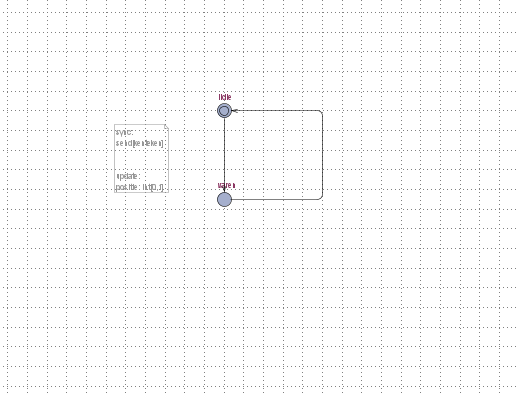
\includegraphics[width=8cm]{GeneralConsiderations/1mei/ship.png}
			%			\caption{}
			%			\label{fig:1a}
			%		\end{subfigure}
		%		\caption{Sluismodel 1 mei}
		%		\label{fig:1}
		%	\end{figure}
	%	
	%	
	%	
	%	
	%	\begin{figure}
		%		\centering
		%		\begin{subfigure}{0.45\linewidth}
			%			\includegraphics[width=8cm]{GeneralConsiderations/1mei/sluiskolk.png}
			%			\caption{}
			%			\label{fig:1a}
			%		\end{subfigure}\hfill
		%		\begin{subfigure}{0.45\linewidth}
			%			\includegraphics[width=8cm]{GeneralConsiderations/1mei/stoplicht.png}
			%			\caption{}
			%			\label{fig:1a}
			%		\end{subfigure}
		%		
		%		\begin{subfigure}{0.45\linewidth}
			%			
\includegraphics[width=8cm]{GeneralConsiderations/1mei/system.png}
			%			\caption{}
			%			\label{fig:1a}
			%		\end{subfigure}\hfill
		%		\begin{subfigure}{0.45\linewidth}
			%			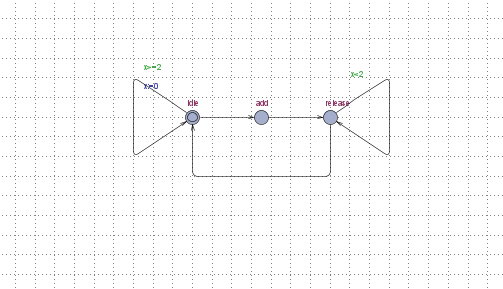
\includegraphics[width=8cm]{GeneralConsiderations/1mei/wCHTRIJ.png}
			%			\caption{}
			%			\label{fig:1a}
			%		\end{subfigure}
		%		\caption{Sluismodel 1 mei}
		%		\label{fig:1}
		%	\end{figure}
	%	%%%%%%%%%%%%%%%%%%%%%%%%%%%%%%%%%%%%%%%%%%%%%%%%%%%%%%%%%%%%%%%%%
	%	\newpage
	%	\subsection{Ontwerpen: 2 juni}
	%	
	%	
	%	
	%	\begin{figure}
		%		\centering
		%		\begin{subfigure}{0.45\linewidth}
			%			\includegraphics[width=8cm]{GeneralConsiderations/2juni/decl1.png}
			%			\caption{}
			%			\label{fig:1a}
			%		\end{subfigure}\hfill
		%		\begin{subfigure}{0.45\linewidth}
			%			\includegraphics[width=8cm]{GeneralConsiderations/2juni/decl1.png }
			%			\caption{}
			%			\label{fig:1a}
			%		\end{subfigure}
		%		
		%		\begin{subfigure}{0.45\linewidth}
			%			\includegraphics[width=8cm]{GeneralConsiderations/2juni/decl3.png }
			%			\caption{}
			%			\label{fig:1a}
			%		\end{subfigure}\hfill
		%		\begin{subfigure}{0.45\linewidth}
			%			\includegraphics[width=8cm]{GeneralConsiderations/2juni/gate.png }
			%			\caption{}
			%			\label{fig:1a}
			%		\end{subfigure}
		%		\caption{Sluismodel 2 juni}
		%		\label{fig:1}
		%	\end{figure}
	%	
	%	
	%	
	%	
	%	\begin{figure}
		%		\centering
		%		\begin{subfigure}{0.45\linewidth}
			%			\includegraphics[width=8cm]{GeneralConsiderations/2juni/main.png }
			%			\caption{}
			%			\label{fig:1a}
			%		\end{subfigure}\hfill
		%		\begin{subfigure}{0.45\linewidth}
			%			\includegraphics[width=8cm]{GeneralConsiderations/2juni/maincontroller.png }
			%			\caption{}
			%			\label{fig:1a}
			%		\end{subfigure}
		%		
		%		\begin{subfigure}{0.45\linewidth}
			%			\includegraphics[width=8cm]{GeneralConsiderations/2juni/pomp }
			%			\caption{}
			%			\label{fig:1a}
			%		\end{subfigure}\hfill
		%		\begin{subfigure}{0.45\linewidth}
			%			\includegraphics[width=8cm]{GeneralConsiderations/2juni/schip }
			%			\caption{}
			%			\label{fig:1a}
			%		\end{subfigure}
		%		\caption{Sluismodel 2 juni}
		%		\label{fig:1}
		%	\end{figure}
	%	
	%	
	%	
	%	
	%	\begin{figure}
		%		\centering
		%		\begin{subfigure}{0.45\linewidth}
			%			\includegraphics[width=8cm]{GeneralConsiderations/2juni/sensor }
			%			\caption{}
			%			\label{fig:1a}
			%		\end{subfigure}\hfill
		%		\begin{subfigure}{0.45\linewidth}
			%			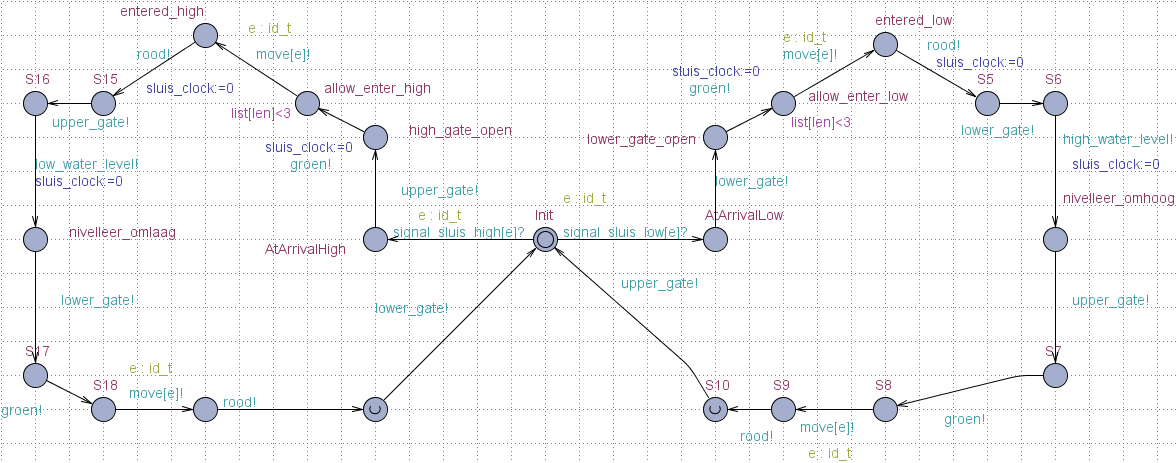
\includegraphics[width=8cm]{GeneralConsiderations/2juni/sluis }
			%			\caption{}
			%			\label{fig:1a}
			%		\end{subfigure}
		%		
		%		\begin{subfigure}{0.45\linewidth}
			%			\includegraphics[width=8cm]{GeneralConsiderations/2juni/stoplicht }
			%			\caption{}
			%			\label{fig:1a}
			%		\end{subfigure}\hfill
		%		\begin{subfigure}{0.45\linewidth}
			%			
\includegraphics[width=8cm]{GeneralConsiderations/2juni/system }
			%			\caption{}
			%			\label{fig:1a}
			%		\end{subfigure}
		%		\caption{Sluismodel 2 juni}
		%		\label{fig:1}
		%	\end{figure}
	%	%%%%%%%%%%%%%%%%%%%%%%%%%%%%%%%%%%%%%%%%%%%%%%%%%%%%%%%%%%%%%%%%%
	%	\newpage
	%	\subsection{Ontwerpen: 2 mei}
	%	
	%	
	%	
	%	
	%	\begin{figure}
		%		\centering
		%		\begin{subfigure}{0.45\linewidth}
			%			\includegraphics[width=8cm]{GeneralConsiderations/2mei/decl1.png}
			%			\caption{}
			%			\label{fig:1a}
			%		\end{subfigure}\hfill
		%		\begin{subfigure}{0.45\linewidth}
			%			\includegraphics[width=8cm]{GeneralConsiderations/2mei/decl2.png}
			%			\caption{}
			%			\label{fig:1a}
			%		\end{subfigure}
		%		
		%		\begin{subfigure}{0.45\linewidth}
			%			\includegraphics[width=8cm]{GeneralConsiderations/2mei/decl3.png}
			%			\caption{}
			%			\label{fig:1a}
			%		\end{subfigure}\hfill
		%		\begin{subfigure}{0.45\linewidth}
			%			\includegraphics[width=8cm]{GeneralConsiderations/2mei/gate.png}
			%			\caption{}
			%			\label{fig:1a}
			%		\end{subfigure}
		%		\caption{Sluismodel 2 mei}
		%		\label{fig:1}
		%	\end{figure}
	%	
	%	
	%	
	%	
	%	\begin{figure}
		%		\centering
		%		\begin{subfigure}{0.45\linewidth}
			%			\includegraphics[width=8cm]{GeneralConsiderations/2mei/main.png}
			%			\caption{}
			%			\label{fig:1a}
			%		\end{subfigure}\hfill
		%		\begin{subfigure}{0.45\linewidth}
			%			\includegraphics[width=8cm]{GeneralConsiderations/2mei/maincontroller.png}
			%			\caption{}
			%			\label{fig:1a}
			%		\end{subfigure}
		%		
		%		\begin{subfigure}{0.45\linewidth}
			%			\includegraphics[width=8cm]{GeneralConsiderations/2mei/pomp.png}
			%			\caption{}
			%			\label{fig:1a}
			%		\end{subfigure}\hfill
		%		\begin{subfigure}{0.45\linewidth}
			%			\includegraphics[width=8cm]{GeneralConsiderations/2mei/schip.png}
			%			\caption{}
			%			\label{fig:1a}
			%		\end{subfigure}
		%		\caption{Sluismodel 2 mei}
		%		\label{fig:1}
		%	\end{figure}
	%	
	%	
	%	
	%	
	%	
	%	\begin{figure}
		%		\centering
		%		\begin{subfigure}{0.45\linewidth}
			%			\includegraphics[width=8cm]{GeneralConsiderations/2mei/sensor.png}
			%			\caption{}
			%			\label{fig:1a}
			%		\end{subfigure}\hfill
		%		\begin{subfigure}{0.45\linewidth}
			%			\includegraphics[width=8cm]{GeneralConsiderations/2mei/sluiskolk.png}
			%			\caption{}
			%			\label{fig:1a}
			%		\end{subfigure}
		%		
		%		\begin{subfigure}{0.45\linewidth}
			%			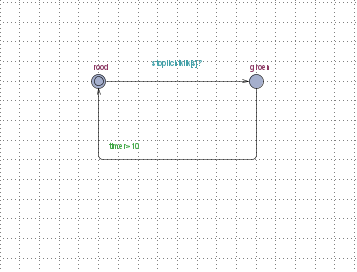
\includegraphics[width=8cm]{GeneralConsiderations/2mei/stoplight.png}
			%			\caption{}
			%			\label{fig:1a}
			%		\end{subfigure}\hfill
		%		\begin{subfigure}{0.45\linewidth}
			%			
\includegraphics[width=8cm]{GeneralConsiderations/2mei/system.png}
			%			\caption{}
			%			\label{fig:1a}
			%		\end{subfigure}
		%		\caption{Sluismodel 2 mei}
		%		\label{fig:1}
		%	\end{figure}
	%	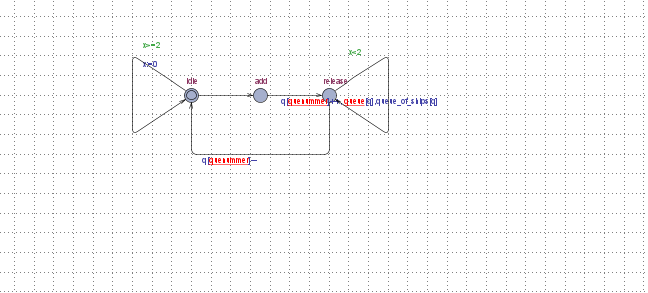
\includegraphics[width=8cm]{GeneralConsiderations/2mei/wachtrij.png}
	%	%%%%%%%%%%%%%%%%%%%%%%%%%%%%%%%%%%%%%%%%%%%%%%%%%%%%%%%%%%%%%%%%%
	%	\newpage
	%	\subsection{Ontwerpen:4 juli }
	%	
	%	
	%	
	%	\begin{figure}
		%		\centering
		%		\begin{subfigure}{0.45\linewidth}
			%			\includegraphics[width=8cm]{GeneralConsiderations/4juli/decl1.png}
			%			\caption{}
			%			\label{fig:1a}
			%		\end{subfigure}\hfill
		%		\begin{subfigure}{0.45\linewidth}
			%			\includegraphics[width=8cm]{GeneralConsiderations/4juli/decl2.png}
			%			\caption{}
			%			\label{fig:1a}
			%		\end{subfigure}
		%		
		%		\begin{subfigure}{0.45\linewidth}
			%			\includegraphics[width=8cm]{GeneralConsiderations/4juli/decl3.png}
			%			\caption{}
			%			\label{fig:1a}
			%		\end{subfigure}\hfill
		%		\begin{subfigure}{0.45\linewidth}
			%			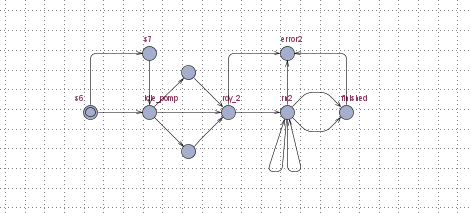
\includegraphics[width=8cm]{GeneralConsiderations/4juli/deurcontroller.png}
			%			\caption{}
			%			\label{fig:1a}
			%		\end{subfigure}
		%		\caption{Sluismodel 4 juli}
		%		\label{fig:1}
		%	\end{figure}
	%	
	%	
	%	
	%	
	%	
	%	
	%	
	%	
	%	
	%	\begin{figure}
		%		\centering
		%		\begin{subfigure}{0.45\linewidth}
			%			\includegraphics[width=8cm]{GeneralConsiderations/4juli/gate.png}
			%			\caption{}
			%			\label{fig:1a}
			%		\end{subfigure}\hfill
		%		\begin{subfigure}{0.45\linewidth}
			%			\includegraphics[width=8cm]{GeneralConsiderations/4juli/main.png}
			%			\caption{}
			%			\label{fig:1a}
			%		\end{subfigure}
		%		
		%		\begin{subfigure}{0.45\linewidth}
			%			\includegraphics[width=8cm]{GeneralConsiderations/4juli/manicontroller.png}
			%			\caption{}
			%			\label{fig:1a}
			%		\end{subfigure}\hfill
		%		\begin{subfigure}{0.45\linewidth}
			%			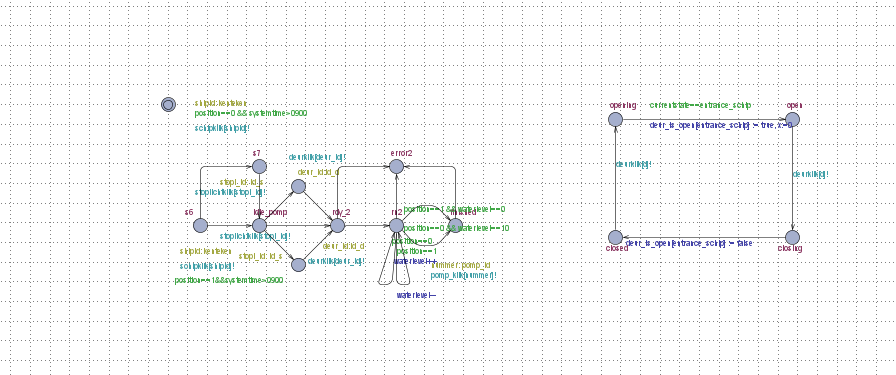
\includegraphics[width=8cm]{GeneralConsiderations/4juli/newdeur.png}
			%			\caption{}
			%			\label{fig:1a}
			%		\end{subfigure}
		%		\caption{Sluismodel 4 juli}
		%		\label{fig:1}
		%	\end{figure}
	%	
	%	
	%	
	%	
	%	
	%	\begin{figure}
		%		\centering
		%		\begin{subfigure}{0.45\linewidth}
			%			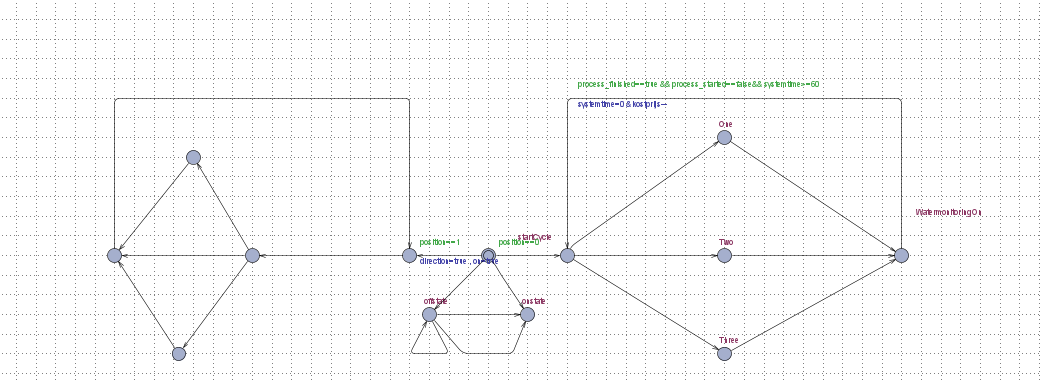
\includegraphics[width=8cm]{GeneralConsiderations/4juli/newmain.png}
			%			\caption{}
			%			\label{fig:1a}
			%		\end{subfigure}\hfill
		%		\begin{subfigure}{0.45\linewidth}
			%			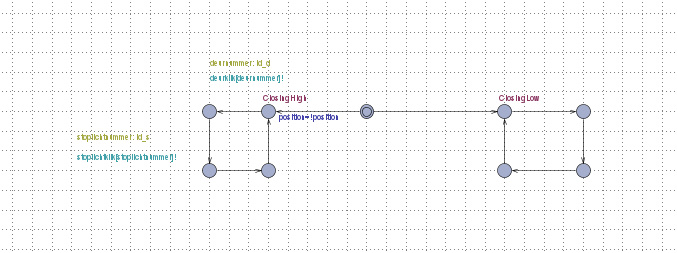
\includegraphics[width=8cm]{GeneralConsiderations/4juli/newmainclosing.png}
			%			\caption{}
			%			\label{fig:1a}
			%		\end{subfigure}
		%		
		%		\begin{subfigure}{0.45\linewidth}
			%			\includegraphics[width=8cm]{GeneralConsiderations/4juli/newmainopening.png}
			%			\caption{}
			%			\label{fig:1a}
			%		\end{subfigure}\hfill
		%		\begin{subfigure}{0.45\linewidth}
			%			\includegraphics[width=8cm]{GeneralConsiderations/4juli/newpomp.png}
			%			\caption{}
			%			\label{fig:1a}
			%		\end{subfigure}
		%		\caption{Sluismodel 4 juli}
		%		\label{fig:1}
		%	\end{figure}
	%	
	%	
	%	
	%	
	%	
	%	\begin{figure}
		%		\centering
		%		\begin{subfigure}{0.45\linewidth}
			%			\includegraphics[width=8cm]{GeneralConsiderations/4juli/priorityqueue.png} 
			%			\caption{}
			%			\label{fig:1a}
			%		\end{subfigure}\hfill
		%		\begin{subfigure}{0.45\linewidth}
			%			\includegraphics[width=8cm]{GeneralConsiderations/4juli/request.png}
			%			\caption{}
			%			\label{fig:1a}
			%		\end{subfigure}
		%		
		%		\begin{subfigure}{0.45\linewidth}
			%			\includegraphics[width=8cm]{GeneralConsiderations/4juli/schip.png}
			%			\caption{}
			%			\label{fig:1a}
			%		\end{subfigure}\hfill
		%		\begin{subfigure}{0.45\linewidth}
			%			\includegraphics[width=8cm]{GeneralConsiderations/4juli/sensor.png}
			%			\caption{}
			%			\label{fig:1a}
			%		\end{subfigure}
		%		\caption{Sluismodel 4 juli}
		%		\label{fig:1}
		%	\end{figure}
	%	
	%	
	%	
	%	
	%	\begin{figure}
		%		\centering
		%		\begin{subfigure}{0.45\linewidth}
			%			\includegraphics[width=8cm]{GeneralConsiderations/4juli/sluis.png}
			%			\caption{}
			%			\label{fig:1a}
			%		\end{subfigure}\hfill
		%		\begin{subfigure}{0.45\linewidth}
			%			\includegraphics[width=8cm]{GeneralConsiderations/4juli/stoplight.png}
			%			\caption{}
			%			\label{fig:1a}
			%		\end{subfigure}
		%		
		%		\begin{subfigure}{0.45\linewidth}
			%			\includegraphics[width=8cm]{GeneralConsiderations/4juli/system.png}
			%			\caption{}
			%			\label{fig:1a}
			%		\end{subfigure}\hfill
		%		\begin{subfigure}{0.45\linewidth}
			%			\includegraphics[width=8cm]{GeneralConsiderations/4juli/waterlevelsensingHigh.png}
			%			\caption{}
			%			\label{fig:1a}
			%		\end{subfigure}
		%		\caption{Sluismodel van 4 juli}
		%		\label{fig:1}
		%	\end{figure}
	%	%%%%%%%%%%%%%%%%%%%%%%%%%%%%%%%%%%%%%%%%%%%%%%%%%%%%%%%%%%%%%%%%%
	%	\newpage
	%	
	%	\includegraphics[width=8cm]{GeneralConsiderations/5mei}
	%	%%%%%%%%%%%%%%%%%%%%%%%%%%%%%%%%%%%%%%%%%%%%%%%%%%%%%%%%%%%%%%%%%
	%	
	%	\newpage
	%	\subsection{Ontwerpen: 6 juni}
	%	
	%	
	%	\begin{figure}
		%		\centering
		%		\begin{subfigure}{0.45\linewidth}
			%			\includegraphics[width=8cm]{GeneralConsiderations/6juni/decl1.png}
			%			\caption{}
			%			\label{fig:1a}
			%		\end{subfigure}\hfill
		%		\begin{subfigure}{0.45\linewidth}
			%			\includegraphics[width=8cm]{GeneralConsiderations/6juni/decl2.png}
			%			\caption{}
			%			\label{fig:1a}
			%		\end{subfigure}
		%		
		%		\begin{subfigure}{0.45\linewidth}
			%			\includegraphics[width=8cm]{GeneralConsiderations/6juni/decl3.png}
			%			\caption{}
			%			\label{fig:1a}
			%		\end{subfigure}\hfill
		%		\begin{subfigure}{0.45\linewidth}
			%			\includegraphics[width=8cm]{GeneralConsiderations/6juni/ensor.png}
			%			\caption{}
			%			\label{fig:1a}
			%		\end{subfigure}
		%		\caption{Sluismodl van 6 juni}
		%		\label{fig:1}
		%	\end{figure}
	%	
	%	
	%	
	%	
	%	\begin{figure}
		%		\centering
		%		\begin{subfigure}{0.45\linewidth}
			%			\includegraphics[width=8cm]{GeneralConsiderations/6juni/gate.png}
			%			\caption{}
			%			\label{fig:1a}
			%		\end{subfigure}\hfill
		%		\begin{subfigure}{0.45\linewidth}
			%			\includegraphics[width=8cm]{GeneralConsiderations/6juni/main.png}
			%			\caption{}
			%			\label{fig:1a}
			%		\end{subfigure}
		%		
		%		\begin{subfigure}{0.45\linewidth}
			%			\includegraphics[width=8cm]{GeneralConsiderations/6juni/maincontroller.png}
			%			\caption{}
			%			\label{fig:1a}
			%		\end{subfigure}\hfill
		%		\begin{subfigure}{0.45\linewidth}
			%			\includegraphics[width=8cm]{GeneralConsiderations/6juni/pomp.png}
			%			\caption{}
			%			\label{fig:1a}
			%		\end{subfigure}
		%		\caption{Sluismodel 6 juni}
		%		\label{fig:1}
		%	\end{figure}
	%	
	%	
	%	
	%	
	%	\begin{figure}
		%		\centering
		%		\begin{subfigure}{0.45\linewidth}
			%			\includegraphics[width=8cm]{GeneralConsiderations/6juni/ship.png}
			%			\caption{}
			%			\label{fig:1a}
			%		\end{subfigure}\hfill
		%		\begin{subfigure}{0.45\linewidth}
			%			\includegraphics[width=8cm]{GeneralConsiderations/6juni/sluis.png}
			%			\caption{}
			%			\label{fig:1a}
			%		\end{subfigure}
		%		
		%		\begin{subfigure}{0.45\linewidth}
			%			\includegraphics[width=8cm]{GeneralConsiderations/6juni/stoplight.png}
			%			\caption{}
			%			\label{fig:1a}
			%		\end{subfigure}\hfill
		%		\begin{subfigure}{0.45\linewidth}
			%			\includegraphics[width=8cm]{GeneralConsiderations/6juni/system.png}
			%			\caption{}
			%			\label{fig:1a}
			%		\end{subfigure}
		%		\caption{Sluismodel 6 juni}
		%		\label{fig:1}
		%	\end{figure}
	%	%%%%%%%%%%%%%%%%%%%%%%%%%%%%%%%%%%%%%%%%%%%%%%%%%%%%%%%%%%%%%%%%%
	%	\newpage
	%	\subsection{Ontwerpen: 8 juni }
	%	
	%	
	%	
	%	
	%	\begin{figure}
		%		\centering
		%		\begin{subfigure}{0.45\linewidth}
			%			\includegraphics[width=8cm]{GeneralConsiderations/8juni/decl1.png}
			%			\caption{}
			%			\label{fig:1a}
			%		\end{subfigure}\hfill
		%		\begin{subfigure}{0.45\linewidth}
			%			\includegraphics[width=8cm]{GeneralConsiderations/8juni/decl2.png}
			%			\caption{}
			%			\label{fig:1a}
			%		\end{subfigure}
		%		
		%		\begin{subfigure}{0.45\linewidth}
			%			\includegraphics[width=8cm]{GeneralConsiderations/8juni/decl3.png}
			%			\caption{}
			%			\label{fig:1a}
			%		\end{subfigure}\hfill
		%		\begin{subfigure}{0.45\linewidth}
			%			\includegraphics[width=8cm]{GeneralConsiderations/8juni/decl4.png}
			%			\caption{}
			%			\label{fig:1a}
			%		\end{subfigure}
		%		\caption{Sluismodel 8 juni}
		%		\label{fig:1}
		%	\end{figure}
	%	
	%	
	%	
	%	
	%	\begin{figure}
		%		\centering
		%		\begin{subfigure}{0.45\linewidth}
			%			\includegraphics[width=8cm]{GeneralConsiderations/8juni/gate.png}
			%			\caption{}
			%			\label{fig:1a}
			%		\end{subfigure}\hfill
		%		\begin{subfigure}{0.45\linewidth}
			%			\includegraphics[width=8cm]{GeneralConsiderations/8juni/main.png}
			%			\caption{}
			%			\label{fig:1a}
			%		\end{subfigure}
		%		
		%		\begin{subfigure}{0.45\linewidth}
			%			\includegraphics[width=8cm]{GeneralConsiderations/8juni/maincontroller.png}
			%			\caption{}
			%			\label{fig:1a}
			%		\end{subfigure}\hfill
		%		\begin{subfigure}{0.45\linewidth}
			%			\includegraphics[width=8cm]{GeneralConsiderations/8juni/pomp.png}
			%			\caption{}
			%			\label{fig:1a}
			%		\end{subfigure}
		%		\caption{Sluismodel 8 juni}
		%		\label{fig:1}
		%	\end{figure}
	%	
	%	
	%	
	%	
	%	\begin{figure}
		%		\centering
		%		\begin{subfigure}{0.45\linewidth}
			%			\includegraphics[width=8cm]{GeneralConsiderations/8juni/schip.png}
			%			\caption{}
			%			\label{fig:1a}
			%		\end{subfigure}\hfill
		%		\begin{subfigure}{0.45\linewidth}
			%			\includegraphics[width=8cm]{GeneralConsiderations/8juni/sensor.png}
			%			\caption{}
			%			\label{fig:1a}
			%		\end{subfigure}
		%		
		%		\begin{subfigure}{0.45\linewidth}
			%			\includegraphics[width=8cm]{GeneralConsiderations/8juni/sluis.png}
			%			\caption{}
			%			\label{fig:1a}
			%		\end{subfigure}\hfill
		%		\begin{subfigure}{0.45\linewidth}
			%			\includegraphics[width=8cm]{GeneralConsiderations/8juni/stoplicht.png}
			%			\caption{}
			%			\label{fig:1a}
			%		\end{subfigure}
		%		\caption{Sluismodel 8 juni}
		%		\label{fig:1}
		%	\end{figure}
	%	\includegraphics[width=8cm]{GeneralConsiderations/8juni/systeem.png}3
	%	%%%%%%%%%%%%%%%%%%%%%%%%%%%%%%%%%%%%%%%%%%%%%%%%%%%%%%%%%%%%%%%%%
	%	\newpage
	%	\subsection{Ontwerpen: 10 april}
	%	
	%	
	%	
	%	
	%	\begin{figure}
		%		\centering
		%		\begin{subfigure}{0.45\linewidth}
			%			\includegraphics[width=8cm]{GeneralConsiderations/10april/aanvoer.png}
			%			\caption{}
			%			\label{fig:1a}
			%		\end{subfigure}\hfill
		%		\begin{subfigure}{0.45\linewidth}
			%			\includegraphics[width=8cm]{GeneralConsiderations/10april/afvoer.png}
			%			\caption{}
			%			\label{fig:1a}
			%		\end{subfigure}
		%		
		%		\begin{subfigure}{0.45\linewidth}
			%			\includegraphics[width=8cm]{GeneralConsiderations/10april/controller.png}
			%			\caption{}
			%			\label{fig:1a}
			%		\end{subfigure}\hfill
		%		\begin{subfigure}{0.45\linewidth}
			%			\includegraphics[width=8cm]{GeneralConsiderations/10april/decl1.png}
			%			\caption{}
			%			\label{fig:1a}
			%		\end{subfigure}
		%		\caption{Sluismodel 10 april}
		%		\label{fig:1}
		%	\end{figure}
	%	
	%	
	%	
	%	
	%	\begin{figure}
		%		\centering
		%		\begin{subfigure}{0.45\linewidth}
			%			\includegraphics[width=8cm]{GeneralConsiderations/10april/pomp.png} 
			%			\caption{}
			%			\label{fig:1a}
			%		\end{subfigure}\hfill
		%		\begin{subfigure}{0.45\linewidth}
			%			\includegraphics[width=8cm]{GeneralConsiderations/10april/schip.png}
			%			\caption{}
			%			\label{fig:1a}
			%		\end{subfigure}
		%		
		%		\begin{subfigure}{0.45\linewidth}
			%			\includegraphics[width=8cm]{GeneralConsiderations/10april/sluisdeur.png}
			%			\caption{}
			%			\label{fig:1a}
			%		\end{subfigure}\hfill
		%		\begin{subfigure}{0.45\linewidth}
			%			\includegraphics[width=8cm]{GeneralConsiderations/10april/sluiskant.png}
			%			\caption{}
			%			\label{fig:1a}
			%		\end{subfigure}
		%		\caption{Sluismodel 10 april}
		%		\label{fig:1}
		%	\end{figure}
	%	
	%	
	%	\begin{figure}
		%		\centering
		%		\begin{subfigure}{0.45\linewidth}
			%			\includegraphics[width=8cm]{GeneralConsiderations/10april/stoplicht.png}
			%			\caption{}
			%			\label{fig:1a}
			%		\end{subfigure}\hfill
		%		\begin{subfigure}{0.45\linewidth}
			%			\includegraphics[width=8cm]{GeneralConsiderations/10april/systeem.png}
			%			\caption{}
			%			\label{fig:1a}
			%		\end{subfigure}
		%	\end{figure}
	%	
	%	%%%%%%%%%%%%%%%%%%%%%%%%%%%%%%%%%%%%%%%%%%%%%%%%%%%%%%%%%%%%%%%%%
	%	\newpage
	%	\subsection{Ontwerpen: 12 juni}
	%	
	%	
	%	
	%	
	%	\begin{figure}
		%		\centering
		%		\begin{subfigure}{0.45\linewidth}
			%			\includegraphics[width=8cm]{GeneralConsiderations/12juni/decl1.png}
			%			\caption{}
			%			\label{fig:1a}
			%		\end{subfigure}\hfill
		%		\begin{subfigure}{0.45\linewidth}
			%			\includegraphics[width=8cm]{GeneralConsiderations/12juni/decl2.png}
			%			\caption{}
			%			\label{fig:1a}
			%		\end{subfigure}
		%		
		%		\begin{subfigure}{0.45\linewidth}
			%			\includegraphics[width=8cm]{GeneralConsiderations/12juni/decl3.png}
			%			\caption{}
			%			\label{fig:1a}
			%		\end{subfigure}\hfill
		%		\begin{subfigure}{0.45\linewidth}
			%			\includegraphics[width=8cm]{GeneralConsiderations/12juni/deurcontroller.png}
			%			\caption{}
			%			\label{fig:1a}
			%		\end{subfigure}
		%		\caption{Sluismodel 12 juni}
		%		\label{fig:1}
		%	\end{figure}
	%	\begin{figure}
		%		\centering
		%		\begin{subfigure}{0.45\linewidth}
			%			\includegraphics[width=8cm]{GeneralConsiderations/12juni/gate.png}
			%			\caption{}
			%			\label{fig:1a}
			%		\end{subfigure}\hfill
		%		\begin{subfigure}{0.45\linewidth}
			%			\includegraphics[width=8cm]{GeneralConsiderations/12juni/main.png}
			%			\caption{}
			%			\label{fig:1a}
			%		\end{subfigure}
		%		
		%		\begin{subfigure}{0.45\linewidth}
			%			\includegraphics[width=8cm]{GeneralConsiderations/12juni/maincontroller.png}
			%			\caption{}
			%			\label{fig:1a}
			%		\end{subfigure}\hfill
		%		\begin{subfigure}{0.45\linewidth}
			%			\includegraphics[width=8cm]{GeneralConsiderations/12juni/newdeur.png}
			%			\caption{}
			%			\label{fig:1a}
			%		\end{subfigure}
		%		\caption{Sluismodel 12 juni}
		%		\label{fig:1}
		%	\end{figure}
	%	\begin{figure}
		%		\centering
		%		\begin{subfigure}{0.45\linewidth}
			%			\includegraphics[width=8cm]{GeneralConsiderations/12juni/newmaincontroller.png}
			%			\caption{}
			%			\label{fig:1a}
			%		\end{subfigure}\hfill
		%		\begin{subfigure}{0.45\linewidth}
			%			\includegraphics[width=8cm]{GeneralConsiderations/12juni/newmainclosingproc.png}
			%			\caption{}
			%			\label{fig:1a}
			%		\end{subfigure}
		%		
		%		\begin{subfigure}{0.45\linewidth}
			%			\includegraphics[width=8cm]{GeneralConsiderations/12juni/newmainOpeningProc.png}
			%			\caption{}
			%			\label{fig:1a}
			%		\end{subfigure}\hfill
		%		\begin{subfigure}{0.45\linewidth}
			%			\includegraphics[width=8cm]{GeneralConsiderations/12juni/newpomp.png}
			%			\caption{}
			%			\label{fig:1a}
			%		\end{subfigure}
		%		\caption{Sluismodel 12 juni}
		%		\label{fig:1}
		%	\end{figure}
	%	\begin{figure}
		%		\centering
		%		\begin{subfigure}{0.45\linewidth}
			%			\includegraphics[width=8cm]{GeneralConsiderations/12juni/pomp.png}
			%			\caption{}
			%			\label{fig:1a}
			%		\end{subfigure}\hfill
		%		\begin{subfigure}{0.45\linewidth}
			%			\includegraphics[width=8cm]{GeneralConsiderations/12juni/priorityqueue.png}
			%			\caption{}
			%			\label{fig:1a}
			%		\end{subfigure}
		%		
		%		\begin{subfigure}{0.45\linewidth}
			%			\includegraphics[width=8cm]{GeneralConsiderations/12juni/request.png}
			%			\caption{}
			%			\label{fig:1a}
			%		\end{subfigure}\hfill
		%		\begin{subfigure}{0.45\linewidth}
			%			\includegraphics[width=8cm]{GeneralConsiderations/12juni/schip.png}
			%			\caption{}
			%			\label{fig:1a}
			%		\end{subfigure}
		%		\caption{Sluismodel 12 juni}
		%		\label{fig:1}
		%	\end{figure}
	%	\begin{figure}
		%		\centering
		%		\begin{subfigure}{0.45\linewidth}
			%			\includegraphics[width=8cm]{GeneralConsiderations/12juni/sensor.png}
			%			\caption{}
			%			\label{fig:1a}
			%		\end{subfigure}\hfill
		%		\begin{subfigure}{0.45\linewidth}
			%			\includegraphics[width=8cm]{GeneralConsiderations/12juni/sluis.png}
			%			\caption{}
			%			\label{fig:1a}
			%		\end{subfigure}
		%		
		%		\begin{subfigure}{0.45\linewidth}
			%			\includegraphics[width=8cm]{GeneralConsiderations/12juni/stoplicht.png}
			%			\caption{}
			%			\label{fig:1a}
			%		\end{subfigure}\hfill
		%		\begin{subfigure}{0.45\linewidth}
			%			\includegraphics[width=8cm]{GeneralConsiderations/12juni/system.png}
			%			\caption{}
			%			\label{fig:1a}
			%		\end{subfigure}
		%		\caption{Sluismodel 12 juni}
		%		\label{fig:1}
		%	\end{figure}
	%	
	%	\begin{figure}
		%		\centering
		%		\begin{subfigure}{0.45\linewidth}
			%			\includegraphics[width=8cm]{GeneralConsiderations/12juni/waterlevelensorhigh.png}
			%			\caption{}
			%			\label{fig:1a}
			%		\end{subfigure}\hfill
		%		\begin{subfigure}{0.45\linewidth}
			%			\includegraphics[width=8cm]{GeneralConsiderations/12juni/decl1.png}
			%			\caption{}
			%			\label{fig:1a}
			%		\end{subfigure}
		%	\end{figure}
	%	%%%%%%%%%%%%%%%%%%%%%%%%%%%%%%%%%%%%%%%%%%%%%%%%%%%%%%%%%%%%%%%%%
	%	\newpage
	%	\subsection{Ontwerpen: 12 september}
	%	\includegraphics[width=8cm]{GeneralConsiderations/12september/maincontroller.png}
	%	%%%%%%%%%%%%%%%%%%%%%%%%%%%%%%%%%%%%%%%%%%%%%%%%%%%%%%%%%%%%%%%%%]
	%	\newpage
	%	\subsection{Ontwerpen: 13 april}
	%	\begin{figure}
		%		\centering
		%		\begin{subfigure}{0.45\linewidth}
			%			\includegraphics[width=8cm]{GeneralConsiderations/13april/aanvoer.png}
			%			\caption{}
			%			\label{fig:1a}
			%		\end{subfigure}\hfill
		%		\begin{subfigure}{0.45\linewidth}
			%			\includegraphics[width=8cm]{GeneralConsiderations/13april/afvoer.png}
			%			\caption{}
			%			\label{fig:1a}
			%		\end{subfigure}
		%		
		%		\begin{subfigure}{0.45\linewidth}
			%			\includegraphics[width=8cm]{GeneralConsiderations/13april/controller.png}
			%			\caption{}
			%			\label{fig:1a}
			%		\end{subfigure}\hfill
		%		\begin{subfigure}{0.45\linewidth}
			%			\includegraphics[width=8cm]{GeneralConsiderations/13april/decl.png}
			%			\caption{}
			%			\label{fig:1a}
			%		\end{subfigure}
		%		\caption{Sluismodel 13 april}
		%		\label{fig:1}
		%	\end{figure}
	%	\begin{figure}
		%		\centering
		%		\begin{subfigure}{0.45\linewidth}
			%			\includegraphics[width=8cm]{GeneralConsiderations/13april/pomp.png}
			%			\caption{}
			%			\label{fig:1a}
			%		\end{subfigure}\hfill
		%		\begin{subfigure}{0.45\linewidth}
			%			\includegraphics[width=8cm]{GeneralConsiderations/13april/schip.png}
			%			\caption{}
			%			\label{fig:1a}
			%		\end{subfigure}
		%		
		%		\begin{subfigure}{0.45\linewidth}
			%			\includegraphics[width=8cm]{GeneralConsiderations/13april/sluis.png}
			%			\caption{}
			%			\label{fig:1a}
			%		\end{subfigure}\hfill
		%		\begin{subfigure}{0.45\linewidth}
			%			\includegraphics[width=8cm]{GeneralConsiderations/13april/sluisdeur.png}
			%			\caption{}
			%			\label{fig:1a}
			%		\end{subfigure}
		%		\caption{Sluismodel 13 april}
		%		\label{fig:1}
		%	\end{figure}
	%	
	%	\begin{figure}
		%		\centering
		%		\begin{subfigure}{0.45\linewidth}
			%			\includegraphics[width=8cm]{GeneralConsiderations/13april/stoplicht.png}
			%			\caption{}
			%			\label{fig:1a}
			%		\end{subfigure}\hfill
		%		\begin{subfigure}{0.45\linewidth}
			%			\includegraphics[width=8cm]{GeneralConsiderations/13april/system.png}
			%			\caption{}
			%			\label{fig:1a}
			%		\end{subfigure}
		%	\end{figure}
	%	%%%%%%%%%%%%%%%%%%%%%%%%%%%%%%%%%%%%%%%%%%%%%%%%%%%%%%%%%%%%%%%%%
	%	\newpage
	%	\subsection{Ontwerpen: 13 juni}
	%	\begin{figure}
		%		\centering
		%		\begin{subfigure}{0.45\linewidth}
			%			\includegraphics[width=8cm]{GeneralConsiderations/13juni/versie1/decl1.png}
			%			\caption{}
			%			\label{fig:1a}
			%		\end{subfigure}\hfill
		%		\begin{subfigure}{0.45\linewidth}
			%			\includegraphics[width=8cm]{GeneralConsiderations/13juni/versie1/decl2.png}
			%			\caption{}
			%			\label{fig:1a}
			%		\end{subfigure}
		%		
		%		\begin{subfigure}{0.45\linewidth}
			%			\includegraphics[width=8cm]{GeneralConsiderations/13juni/versie1/decl3.png}
			%			\caption{}
			%			\label{fig:1a}
			%		\end{subfigure}\hfill
		%		\begin{subfigure}{0.45\linewidth}
			%			\includegraphics[width=8cm]{GeneralConsiderations/13juni/versie1/deurcontroller.png}
			%			\caption{}
			%			\label{fig:1a}
			%		\end{subfigure}
		%		\caption{Sluismodel 13 juni versie 1}
		%		\label{fig:1}
		%	\end{figure}
	%	
	%	\begin{figure}
		%		\centering
		%		\begin{subfigure}{0.45\linewidth}
			%			\includegraphics[width=8cm]{GeneralConsiderations/13juni/versie1/gate.png}
			%			\caption{}
			%			\label{fig:1a}
			%		\end{subfigure}\hfill
		%		\begin{subfigure}{0.45\linewidth}
			%			\includegraphics[width=8cm]{GeneralConsiderations/13juni/versie1/main.png}
			%			\caption{}
			%			\label{fig:1a}
			%		\end{subfigure}
		%		
		%		\begin{subfigure}{0.45\linewidth}
			%			\includegraphics[width=8cm]{GeneralConsiderations/13juni/versie1/maincontroller.png}
			%			\caption{}
			%			\label{fig:1a}
			%		\end{subfigure}\hfill
		%		\begin{subfigure}{0.45\linewidth}
			%			\includegraphics[width=8cm]{GeneralConsiderations/13juni/versie1/main.png}
			%			\caption{}
			%			\label{fig:1a}
			%		\end{subfigure}
		%		\caption{Sluismodel 13 juni versie 1}
		%		\label{fig:1}
		%	\end{figure}
	%	
	%	\begin{figure}
		%		\centering
		%		\begin{subfigure}{0.45\linewidth}
			%			\includegraphics[width=8cm]{GeneralConsiderations/13juni/versie1/newdeur.png}
			%			\caption{}
			%			\label{fig:1a}
			%		\end{subfigure}\hfill
		%		\begin{subfigure}{0.45\linewidth}
			%			\includegraphics[width=8cm]{GeneralConsiderations/13juni/versie1/newmain.png}
			%			\caption{}
			%			\label{fig:1a}
			%		\end{subfigure}
		%		
		%		\begin{subfigure}{0.45\linewidth}
			%			\includegraphics[width=8cm]{GeneralConsiderations/13juni/versie1/newmainClosingProc.png}
			%			\caption{}
			%			\label{fig:1a}
			%		\end{subfigure}\hfill
		%		\begin{subfigure}{0.45\linewidth}
			%			\includegraphics[width=8cm]{GeneralConsiderations/13juni/versie1/newmainopeningProc.png}
			%			\caption{}
			%			\label{fig:1a}
			%		\end{subfigure}
		%		\caption{Sluismodel 13 juni versie 1}
		%		\label{fig:1}
		%	\end{figure}
	%	
	%	\begin{figure}
		%		\centering
		%		\begin{subfigure}{0.45\linewidth}
			%			\includegraphics[width=8cm]{GeneralConsiderations/13juni/versie1/pomp.png}
			%			\caption{}
			%			\label{fig:1a}
			%		\end{subfigure}\hfill
		%		\begin{subfigure}{0.45\linewidth}
			%			\includegraphics[width=8cm]{GeneralConsiderations/13juni/versie1/priorityqueue.png}
			%			\caption{}
			%			\label{fig:1a}
			%		\end{subfigure}
		%		
		%		\begin{subfigure}{0.45\linewidth}
			%			\includegraphics[width=8cm]{GeneralConsiderations/13juni/versie1/request.png}
			%			\caption{}
			%			\label{fig:1a}
			%		\end{subfigure}\hfill
		%		\begin{subfigure}{0.45\linewidth}
			%			\includegraphics[width=8cm]{GeneralConsiderations/13juni/versie1/sensor.png}
			%			\caption{}
			%			\label{fig:1a}
			%		\end{subfigure}
		%		\caption{Sluismodel 13 juni versie 1}
		%		\label{fig:1}
		%	\end{figure}
	%	
	%	
	%	\begin{figure}
		%		\centering
		%		\begin{subfigure}{0.45\linewidth}
			%			\includegraphics[width=8cm]{GeneralConsiderations/13juni/versie1/stolight.png}
			%			\caption{}
			%			\label{fig:1a}
			%		\end{subfigure}\hfill
		%		\begin{subfigure}{0.45\linewidth}
			%			\includegraphics[width=8cm]{GeneralConsiderations/13juni/versie1/wterlevelsensorHight.png}
			%			\caption{}
			%			\label{fig:1a}
			%		\end{subfigure}
		%	\end{figure}
	%	
	%	\includegraphics[width=8cm]{GeneralConsiderations/13juni/versie1/system.png}
	%	
	%	
	%	%    \includegraphics[width=8cm]{GeneralConsiderations/13juni/versie2/decl1.png}
	%	%%%%%%%%%%%%%%%%%%%%%%%%%%%%%%%%%%%%%%%%%%%%%%%%%%%%%%%%%%%%%%%%%
	%	\newpage
	%	\subsection{Ontwerpen: 15 april}
	%	\begin{figure}
		%		\centering
		%		\begin{subfigure}{0.45\linewidth}
			%			\includegraphics[width=8cm]{GeneralConsiderations/15april/versie1/aanvoer.png}
			%			\caption{}
			%			\label{fig:1a}
			%		\end{subfigure}\hfill
		%		\begin{subfigure}{0.45\linewidth}
			%			\includegraphics[width=8cm]{GeneralConsiderations/15april/versie1/afvoer.png}
			%			\caption{}
			%			\label{fig:1a}
			%		\end{subfigure}
		%		
		%		\begin{subfigure}{0.45\linewidth}
			%			\includegraphics[width=8cm]{GeneralConsiderations/15april/versie1/controller.png}
			%			\caption{}
			%			\label{fig:1a}
			%		\end{subfigure}\hfill
		%		\begin{subfigure}{0.45\linewidth}
			%			\includegraphics[width=8cm]{GeneralConsiderations/15april/versie1/decl.png}
			%			\caption{}
			%			\label{fig:1a}
			%		\end{subfigure}
		%		\caption{Sluismodel 15 april versie 1}
		%		\label{fig:1}
		%	\end{figure}
	%	
	%	\begin{figure}
		%		\centering
		%		\begin{subfigure}{0.45\linewidth}
			%			\includegraphics[width=8cm]{GeneralConsiderations/15april/versie1/pomp.png}
			%			\caption{}
			%			\label{fig:1a}
			%		\end{subfigure}\hfill
		%		\begin{subfigure}{0.45\linewidth}
			%			\includegraphics[width=8cm]{GeneralConsiderations/15april/versie1/schip.png}
			%			\caption{}
			%			\label{fig:1a}
			%		\end{subfigure}
		%		
		%		\begin{subfigure}{0.45\linewidth}
			%			\includegraphics[width=8cm]{GeneralConsiderations/15april/versie1/sluis.png}
			%			\caption{}
			%			\label{fig:1a}
			%		\end{subfigure}\hfill
		%		\begin{subfigure}{0.45\linewidth}
			%			\includegraphics[width=8cm]{GeneralConsiderations/15april/versie1/sluisdeur.png}
			%			\caption{}
			%			\label{fig:1a}
			%		\end{subfigure}
		%		\caption{Sluismodel 15 april versie 1}
		%		\label{fig:1}
		%	\end{figure}
	%	
	%	
	%	\begin{figure}
		%		\centering
		%		\begin{subfigure}{0.45\linewidth}
			%			\includegraphics[width=8cm]{GeneralConsiderations/15april/versie1/stoplicht.png}
			%			\caption{}
			%			\label{fig:1a}
			%		\end{subfigure}\hfill
		%		\begin{subfigure}{0.45\linewidth}
			%			\includegraphics[width=8cm]{GeneralConsiderations/15april/versie1/system.png}
			%			\caption{}
			%			\label{fig:1a}
			%		\end{subfigure}
		%	\end{figure}
	%	
	%	
	%	\includegraphics[width=8cm]{GeneralConsiderations/15april/versie2/aanvoer.png}
	%	%%%%%%%%%%%%%%%%%%%%%%%%%%%%%%%%%%%%%%%%%%%%%%%%%%%%%%%%%%%%%%%%%
	%	\newpage
	%	\subsection{Ontwerpen:16 juli }
	%	\begin{figure}
		%		\centering
		%		\begin{subfigure}{0.45\linewidth}
			%			\includegraphics[width=8cm]{GeneralConsiderations/16juli/closingproc.png}
			%			\caption{}
			%			\label{fig:1a}
			%		\end{subfigure}\hfill
		%		\begin{subfigure}{0.45\linewidth}
			%			\includegraphics[width=8cm]{GeneralConsiderations/16juli/decl1.png}
			%			\caption{}
			%			\label{fig:1a}
			%		\end{subfigure}
		%		
		%		\begin{subfigure}{0.45\linewidth}
			%			\includegraphics[width=8cm]{GeneralConsiderations/16juli/decl2.png}
			%			\caption{}
			%			\label{fig:1a}
			%		\end{subfigure}\hfill
		%		\begin{subfigure}{0.45\linewidth}
			%			\includegraphics[width=8cm]{GeneralConsiderations/16juli/decl3.png}
			%			\caption{}
			%			\label{fig:1a}
			%		\end{subfigure}
		%		\caption{Sluismodel 16 juli}
		%		\label{fig:1}
		%	\end{figure}
	%	
	%	\begin{figure}
		%		\centering
		%		\begin{subfigure}{0.45\linewidth}
			%			\includegraphics[width=8cm]{GeneralConsiderations/16juli/deur.png}
			%			\caption{}
			%			\label{fig:1a}
			%		\end{subfigure}\hfill
		%		\begin{subfigure}{0.45\linewidth}
			%			\includegraphics[width=8cm]{GeneralConsiderations/16juli/maincontroller.png}
			%			\caption{}
			%			\label{fig:1a}
			%		\end{subfigure}
		%		
		%		\begin{subfigure}{0.45\linewidth}
			%			\includegraphics[width=8cm]{GeneralConsiderations/16juli/error.png}
			%			\caption{}
			%			\label{fig:1a}
			%		\end{subfigure}\hfill
		%		\begin{subfigure}{0.45\linewidth}
			%			\includegraphics[width=8cm]{GeneralConsiderations/16juli/openingproc.png}
			%			\caption{}
			%			\label{fig:1a}
			%		\end{subfigure}
		%		\caption{Sluismodel 16 juli}
		%		\label{fig:1}
		%	\end{figure}
	%	
	%	\begin{figure}
		%		\centering
		%		\begin{subfigure}{0.45\linewidth}
			%			\includegraphics[width=8cm]{GeneralConsiderations/16juli/pomp.png}
			%			\caption{}
			%			\label{fig:1a}
			%		\end{subfigure}\hfill
		%		\begin{subfigure}{0.45\linewidth}
			%			\includegraphics[width=8cm]{GeneralConsiderations/16juli/schip.png}
			%			\caption{}
			%			\label{fig:1a}
			%		\end{subfigure}
		%		
		%		\begin{subfigure}{0.45\linewidth}
			%			\includegraphics[width=8cm]{GeneralConsiderations/16juli/sluis.png}
			%			\caption{}
			%			\label{fig:1a}
			%		\end{subfigure}\hfill
		%		\begin{subfigure}{0.45\linewidth}
			%			\includegraphics[width=8cm]{GeneralConsiderations/16juli/stoplight.png}
			%			\caption{}
			%			\label{fig:1a}
			%		\end{subfigure}
		%		\caption{Sluismodel 16 juli}
		%		\label{fig:1}
		%	\end{figure}
	%	
	%	
	%	\begin{figure}
		%		\centering
		%		\begin{subfigure}{0.45\linewidth}
			%			\includegraphics[width=8cm]{GeneralConsiderations/16juli/waterlevelsensorLow.png}
			%			\caption{}
			%			\label{fig:1a}
			%		\end{subfigure}\hfill
		%		\begin{subfigure}{0.45\linewidth}
			%			\includegraphics[width=8cm]{GeneralConsiderations/16juli/waterlevelSensorHight.png}
			%			\caption{}
			%			\label{fig:1a}
			%		\end{subfigure}
		%	\end{figure}
	%	\includegraphics[width=8cm]{GeneralConsiderations/16juli/system.png}
	%	
	%	%%%%%%%%%%%%%%%%%%%%%%%%%%%%%%%%%%%%%%%%%%%%%%%%%%%%%%%%%%%%%%%%%
	%	\newpage
	%	\subsection{Ontwerpen: 17 april}
	%	\begin{figure}
		%		\centering
		%		\begin{subfigure}{0.45\linewidth}
			%			\includegraphics[width=8cm]{GeneralConsiderations/17april/cl1.png}
			%			\caption{}
			%			\label{fig:1a}
			%		\end{subfigure}\hfill
		%		\begin{subfigure}{0.45\linewidth}
			%			\includegraphics[width=8cm]{GeneralConsiderations/17april/decl2.png}
			%			\caption{}
			%			\label{fig:1a}
			%		\end{subfigure}
		%		
		%		\begin{subfigure}{0.45\linewidth}
			%			\includegraphics[width=8cm]{GeneralConsiderations/17april/gate.png}
			%			\caption{}
			%			\label{fig:1a}
			%		\end{subfigure}\hfill
		%		\begin{subfigure}{0.45\linewidth}
			%			\includegraphics[width=8cm]{GeneralConsiderations/17april/maincontroller.png}
			%			\caption{}
			%			\label{fig:1a}
			%		\end{subfigure}
		%		\caption{Sluismodel 17 april}
		%		\label{fig:1}
		%	\end{figure}
	%	\begin{figure}
		%		\centering
		%		\begin{subfigure}{0.45\linewidth}
			%			\includegraphics[width=8cm]{GeneralConsiderations/17april/pomp.png}
			%			\caption{}
			%			\label{fig:1a}
			%		\end{subfigure}\hfill
		%		\begin{subfigure}{0.45\linewidth}
			%			\includegraphics[width=8cm]{GeneralConsiderations/17april/schip.png}
			%			\caption{}
			%			\label{fig:1a}
			%		\end{subfigure}
		%		
		%		\begin{subfigure}{0.45\linewidth}
			%			\includegraphics[width=8cm]{GeneralConsiderations/17april/sensor.png}
			%			\caption{}
			%			\label{fig:1a}
			%		\end{subfigure}\hfill
		%		\begin{subfigure}{0.45\linewidth}
			%			\includegraphics[width=8cm]{GeneralConsiderations/17april/sluiskolk.png}
			%			\caption{}
			%			\label{fig:1a}
			%		\end{subfigure}
		%		\caption{Sluismodel 17 april}
		%		\label{fig:1}
		%	\end{figure}
	%	
	%	\begin{figure}
		%		\centering
		%		\begin{subfigure}{0.45\linewidth}
			%			\includegraphics[width=8cm]{GeneralConsiderations/17april/stoplight.png}
			%			\caption{}
			%			\label{fig:1a}
			%		\end{subfigure}\hfill
		%		\begin{subfigure}{0.45\linewidth}
			%			\includegraphics[width=8cm]{GeneralConsiderations/17april/system.png}
			%			\caption{}
			%			\label{fig:1a}
			%		\end{subfigure}
		%	\end{figure}
	%	%%%%%%%%%%%%%%%%%%%%%%%%%%%%%%%%%%%%%%%%%%%%%%%%%%%%%%%%%%%%%%%%%
	%	\newpage
	%	\subsection{Ontwerpen: 1 mei}
	%	\begin{figure}
		%		\centering
		%		\begin{subfigure}{0.45\linewidth}
			%			\includegraphics[width=8cm]{GeneralConsiderations/19mei/chip.png}
			%			\caption{}
			%			\label{fig:1a}
			%		\end{subfigure}\hfill
		%		\begin{subfigure}{0.45\linewidth}
			%			\includegraphics[width=8cm]{GeneralConsiderations/19mei/decl1.png}
			%			\caption{}
			%			\label{fig:1a}
			%		\end{subfigure}
		%		
		%		\begin{subfigure}{0.45\linewidth}
			%			\includegraphics[width=8cm]{GeneralConsiderations/19mei/decl2.png}
			%			\caption{}
			%			\label{fig:1a}
			%		\end{subfigure}\hfill
		%		\begin{subfigure}{0.45\linewidth}
			%			\includegraphics[width=8cm]{GeneralConsiderations/19mei/decl3.png}
			%			\caption{}
			%			\label{fig:1a}
			%		\end{subfigure}
		%		\caption{Sluismodel 19 mei}
		%		\label{fig:1}
		%	\end{figure}
	%	
	%	\begin{figure}
		%		\centering
		%		\begin{subfigure}{0.45\linewidth}
			%			\includegraphics[width=8cm]{GeneralConsiderations/19mei/decl4.png}
			%			\caption{}
			%			\label{fig:1a}
			%		\end{subfigure}\hfill
		%		\begin{subfigure}{0.45\linewidth}
			%			\includegraphics[width=8cm]{GeneralConsiderations/19mei/error.png}
			%			\caption{}
			%			\label{fig:1a}
			%		\end{subfigure}
		%		
		%		\begin{subfigure}{0.45\linewidth}
			%			\includegraphics[width=8cm]{GeneralConsiderations/19mei/gate.png}
			%			\caption{}
			%			\label{fig:1a}
			%		\end{subfigure}\hfill
		%		\begin{subfigure}{0.45\linewidth}
			%			\includegraphics[width=8cm]{GeneralConsiderations/19mei/main.png}
			%			\caption{}
			%			\label{fig:1a}
			%		\end{subfigure}
		%		\caption{Sluismodel 19 mei}
		%		\label{fig:1}
		%	\end{figure}
	%	
	%	\begin{figure}
		%		\centering
		%		\begin{subfigure}{0.45\linewidth}
			%			\includegraphics[width=8cm]{GeneralConsiderations/19mei/maincontroller.png}
			%			\caption{}
			%			\label{fig:1a}
			%		\end{subfigure}\hfill
		%		\begin{subfigure}{0.45\linewidth}
			%			\includegraphics[width=8cm]{GeneralConsiderations/19mei/scheduler.png}
			%			\caption{}
			%			\label{fig:1a}
			%		\end{subfigure}
		%		
		%		\begin{subfigure}{0.45\linewidth}
			%			\includegraphics[width=8cm]{GeneralConsiderations/19mei/sensor.png}
			%			\caption{}
			%			\label{fig:1a}
			%		\end{subfigure}\hfill
		%		\begin{subfigure}{0.45\linewidth}
			%			\includegraphics[width=8cm]{GeneralConsiderations/19mei/sluis_maincontroller_met_error.png}
			%			\caption{}
			%			\label{fig:1a}
			%		\end{subfigure}
		%		\caption{Sluismodel 19 mei}
		%		\label{fig:1}
		%	\end{figure}
	%	
	%	\begin{figure}
		%		\centering
		%		\begin{subfigure}{0.45\linewidth}
			%			\includegraphics[width=8cm]{GeneralConsiderations/19mei/sluiskolk.png}
			%			\caption{}
			%			\label{fig:1a}
			%		\end{subfigure}\hfill
		%		\begin{subfigure}{0.45\linewidth}
			%			\includegraphics[width=8cm]{GeneralConsiderations/19mei/system.png}
			%			\caption{}
			%			\label{fig:1a}
			%		\end{subfigure}
		%		
		%		\begin{subfigure}{0.45\linewidth}
			%			\includegraphics[width=8cm]{GeneralConsiderations/19mei/task.png}
			%			\caption{}
			%			\label{fig:1a}
			%		\end{subfigure}\hfill
		%		\begin{subfigure}{0.45\linewidth}
			%			\includegraphics[width=8cm]{GeneralConsiderations/19mei/watchrij.png}
			%			\caption{}
			%			\label{fig:1a}
			%		\end{subfigure}
		%		\caption{Sluismodel 19 mei}
		%		\label{fig:1}
		%	\end{figure}
	%	
	%	%%%%%%%%%%%%%%%%%%%%%%%%%%%%%%%%%%%%%%%%%%%%%%%%%%%%%%%%%%%%%%%%%
	%	\newpage
	%	\subsection{Ontwerpen:  19 september versie 2}
	%	
	%	\begin{figure}
		%		\centering
		%		\begin{subfigure}{0.45\linewidth}
			%			\includegraphics[width=8cm]{GeneralConsiderations/19september/versie2/deur.png}
			%			\caption{}
			%			\label{fig:1a}
			%		\end{subfigure}\hfill
		%		\begin{subfigure}{0.45\linewidth}
			%			\includegraphics[width=8cm]{GeneralConsiderations/19september/versie2/maincontroller.png}
			%			\caption{}
			%			\label{fig:1a}
			%		\end{subfigure}
		%		
		%		\begin{subfigure}{0.45\linewidth}
			%			\includegraphics[width=8cm]{GeneralConsiderations/19september/versie2/pomp.png}
			%			\caption{}
			%			\label{fig:1a}
			%		\end{subfigure}\hfill
		%		\begin{subfigure}{0.45\linewidth}
			%			\includegraphics[width=8cm]{GeneralConsiderations/19september/versie2/proc1.png}
			%			\caption{}
			%			\label{fig:1a}
			%		\end{subfigure}
		%		\caption{Sluismodel 19 september}
		%		\label{fig:1}
		%	\end{figure}
	%	
	%	\begin{figure}
		%		\centering
		%		\begin{subfigure}{0.45\linewidth}
			%			\includegraphics[width=8cm]{GeneralConsiderations/19september/versie2/proc2.png}
			%			\caption{}
			%			\label{fig:1a}
			%		\end{subfigure}\hfill
		%		\begin{subfigure}{0.45\linewidth}
			%			\includegraphics[width=8cm]{GeneralConsiderations/19september/versie2/schip.png}
			%			\caption{}
			%			\label{fig:1a}
			%		\end{subfigure}
		%		
		%		\begin{subfigure}{0.45\linewidth}
			%			\includegraphics[width=8cm]{GeneralConsiderations/19september/versie2/sluis.png}
			%			\caption{}
			%			\label{fig:1a}
			%		\end{subfigure}\hfill
		%		\begin{subfigure}{0.45\linewidth}
			%			\includegraphics[width=8cm]{GeneralConsiderations/19september/versie2/stoplight.png}
			%			\caption{}
			%			\label{fig:1a}
			%		\end{subfigure}
		%		\caption{Sluismodel 19 september}
		%		\label{fig:1}
		%	\end{figure}
	%	
	%	
	%	\includegraphics[width=8cm]{GeneralConsiderations/19september/versie2/system.png}
	%	%%%%%%%%%%%%%%%%%%%%%%%%%%%%%%%%%%%%%%%%%%%%%%%%%%%%%%%%%%%%%%%%%
	%	\newpage
	%	\subsection{Ontwerpen: 20 september}
	%	\begin{figure}
		%		\centering
		%		\begin{subfigure}{0.45\linewidth}
			%			\includegraphics[width=8cm]{GeneralConsiderations/20september/deur.png}
			%			\caption{}
			%			\label{fig:1a}
			%		\end{subfigure}\hfill
		%		\begin{subfigure}{0.45\linewidth}
			%			\includegraphics[width=8cm]{GeneralConsiderations/20september/maincontroller.png}
			%			\caption{}
			%			\label{fig:1a}
			%		\end{subfigure}
		%		
		%		\begin{subfigure}{0.45\linewidth}
			%			\includegraphics[width=8cm]{GeneralConsiderations/20september/pomp.png}
			%			\caption{}
			%			\label{fig:1a}
			%		\end{subfigure}\hfill
		%		\begin{subfigure}{0.45\linewidth}
			%			\includegraphics[width=8cm]{GeneralConsiderations/20september/proc1.png}
			%			\caption{}
			%			\label{fig:1a}
			%		\end{subfigure}
		%		\caption{Sluismodel 20 september}
		%		\label{fig:1}
		%	\end{figure}
	%	
	%	\begin{figure}
		%		\centering
		%		\begin{subfigure}{0.45\linewidth}
			%			\includegraphics[width=8cm]{GeneralConsiderations/20september/proc2.png}
			%			\caption{}
			%			\label{fig:1a}
			%		\end{subfigure}\hfill
		%		\begin{subfigure}{0.45\linewidth}
			%			\includegraphics[width=8cm]{GeneralConsiderations/20september/schip.png}
			%			\caption{}
			%			\label{fig:1a}
			%		\end{subfigure}
		%		
		%		\begin{subfigure}{0.45\linewidth}
			%			\includegraphics[width=8cm]{GeneralConsiderations/20september/sluis.png}
			%			\caption{}
			%			\label{fig:1a}
			%		\end{subfigure}\hfill
		%		\begin{subfigure}{0.45\linewidth}
			%			\includegraphics[width=8cm]{GeneralConsiderations/20september/stoplight.png}
			%			\caption{}
			%			\label{fig:1a}
			%		\end{subfigure}
		%		\caption{Sluismodel 20 september}
		%		\label{fig:1}
		%	\end{figure}
	%	
	%	\includegraphics[width=8cm]{GeneralConsiderations/20september/system.png}
	%	
	%	%%%%%%%%%%%%%%%%%%%%%%%%%%%%%%%%%%%%%%%%%%%%%%%%%%%%%%%%%%%%%%%%%
	%	\newpage
	%	\subsection{Ontwerpen: 22 mei}
	%	\begin{figure}
		%		\centering
		%		\begin{subfigure}{0.45\linewidth}
			%			\includegraphics[width=8cm]{GeneralConsiderations/22mei/error.png}
			%			\caption{}
			%			\label{fig:1a}
			%		\end{subfigure}\hfill
		%		\begin{subfigure}{0.45\linewidth}
			%			\includegraphics[width=8cm]{GeneralConsiderations/22mei/gate.png}
			%			\caption{}
			%			\label{fig:1a}
			%		\end{subfigure}
		%		
		%		\begin{subfigure}{0.45\linewidth}
			%			\includegraphics[width=8cm]{GeneralConsiderations/22mei/main.png}
			%			\caption{}
			%			\label{fig:1a}
			%		\end{subfigure}\hfill
		%		\begin{subfigure}{0.45\linewidth}
			%			\includegraphics[width=8cm]{GeneralConsiderations/22mei/maincontroller.png}
			%			\caption{}
			%			\label{fig:1a}
			%		\end{subfigure}
		%		\caption{Sluismodel 22 mei}
		%		\label{fig:1}
		%	\end{figure}
	%	
	%	\begin{figure}
		%		\centering
		%		\begin{subfigure}{0.45\linewidth}
			%			\includegraphics[width=8cm]{GeneralConsiderations/22mei/pomp.png}
			%			\caption{}
			%			\label{fig:1a}
			%		\end{subfigure}\hfill
		%		\begin{subfigure}{0.45\linewidth}
			%			\includegraphics[width=8cm]{GeneralConsiderations/22mei/schip.png}
			%			\caption{}
			%			\label{fig:1a}
			%		\end{subfigure}
		%		
		%		\begin{subfigure}{0.45\linewidth}
			%			\includegraphics[width=8cm]{GeneralConsiderations/22mei/sensor.png}
			%			\caption{}
			%			\label{fig:1a}
			%		\end{subfigure}\hfill
		%		\begin{subfigure}{0.45\linewidth}
			%			\includegraphics[width=8cm]{GeneralConsiderations/22mei/sluiskolk.png}
			%			\caption{}
			%			\label{fig:1a}
			%		\end{subfigure}
		%		\caption{Sluismodel 22 mei}
		%		\label{fig:1}
		%	\end{figure}
	%	
	%	\begin{figure}
		%		\centering
		%		\begin{subfigure}{0.45\linewidth}
			%			\includegraphics[width=8cm]{GeneralConsiderations/22mei/stoplight.png}
			%			\caption{}
			%			\label{fig:1a}
			%		\end{subfigure}\hfill
		%		\begin{subfigure}{0.45\linewidth}
			%			\includegraphics[width=8cm]{GeneralConsiderations/22mei/system.png}
			%			\caption{}
			%			\label{fig:1a}
			%		\end{subfigure}
		%		
		%		\begin{subfigure}{0.45\linewidth}
			%			\includegraphics[width=8cm]{GeneralConsiderations/22mei/wachtrij.png}
			%			\caption{}
			%			\label{fig:1a}
			%		\end{subfigure}\hfill
		%		\begin{subfigure}{0.45\linewidth}
			%			\includegraphics[width=\linewidth]{example-image-b}
			%			\caption{}
			%			\label{fig:1a}
			%		\end{subfigure}
		%		\caption{Sluismodel 22 mei}
		%		\label{fig:1}
		%	\end{figure}
	%	
	%	%%%%%%%%%%%%%%%%%%%%%%%%%%%%%%%%%%%%%%%%%%%%%%%%%%%%%%%%%%%%%%%%%
	%	\newpage
	%	\subsection{Ontwerpen: 23 juni }
	%	\begin{figure}
		%		\centering
		%		\begin{subfigure}{0.45\linewidth}
			%			\includegraphics[width=8cm]{GeneralConsiderations/23juni/decl1.png}
			%			\caption{}
			%			\label{fig:1a}
			%		\end{subfigure}\hfill
		%		\begin{subfigure}{0.45\linewidth}
			%			\includegraphics[width=8cm]{GeneralConsiderations/23juni/decl2.png}
			%			\caption{}
			%			\label{fig:1a}
			%		\end{subfigure}
		%		
		%		\begin{subfigure}{0.45\linewidth}
			%			\includegraphics[width=8cm]{GeneralConsiderations/23juni/decl3.png}
			%			\caption{}
			%			\label{fig:1a}
			%		\end{subfigure}\hfill
		%		\begin{subfigure}{0.45\linewidth}
			%			\includegraphics[width=8cm]{GeneralConsiderations/23juni/deurcontroller.png}
			%			\caption{}
			%			\label{fig:1a}
			%		\end{subfigure}
		%		\caption{Sluismodel 23 juni}
		%		\label{fig:1}
		%	\end{figure}
	%	
	%	\begin{figure}
		%		\centering
		%		\begin{subfigure}{0.45\linewidth}
			%			\includegraphics[width=8cm]{GeneralConsiderations/23juni/gate.png}
			%			\caption{}
			%			\label{fig:1a}
			%		\end{subfigure}\hfill
		%		\begin{subfigure}{0.45\linewidth}
			%			\includegraphics[width=8cm]{GeneralConsiderations/23juni/main.png}
			%			\caption{}
			%			\label{fig:1a}
			%		\end{subfigure}
		%		
		%		\begin{subfigure}{0.45\linewidth}
			%			\includegraphics[width=8cm]{GeneralConsiderations/23juni/maincontroller.png}
			%			\caption{}
			%			\label{fig:1a}
			%		\end{subfigure}\hfill
		%		\begin{subfigure}{0.45\linewidth}
			%			\includegraphics[width=8cm]{GeneralConsiderations/23juni/newdeur.png}
			%			\caption{}
			%			\label{fig:1a}
			%		\end{subfigure}
		%		\caption{Sluismodel 23 juni}
		%		\label{fig:1}
		%	\end{figure}
	%	
	%	\begin{figure}
		%		\centering
		%		\begin{subfigure}{0.45\linewidth}
			%			\includegraphics[width=8cm]{GeneralConsiderations/23juni/newmain.png}
			%			\caption{}
			%			\label{fig:1a}
			%		\end{subfigure}\hfill
		%		\begin{subfigure}{0.45\linewidth}
			%			\includegraphics[width=8cm]{GeneralConsiderations/23juni/newmainclosingproc.png}
			%			\caption{}
			%			\label{fig:1a}
			%		\end{subfigure}
		%		
		%		\begin{subfigure}{0.45\linewidth}
			%			\includegraphics[width=8cm]{GeneralConsiderations/23juni/newminopeningproc.png}
			%			\caption{}
			%			\label{fig:1a}
			%		\end{subfigure}\hfill
		%		\begin{subfigure}{0.45\linewidth}
			%			\includegraphics[width=8cm]{GeneralConsiderations/23juni/newpomp.png}
			%			\caption{}
			%			\label{fig:1a}
			%		\end{subfigure}
		%		\caption{Sluismodel 23 juni}
		%		\label{fig:1}
		%	\end{figure}
	%	
	%	\begin{figure}
		%		\centering
		%		\begin{subfigure}{0.45\linewidth}
			%			\includegraphics[width=8cm]{GeneralConsiderations/23juni/pomp.png}
			%			\caption{}
			%			\label{fig:1a}
			%		\end{subfigure}\hfill
		%		\begin{subfigure}{0.45\linewidth}
			%			\includegraphics[width=8cm]{GeneralConsiderations/23juni/priorityqueue.png}
			%			\caption{}
			%			\label{fig:1a}
			%		\end{subfigure}
		%		
		%		\begin{subfigure}{0.45\linewidth}
			%			\includegraphics[width=8cm]{GeneralConsiderations/23juni/request.png}
			%			\caption{}
			%			\label{fig:1a}
			%		\end{subfigure}\hfill
		%		\begin{subfigure}{0.45\linewidth}
			%			\includegraphics[width=8cm]{GeneralConsiderations/23juni/schip.png}
			%			\caption{}
			%			\label{fig:1a}
			%		\end{subfigure}
		%		\caption{Sluismodel 23 juni}
		%		\label{fig:1}
		%	\end{figure}
	%	
	%	\begin{figure}
		%		\centering
		%		\begin{subfigure}{0.45\linewidth}
			%			\includegraphics[width=8cm]{GeneralConsiderations/23juni/sensor.png}
			%			\caption{}
			%			\label{fig:1a}
			%		\end{subfigure}\hfill
		%		\begin{subfigure}{0.45\linewidth}
			%			\includegraphics[width=8cm]{GeneralConsiderations/23juni/sluis.png}
			%			\caption{}
			%			\label{fig:1a}
			%		\end{subfigure}
		%		
		%		\begin{subfigure}{0.45\linewidth}
			%			\includegraphics[width=8cm]{GeneralConsiderations/23juni/stoplicht.png}
			%			\caption{}
			%			\label{fig:1a}
			%		\end{subfigure}\hfill
		%		\begin{subfigure}{0.45\linewidth}
			%			\includegraphics[width=8cm]{GeneralConsiderations/23juni/system.png}
			%			\caption{}
			%			\label{fig:1a}
			%		\end{subfigure}
		%		\caption{Sluismoddel 23 juni}
		%		\label{fig:1}
		%	\end{figure}
	%	
	%	\includegraphics[width=8cm]{GeneralConsiderations/23juni/waterlevelsensoorHigh.png}
	%	%%%%%%%%%%%%%%%%%%%%%%%%%%%%%%%%%%%%%%%%%%%%%%%%%%%%%%%%%%%%%%%%%
	%	\newpage
	%	\subsection{Ontwerpen:  26 april}
	%	\begin{figure}
		%		\centering
		%		\begin{subfigure}{0.45\linewidth}
			%			\includegraphics[width=8cm]{GeneralConsiderations/26april/decl1.png}
			%			\caption{}
			%			\label{fig:1a}
			%		\end{subfigure}\hfill
		%		\begin{subfigure}{0.45\linewidth}
			%			\includegraphics[width=8cm]{GeneralConsiderations/26april/decl2.png}
			%			\caption{}
			%			\label{fig:1a}
			%		\end{subfigure}
		%		
		%		\begin{subfigure}{0.45\linewidth}
			%			\includegraphics[width=8cm]{GeneralConsiderations/26april/gate.png}
			%			\caption{}
			%			\label{fig:1a}
			%		\end{subfigure}\hfill
		%		\begin{subfigure}{0.45\linewidth}
			%			\includegraphics[width=8cm]{GeneralConsiderations/26april/maincontroller.png}
			%			\caption{}
			%			\label{fig:1a}
			%		\end{subfigure}
		%		\caption{Sluismodel 26 april}
		%		\label{fig:1}
		%	\end{figure}
	%	\begin{figure}
		%		\centering
		%		\begin{subfigure}{0.45\linewidth}
			%			\includegraphics[width=8cm]{GeneralConsiderations/26april/pomp.png}
			%			\caption{}
			%			\label{fig:1a}
			%		\end{subfigure}\hfill
		%		\begin{subfigure}{0.45\linewidth}
			%			\includegraphics[width=8cm]{GeneralConsiderations/26april/schip.png}
			%			\caption{}
			%			\label{fig:1a}
			%		\end{subfigure}
		%		
		%		\begin{subfigure}{0.45\linewidth}
			%			\includegraphics[width=8cm]{GeneralConsiderations/26april/sensor.png}
			%			\caption{}
			%			\label{fig:1a}
			%		\end{subfigure}\hfill
		%		\begin{subfigure}{0.45\linewidth}
			%			\includegraphics[width=8cm]{GeneralConsiderations/26april/sluiskolk.png}
			%			\caption{}
			%			\label{fig:1a}
			%		\end{subfigure}
		%		\caption{Sluismodel 26 april}
		%		\label{fig:1}
		%	\end{figure}
	%	
	%	
	%	\begin{figure}
		%		\centering
		%		\begin{subfigure}{0.45\linewidth}
			%			\includegraphics[width=8cm]{GeneralConsiderations/26april/stoplight.png}
			%			\caption{}
			%			\label{fig:1a}
			%		\end{subfigure}\hfill
		%		\begin{subfigure}{0.45\linewidth}
			%			\includegraphics[width=8cm]{GeneralConsiderations/26april/wachtrij.png}
			%			\caption{}
			%			\label{fig:1a}
			%		\end{subfigure}
		%	\end{figure}
	%	%%%%%%%%%%%%%%%%%%%%%%%%%%%%%%%%%%%%%%%%%%%%%%%%%%%%%%%%%%%%%%%%%
	%	\newpage
	%	\subsection{Ontwerpen: 30 april versie 1}
	%	
	%	\includegraphics[width=8cm]{GeneralConsiderations/30april/versie1/decl1.png}
	%	\includegraphics[width=8cm]{GeneralConsiderations/30april/versie1/decl2.png}
	%	\includegraphics[width=8cm]{GeneralConsiderations/30april/versie1/gate.png}
	%	\includegraphics[width=8cm]{GeneralConsiderations/30april/versie1/main.png}
	%	\includegraphics[width=8cm]{GeneralConsiderations/30april/versie1/maincontroller.png}
	%	\includegraphics[width=8cm]{GeneralConsiderations/30april/versie1/pomp.png}
	%	\includegraphics[width=8cm]{GeneralConsiderations/30april/versie1/schip.png}
	%	\includegraphics[width=8cm]{GeneralConsiderations/30april/versie1/sensor.png}
	%	\includegraphics[width=8cm]{GeneralConsiderations/30april/versie1/sluiskolk.png}
	%	\includegraphics[width=8cm]{GeneralConsiderations/30april/versie1/stoplight.png}
	%	\includegraphics[width=8cm]{GeneralConsiderations/30april/versie1/system.png}
	%	\includegraphics[width=8cm]{GeneralConsiderations/30april/versie1/wachtrij.png}
	%	
	%	
	%	
	%	
	%	
	%	\begin{figure}
		%		\centering
		%		\begin{subfigure}{0.45\linewidth}
			%			\includegraphics[width=8cm]{GeneralConsiderations/30april/versie1/decl1.png}
			%			\caption{}
			%			\label{fig:1a}
			%		\end{subfigure}\hfill
		%		\begin{subfigure}{0.45\linewidth}
			%			\includegraphics[width=8cm]{GeneralConsiderations/30april/versie1/decl2.png}
			%			\caption{}
			%			\label{fig:1a}
			%		\end{subfigure}
		%		
		%		\begin{subfigure}{0.45\linewidth}
			%			\includegraphics[width=8cm]{GeneralConsiderations/30april/versie1/gate.png}
			%			\caption{}
			%			\label{fig:1a}
			%		\end{subfigure}\hfill
		%		\begin{subfigure}{0.45\linewidth}
			%			\includegraphics[width=8cm]{GeneralConsiderations/30april/versie1/main.png}
			%			\caption{}
			%			\label{fig:1a}
			%		\end{subfigure}
		%		\caption{Sluismodel 30 april}
		%		\label{fig:1}
		%	\end{figure}
	%	
	%	\begin{figure}
		%		\centering
		%		\begin{subfigure}{0.45\linewidth}
			%			\includegraphics[width=8cm]{GeneralConsiderations/30april/versie1/maincontroller.png}
			%			\caption{}
			%			\label{fig:1a}
			%		\end{subfigure}\hfill
		%		\begin{subfigure}{0.45\linewidth}
			%			\includegraphics[width=8cm]{GeneralConsiderations/30april/versie1/pomp.png}
			%			\caption{}
			%			\label{fig:1a}
			%		\end{subfigure}
		%		
		%		\begin{subfigure}{0.45\linewidth}
			%			\includegraphics[width=8cm]{GeneralConsiderations/30april/versie1/schip.png}
			%			\caption{}
			%			\label{fig:1a}
			%		\end{subfigure}\hfill
		%		\begin{subfigure}{0.45\linewidth}
			%			\includegraphics[width=8cm]{GeneralConsiderations/30april/versie1/sensor.png}
			%			\caption{}
			%			\label{fig:1a}
			%		\end{subfigure}
		%		\caption{Sluismodel 30 april}
		%		\label{fig:1}
		%	\end{figure}
	%	
	%	
	%	
	%	
	%	
	%	\begin{figure}
		%		\centering
		%		\begin{subfigure}{0.45\linewidth}
			%			\includegraphics[width=8cm]{GeneralConsiderations/30april/versie1/sluiskolk.png}
			%			\caption{}
			%			\label{fig:1a}
			%		\end{subfigure}\hfill
		%		\begin{subfigure}{0.45\linewidth}
			%			\includegraphics[width=8cm]{GeneralConsiderations/30april/versie1/stoplight.png}
			%			\caption{}
			%			\label{fig:1a}
			%		\end{subfigure}
		%		
		%		\begin{subfigure}{0.45\linewidth}
			%			\includegraphics[width=8cm]{GeneralConsiderations/30april/versie1/system.png}
			%			\caption{}
			%			\label{fig:1a}
			%		\end{subfigure}\hfill
		%		\begin{subfigure}{0.45\linewidth}
			%			\includegraphics[width=8cm]{GeneralConsiderations/30april/versie1/wachtrij.png}    \caption{}
			%			\label{fig:1a}
			%		\end{subfigure}
		%		\caption{Sluismoodel 30 april}
		%		\label{fig:1}
		%	\end{figure}
	%	
	%	
\end{document}






